%%%%%%%%%%%%%%%%%%%%%%%%%%%%%%%%%%%%%%%%%
% The Legrand Orange Book
% LaTeX Template
% Version 2.0 (9/2/15)
%
% This template has been downloaded from:
% http://www.LaTeXTemplates.com
%
% Mathias Legrand (legrand.mathias@gmail.com) with modifications by:
% Vel (vel@latextemplates.com)
%
% License:
% CC BY-NC-SA 3.0 (http://creativecommons.org/licenses/by-nc-sa/3.0/)
%
% Compiling this template:
% This template uses biber for its bibliography and makeindex for its index.
% When you first open the template, compile it from the command line with the 
% commands below to make sure your LaTeX distribution is configured correctly:
%
% 1) pdflatex main
% 2) makeindex main.idx -s StyleInd.ist
% 3) biber main
% 4) pdflatex main x 2
%
% After this, when you wish to update the bibliography/index use the appropriate
% command above and make sure to compile with pdflatex several times 
% afterwards to propagate your changes to the document.
%
% This template also uses a number of packages which may need to be
% updated to the newest versions for the template to compile. It is strongly
% recommended you update your LaTeX distribution if you have any
% compilation errors.
%
% Important note:
% Chapter heading images should have a 2:1 width:height ratio,
% e.g. 920px width and 460px height.
%
%%%%%%%%%%%%%%%%%%%%%%%%%%%%%%%%%%%%%%%%%

%----------------------------------------------------------------------------------------
%	PACKAGES AND OTHER DOCUMENT CONFIGURATIONS
%----------------------------------------------------------------------------------------

\documentclass[11pt,fleqn]{book} % Default font size and left-justified equations

%----------------------------------------------------------------------------------------

%%%%%%%%%%%%%%%%%%%%%%%%%%%%%%%%%%%%%%%%%
% The Legrand Orange Book
% Structural Definitions File
% Version 2.0 (9/2/15)
%
% Original author:
% Mathias Legrand (legrand.mathias@gmail.com) with modifications by:
% Vel (vel@latextemplates.com)
% 
% This file has been downloaded from:
% http://www.LaTeXTemplates.com
%
% License:
% CC BY-NC-SA 3.0 (http://creativecommons.org/licenses/by-nc-sa/3.0/)
%
%%%%%%%%%%%%%%%%%%%%%%%%%%%%%%%%%%%%%%%%%

%----------------------------------------------------------------------------------------
%	VARIOUS REQUIRED PACKAGES AND CONFIGURATIONS
%----------------------------------------------------------------------------------------

\usepackage[top=3cm,bottom=3cm,left=3cm,right=3cm,headsep=10pt,a4paper]{geometry} % Page margins

\usepackage{graphicx} % Required for including pictures
\graphicspath{{Pictures/}} % Specifies the directory where pictures are stored

\usepackage{lipsum} % Inserts dummy text

\usepackage{tikz} % Required for drawing custom shapes

\usepackage[english]{babel} % English language/hyphenation

\usepackage{enumitem} % Customize lists
\setlist{nolistsep} % Reduce spacing between bullet points and numbered lists

\usepackage{booktabs} % Required for nicer horizontal rules in tables

\usepackage{xcolor} % Required for specifying colors by name
\definecolor{ocre}{RGB}{243,102,25} % Define the orange color used for highlighting throughout the book

%----------------------------------------------------------------------------------------
%	LISTINGS FOR B LANGUAGE
%----------------------------------------------------------------------------------------
\definecolor{gainsboro}{rgb}{0.86, 0.86, 0.86}
\definecolor{ivory}{rgb}{1.0, 1.0, 0.94}
\definecolor{lavenderblush}{rgb}{1.0, 0.94, 0.96}	
\definecolor{lightapricot}{rgb}{0.99, 0.84, 0.69}
\definecolor{mediumspringgreen}{rgb}{0.0, 0.98, 0.6}
\definecolor{anti-flashwhite}{rgb}{0.95, 0.95, 0.96}

\usepackage{listings}
\lstdefinelanguage{B}
{morekeywords={MACHINE, REFINEMENT, IMPLEMENTATION, BEGIN, END, ASSERTIONS, INVARIANT,
INITIALISATION, VALUES, OPERATIONS, SETS, CONSTANTS, VARIABLES, ABSTRACT_CONSTANTS, CONCRETE_CONSTANTS, ABSTRACT_VARIABLES, CONCRETE_VARIABLES, ASSERT, IF, THEN, ELSE, WHILE, VARIANT CASE, WHEN, SELECT, WHERE, ANY, PRE, DEFINITIONS, PROPERTIES, VAR, IN},
sensitive=TRUE,
morecomment=[l]{//},
morecomment=[s]{/*}{*/},
morestring=[b]",
}

\lstdefinelanguage{Proof}
{morekeywords={sh, pr, mp, pp, dc, eh, ph, se, ar, vr, dd, fh, },
sensitive=TRUE,
morecomment=[l]{//},
morecomment=[s]{/*}{*/},
morestring=[b]",
}

\usepackage{tikz}
\newcommand*\circled[1]{\tikz[baseline=(char.base)]{
    \node[shape=circle,draw,inner sep=2pt] (char) {#1};}}


\usepackage{pdfpages}
%----------------------------------------------------------------------------------------
%	FONTS
%----------------------------------------------------------------------------------------

\usepackage{avant} % Use the Avantgarde font for headings
%\usepackage{times} % Use the Times font for headings
\usepackage{mathptmx} % Use the Adobe Times Roman as the default text font together with math symbols from the Sym­bol, Chancery and Com­puter Modern fonts

\usepackage{microtype} % Slightly tweak font spacing for aesthetics
\usepackage[utf8]{inputenc} % Required for including letters with accents
\usepackage[T1]{fontenc} % Use 8-bit encoding that has 256 glyphs

%----------------------------------------------------------------------------------------
%	BIBLIOGRAPHY AND INDEX
%----------------------------------------------------------------------------------------

\usepackage[style=alphabetic,citestyle=alphabetic,sorting=nyt,sortcites=true,autopunct=true,babel=hyphen,hyperref=true,abbreviate=false,backref=true,backend=biber]{biblatex}
\addbibresource{bibliography.bib} % BibTeX bibliography file
\defbibheading{bibempty}{}

\usepackage{calc} % For simpler calculation - used for spacing the index letter headings correctly
\usepackage{makeidx} % Required to make an index
\makeindex % Tells LaTeX to create the files required for indexing

%----------------------------------------------------------------------------------------
%	MAIN TABLE OF CONTENTS
%----------------------------------------------------------------------------------------

\usepackage{titletoc} % Required for manipulating the table of contents

\contentsmargin{0cm} % Removes the default margin

% Part text styling
\titlecontents{part}[0cm]
{\addvspace{20pt}\centering\large\bfseries}
{}
{}
{}

% Chapter text styling
\titlecontents{chapter}[1.25cm] % Indentation
{\addvspace{12pt}\large\sffamily\bfseries} % Spacing and font options for chapters
{\color{ocre!60}\contentslabel[\Large\thecontentslabel]{1.25cm}\color{ocre}} % Chapter number
{\color{ocre}}  
{\color{ocre!60}\normalsize\;\titlerule*[.5pc]{.}\;\thecontentspage} % Page number

% Section text styling
\titlecontents{section}[1.25cm] % Indentation
{\addvspace{3pt}\sffamily\bfseries} % Spacing and font options for sections
{\contentslabel[\thecontentslabel]{1.25cm}} % Section number
{}
{\hfill\color{black}\thecontentspage} % Page number
[]

% Subsection text styling
\titlecontents{subsection}[1.25cm] % Indentation
{\addvspace{1pt}\sffamily\small} % Spacing and font options for subsections
{\contentslabel[\thecontentslabel]{1.25cm}} % Subsection number
{}
{\ \titlerule*[.5pc]{.}\;\thecontentspage} % Page number
[]

% List of figures
\titlecontents{figure}[0em]
{\addvspace{-5pt}\sffamily}
{\thecontentslabel\hspace*{1em}}
{}
{\ \titlerule*[.5pc]{.}\;\thecontentspage}
[]

% List of tables
\titlecontents{table}[0em]
{\addvspace{-5pt}\sffamily}
{\thecontentslabel\hspace*{1em}}
{}
{\ \titlerule*[.5pc]{.}\;\thecontentspage}
[]

%----------------------------------------------------------------------------------------
%	MINI TABLE OF CONTENTS IN PART HEADS
%----------------------------------------------------------------------------------------

% Chapter text styling
\titlecontents{lchapter}[0em] % Indenting
{\addvspace{15pt}\large\sffamily\bfseries} % Spacing and font options for chapters
{\color{ocre}\contentslabel[\Large\thecontentslabel]{1.25cm}\color{ocre}} % Chapter number
{}  
{\color{ocre}\normalsize\sffamily\bfseries\;\titlerule*[.5pc]{.}\;\thecontentspage} % Page number

% Section text styling
\titlecontents{lsection}[0em] % Indenting
{\sffamily\small} % Spacing and font options for sections
{\contentslabel[\thecontentslabel]{1.25cm}} % Section number
{}
{}

% Subsection text styling
\titlecontents{lsubsection}[.5em] % Indentation
{\normalfont\footnotesize\sffamily} % Font settings
{}
{}
{}

%----------------------------------------------------------------------------------------
%	PAGE HEADERS
%----------------------------------------------------------------------------------------

\usepackage{fancyhdr} % Required for header and footer configuration

\pagestyle{fancy}
\renewcommand{\chaptermark}[1]{\markboth{\sffamily\normalsize\bfseries\chaptername\ \thechapter.\ #1}{}} % Chapter text font settings
\renewcommand{\sectionmark}[1]{\markright{\sffamily\normalsize\thesection\hspace{5pt}#1}{}} % Section text font settings
\fancyhf{} \fancyhead[LE,RO]{\sffamily\normalsize\thepage} % Font setting for the page number in the header
\fancyhead[LO]{\rightmark} % Print the nearest section name on the left side of odd pages
\fancyhead[RE]{\leftmark} % Print the current chapter name on the right side of even pages
\renewcommand{\headrulewidth}{0.5pt} % Width of the rule under the header
\addtolength{\headheight}{2.5pt} % Increase the spacing around the header slightly
\renewcommand{\footrulewidth}{0pt} % Removes the rule in the footer
\fancypagestyle{plain}{\fancyhead{}\renewcommand{\headrulewidth}{0pt}} % Style for when a plain pagestyle is specified

% Removes the header from odd empty pages at the end of chapters
\makeatletter
\renewcommand{\cleardoublepage}{
\clearpage\ifodd\c@page\else
\hbox{}
\vspace*{\fill}
\thispagestyle{empty}
\newpage
\fi}

%----------------------------------------------------------------------------------------
%	THEOREM STYLES
%----------------------------------------------------------------------------------------

\usepackage{amsmath,amsfonts,amssymb,amsthm} % For math equations, theorems, symbols, etc

\newcommand{\intoo}[2]{\mathopen{]}#1\,;#2\mathclose{[}}
\newcommand{\ud}{\mathop{\mathrm{{}d}}\mathopen{}}
\newcommand{\intff}[2]{\mathopen{[}#1\,;#2\mathclose{]}}
\newtheorem{notation}{Notation}[chapter]

% Boxed/framed environments
\newtheoremstyle{ocrenumbox}% % Theorem style name
{0pt}% Space above
{0pt}% Space below
{\normalfont}% % Body font
{}% Indent amount
{\small\bf\sffamily\color{ocre}}% % Theorem head font
{\;}% Punctuation after theorem head
{0.25em}% Space after theorem head
{\small\sffamily\color{ocre}\thmname{#1}\nobreakspace\thmnumber{\@ifnotempty{#1}{}\@upn{#2}}% Theorem text (e.g. Theorem 2.1)
\thmnote{\nobreakspace\the\thm@notefont\sffamily\bfseries\color{black}---\nobreakspace#3.}} % Optional theorem note
\renewcommand{\qedsymbol}{$\blacksquare$}% Optional qed square

\newtheoremstyle{blacknumex}% Theorem style name
{5pt}% Space above
{5pt}% Space below
{\normalfont}% Body font
{} % Indent amount
{\small\bf\sffamily}% Theorem head font
{\;}% Punctuation after theorem head
{0.25em}% Space after theorem head
{\small\sffamily{\tiny\ensuremath{\blacksquare}}\nobreakspace\thmname{#1}\nobreakspace\thmnumber{\@ifnotempty{#1}{}\@upn{#2}}% Theorem text (e.g. Theorem 2.1)
\thmnote{\nobreakspace\the\thm@notefont\sffamily\bfseries---\nobreakspace#3.}}% Optional theorem note

\newtheoremstyle{blacknumbox} % Theorem style name
{0pt}% Space above
{0pt}% Space below
{\normalfont}% Body font
{}% Indent amount
{\small\bf\sffamily}% Theorem head font
{\;}% Punctuation after theorem head
{0.25em}% Space after theorem head
{\small\sffamily\thmname{#1}\nobreakspace\thmnumber{\@ifnotempty{#1}{}\@upn{#2}}% Theorem text (e.g. Theorem 2.1)
\thmnote{\nobreakspace\the\thm@notefont\sffamily\bfseries---\nobreakspace#3.}}% Optional theorem note

% Non-boxed/non-framed environments
\newtheoremstyle{ocrenum}% % Theorem style name
{5pt}% Space above
{5pt}% Space below
{\normalfont}% % Body font
{}% Indent amount
{\small\bf\sffamily\color{ocre}}% % Theorem head font
{\;}% Punctuation after theorem head
{0.25em}% Space after theorem head
{\small\sffamily\color{ocre}\thmname{#1}\nobreakspace\thmnumber{\@ifnotempty{#1}{}\@upn{#2}}% Theorem text (e.g. Theorem 2.1)
\thmnote{\nobreakspace\the\thm@notefont\sffamily\bfseries\color{black}---\nobreakspace#3.}} % Optional theorem note
\renewcommand{\qedsymbol}{$\blacksquare$}% Optional qed square
\makeatother

% Defines the theorem text style for each type of theorem to one of the three styles above
\newcounter{dummy} 
\numberwithin{dummy}{section}
\theoremstyle{ocrenumbox}
\newtheorem{theoremeT}[dummy]{Theorem}
\newtheorem{problem}{Problem}[chapter]
\newtheorem{exerciseT}{Exercise}[chapter]
\theoremstyle{blacknumex}
\newtheorem{exampleT}{Example}[chapter]
\theoremstyle{blacknumbox}
\newtheorem{vocabulary}{Vocabulary}[chapter]
\newtheorem{definitionT}{Definition}[section]
\newtheorem{corollaryT}[dummy]{Corollary}
\theoremstyle{ocrenum}
\newtheorem{proposition}[dummy]{Proposition}

%----------------------------------------------------------------------------------------
%	DEFINITION OF COLORED BOXES
%----------------------------------------------------------------------------------------

\RequirePackage[framemethod=default]{mdframed} % Required for creating the theorem, definition, exercise and corollary boxes

% Theorem box
\newmdenv[skipabove=7pt,
skipbelow=7pt,
backgroundcolor=black!5,
linecolor=ocre,
innerleftmargin=5pt,
innerrightmargin=5pt,
innertopmargin=5pt,
leftmargin=0cm,
rightmargin=0cm,
innerbottommargin=5pt]{tBox}

% Exercise box	  
\newmdenv[skipabove=7pt,
skipbelow=7pt,
rightline=false,
leftline=true,
topline=false,
bottomline=false,
backgroundcolor=ocre!10,
linecolor=ocre,
innerleftmargin=5pt,
innerrightmargin=5pt,
innertopmargin=5pt,
innerbottommargin=5pt,
leftmargin=0cm,
rightmargin=0cm,
linewidth=4pt]{eBox}	

% Definition box
\newmdenv[skipabove=7pt,
skipbelow=7pt,
rightline=false,
leftline=true,
topline=false,
bottomline=false,
linecolor=ocre,
innerleftmargin=5pt,
innerrightmargin=5pt,
innertopmargin=0pt,
leftmargin=0cm,
rightmargin=0cm,
linewidth=4pt,
innerbottommargin=0pt]{dBox}	

% Corollary box
\newmdenv[skipabove=7pt,
skipbelow=7pt,
rightline=false,
leftline=true,
topline=false,
bottomline=false,
linecolor=gray,
backgroundcolor=black!5,
innerleftmargin=5pt,
innerrightmargin=5pt,
innertopmargin=5pt,
leftmargin=0cm,
rightmargin=0cm,
linewidth=4pt,
innerbottommargin=5pt]{cBox}

% Creates an environment for each type of theorem and assigns it a theorem text style from the "Theorem Styles" section above and a colored box from above
\newenvironment{theorem}{\begin{tBox}\begin{theoremeT}}{\end{theoremeT}\end{tBox}}
\newenvironment{exercise}{\begin{eBox}\begin{exerciseT}}{\hfill{\color{ocre}\tiny\ensuremath{\blacksquare}}\end{exerciseT}\end{eBox}}				  
\newenvironment{definition}{\begin{dBox}\begin{definitionT}}{\end{definitionT}\end{dBox}}	
\newenvironment{example}{\begin{exampleT}}{\hfill{\tiny\ensuremath{\blacksquare}}\end{exampleT}}		
\newenvironment{corollary}{\begin{cBox}\begin{corollaryT}}{\end{corollaryT}\end{cBox}}	

%----------------------------------------------------------------------------------------
%	REMARK ENVIRONMENT
%----------------------------------------------------------------------------------------

\newenvironment{remark}{\par\vspace{10pt}\small % Vertical white space above the remark and smaller font size
\begin{list}{}{
\leftmargin=35pt % Indentation on the left
\rightmargin=25pt}\item\ignorespaces % Indentation on the right
\makebox[-2.5pt]{\begin{tikzpicture}[overlay]
\node[draw=ocre!60,line width=1pt,circle,fill=ocre!25,font=\sffamily\bfseries,inner sep=2pt,outer sep=0pt] at (-15pt,0pt){\textcolor{ocre}{R}};\end{tikzpicture}} % Orange R in a circle
\advance\baselineskip -1pt}{\end{list}\vskip5pt} % Tighter line spacing and white space after remark

%----------------------------------------------------------------------------------------
%	SECTION NUMBERING IN THE MARGIN
%----------------------------------------------------------------------------------------

\makeatletter
\renewcommand{\@seccntformat}[1]{\llap{\textcolor{ocre}{\csname the#1\endcsname}\hspace{1em}}}                    
\renewcommand{\section}{\@startsection{section}{1}{\z@}
{-4ex \@plus -1ex \@minus -.4ex}
{1ex \@plus.2ex }
{\normalfont\large\sffamily\bfseries}}
\renewcommand{\subsection}{\@startsection {subsection}{2}{\z@}
{-3ex \@plus -0.1ex \@minus -.4ex}
{0.5ex \@plus.2ex }
{\normalfont\sffamily\bfseries}}
\renewcommand{\subsubsection}{\@startsection {subsubsection}{3}{\z@}
{-2ex \@plus -0.1ex \@minus -.2ex}
{.2ex \@plus.2ex }
{\normalfont\small\sffamily\bfseries}}                        
\renewcommand\paragraph{\@startsection{paragraph}{4}{\z@}
{-2ex \@plus-.2ex \@minus .2ex}
{.1ex}
{\normalfont\small\sffamily\bfseries}}

%----------------------------------------------------------------------------------------
%	PART HEADINGS
%----------------------------------------------------------------------------------------

% numbered part in the table of contents
\newcommand{\@mypartnumtocformat}[2]{%
\setlength\fboxsep{0pt}%
\noindent\colorbox{ocre!20}{\strut\parbox[c][.7cm]{\ecart}{\color{ocre!70}\Large\sffamily\bfseries\centering#1}}\hskip\esp\colorbox{ocre!40}{\strut\parbox[c][.7cm]{\linewidth-\ecart-\esp}{\Large\sffamily\centering#2}}}%
%%%%%%%%%%%%%%%%%%%%%%%%%%%%%%%%%%
% unnumbered part in the table of contents
\newcommand{\@myparttocformat}[1]{%
\setlength\fboxsep{0pt}%
\noindent\colorbox{ocre!40}{\strut\parbox[c][.7cm]{\linewidth}{\Large\sffamily\centering#1}}}%
%%%%%%%%%%%%%%%%%%%%%%%%%%%%%%%%%%
\newlength\esp
\setlength\esp{4pt}
\newlength\ecart
\setlength\ecart{1.2cm-\esp}
\newcommand{\thepartimage}{}%
\newcommand{\partimage}[1]{\renewcommand{\thepartimage}{#1}}%
\def\@part[#1]#2{%
\ifnum \c@secnumdepth >-2\relax%
\refstepcounter{part}%
\addcontentsline{toc}{part}{\texorpdfstring{\protect\@mypartnumtocformat{\thepart}{#1}}{\partname~\thepart\ ---\ #1}}
\else%
\addcontentsline{toc}{part}{\texorpdfstring{\protect\@myparttocformat{#1}}{#1}}%
\fi%
\startcontents%
\markboth{}{}%
{\thispagestyle{empty}%
\begin{tikzpicture}[remember picture,overlay]%
\node at (current page.north west){\begin{tikzpicture}[remember picture,overlay]%	
\fill[ocre!20](0cm,0cm) rectangle (\paperwidth,-\paperheight);
\node[anchor=north] at (4cm,-3.25cm){\color{ocre!40}\fontsize{220}{100}\sffamily\bfseries\@Roman\c@part}; 
\node[anchor=south east] at (\paperwidth-1cm,-\paperheight+1cm){\parbox[t][][t]{8.5cm}{
\printcontents{l}{0}{\setcounter{tocdepth}{1}}%
}};
\node[anchor=north east] at (\paperwidth-1.5cm,-3.25cm){\parbox[t][][t]{15cm}{\strut\raggedleft\color{white}\fontsize{30}{30}\sffamily\bfseries#2}};
\end{tikzpicture}};
\end{tikzpicture}}%
\@endpart}
\def\@spart#1{%
\startcontents%
\phantomsection
{\thispagestyle{empty}%
\begin{tikzpicture}[remember picture,overlay]%
\node at (current page.north west){\begin{tikzpicture}[remember picture,overlay]%	
\fill[ocre!20](0cm,0cm) rectangle (\paperwidth,-\paperheight);
\node[anchor=north east] at (\paperwidth-1.5cm,-3.25cm){\parbox[t][][t]{15cm}{\strut\raggedleft\color{white}\fontsize{30}{30}\sffamily\bfseries#1}};
\end{tikzpicture}};
\end{tikzpicture}}
\addcontentsline{toc}{part}{\texorpdfstring{%
\setlength\fboxsep{0pt}%
\noindent\protect\colorbox{ocre!40}{\strut\protect\parbox[c][.7cm]{\linewidth}{\Large\sffamily\protect\centering #1\quad\mbox{}}}}{#1}}%
\@endpart}
\def\@endpart{\vfil\newpage
\if@twoside
\if@openright
\null
\thispagestyle{empty}%
\newpage
\fi
\fi
\if@tempswa
\twocolumn
\fi}

%----------------------------------------------------------------------------------------
%	CHAPTER HEADINGS
%----------------------------------------------------------------------------------------

\newcommand{\thechapterimage}{}%
\newcommand{\chapterimage}[1]{\renewcommand{\thechapterimage}{#1}}%
\def\@makechapterhead#1{%
{\parindent \z@ \raggedright \normalfont
\ifnum \c@secnumdepth >\m@ne
\if@mainmatter
\begin{tikzpicture}[remember picture,overlay]
\node at (current page.north west)
{\begin{tikzpicture}[remember picture,overlay]
\node[anchor=north west,inner sep=0pt] at (0,0) {\includegraphics[width=\paperwidth]{\thechapterimage}};
\draw[anchor=west] (\Gm@lmargin,-9cm) node [line width=2pt,rounded corners=15pt,draw=ocre,fill=white,fill opacity=0.5,inner sep=15pt]{\strut\makebox[22cm]{}};
\draw[anchor=west] (\Gm@lmargin+.3cm,-9cm) node {\huge\sffamily\bfseries\color{black}\thechapter. #1\strut};
\end{tikzpicture}};
\end{tikzpicture}
\else
\begin{tikzpicture}[remember picture,overlay]
\node at (current page.north west)
{\begin{tikzpicture}[remember picture,overlay]
\node[anchor=north west,inner sep=0pt] at (0,0) {\includegraphics[width=\paperwidth]{\thechapterimage}};
\draw[anchor=west] (\Gm@lmargin,-9cm) node [line width=2pt,rounded corners=15pt,draw=ocre,fill=white,fill opacity=0.5,inner sep=15pt]{\strut\makebox[22cm]{}};
\draw[anchor=west] (\Gm@lmargin+.3cm,-9cm) node {\huge\sffamily\bfseries\color{black}#1\strut};
\end{tikzpicture}};
\end{tikzpicture}
\fi\fi\par\vspace*{270\p@}}}

%-------------------------------------------

\def\@makeschapterhead#1{%
\begin{tikzpicture}[remember picture,overlay]
\node at (current page.north west)
{\begin{tikzpicture}[remember picture,overlay]
\node[anchor=north west,inner sep=0pt] at (0,0) {\includegraphics[width=\paperwidth]{\thechapterimage}};
\draw[anchor=west] (\Gm@lmargin,-9cm) node [line width=2pt,rounded corners=15pt,draw=ocre,fill=white,fill opacity=0.5,inner sep=15pt]{\strut\makebox[22cm]{}};
\draw[anchor=west] (\Gm@lmargin+.3cm,-9cm) node {\huge\sffamily\bfseries\color{black}#1\strut};
\end{tikzpicture}};
\end{tikzpicture}
\par\vspace*{270\p@}}
\makeatother

%----------------------------------------------------------------------------------------
%	HYPERLINKS IN THE DOCUMENTS
%----------------------------------------------------------------------------------------

\usepackage{hyperref}
\hypersetup{hidelinks,backref=true,pagebackref=true,hyperindex=true,colorlinks=false,breaklinks=true,urlcolor= ocre,bookmarks=true,bookmarksopen=false,pdftitle={Title},pdfauthor={Author}}
\usepackage{bookmark}
\bookmarksetup{
open,
numbered,
addtohook={%
\ifnum\bookmarkget{level}=0 % chapter
\bookmarksetup{bold}%
\fi
\ifnum\bookmarkget{level}=-1 % part
\bookmarksetup{color=ocre,bold}%
\fi
}
} % Insert the commands.tex file which contains the majority of the structure behind the template

\begin{document}

%----------------------------------------------------------------------------------------
%	TITLE PAGE
%----------------------------------------------------------------------------------------

\begingroup
\thispagestyle{empty}
\begin{tikzpicture}[remember picture,overlay]
\coordinate [below=12cm] (midpoint) at (current page.north);
\node at (current page.north west)
{\begin{tikzpicture}[remember picture,overlay]
\node[anchor=north west,inner sep=0pt] at (0,0) {
\includegraphics[width=\paperwidth]{cover}}; % Background image
\draw[anchor=north] (midpoint) node [below=6cm,fill=white!30!white,fill opacity=0.8,text opacity=1,inner sep=1cm]{\Huge\centering\bfseries\sffamily\parbox[c][][t]{\paperwidth}{\centering Developing Safety Critical Applications\\[25pt] % Book title
{\huge HANDBOOK}\\[40pt] % Subtitle
{\Large CLEARSY Systems Engineering}}}; % Author name
\end{tikzpicture}};
\end{tikzpicture}
\vfill
\endgroup

%----------------------------------------------------------------------------------------
%	COPYRIGHT PAGE
%----------------------------------------------------------------------------------------

\newpage
~\vfill
\thispagestyle{empty}

\noindent Copyright \copyright\ 2019 CLEARSY\\ % Copyright notice

\noindent \textsc{Published by CLEARSY Systems Engineering}\\ % Publisher

\noindent \textsc{ISBN: 978-2-9568880-0-0}\\ % ISBN

\noindent \textsc{https://www.clearsy.com/en/our-tools/clearsy-safety-platform/}\\ % URL

\noindent Licensed under the Creative Commons Attribution-NonCommercial 3.0 Unported License (the ``License''). You may not use this file except in compliance with the License. You may obtain a copy of the License at \url{http://creativecommons.org/licenses/by-nc/3.0}. Unless required by applicable law or agreed to in writing, software distributed under the License is distributed on an \textsc{``as is'' basis, without warranties or conditions of any kind}, either express or implied. See the License for the specific language governing permissions and limitations under the License.\\ % License information

\noindent \textit{Edition July 2019 } % Printing/edition date

%----------------------------------------------------------------------------------------
%	TABLE OF CONTENTS
%----------------------------------------------------------------------------------------

\chapterimage{back2.jpg} % Table of contents heading image

\pagestyle{empty} % No headers

\tableofcontents % Print the table of contents itself

\cleardoublepage % Forces the first chapter to start on an odd page so it's on the right

\pagestyle{fancy} % Print headers again

%---------------------------------------------------------------------
%	PREFACE
%---------------------------------------------------------------------
\chapterimage{back2.jpg} % Chapter heading image
\chapter{Preface}
\label{preface}

This book provides an introduction to the CLEARSY Safety Platform (CSSP in short).
It is aimed at easing the development and the deployment of safety critical applications, up to SIL4. It is made of an integrated software development environment (IDE) and a hardware platform that natively integrates safety principles.
It relies on the smart integration of formal methods (including mathematical proof), redundant code generation and compilation, and a hardware platform that ensures a safe execution of the software.

The B formal method is at the core of the software development process. Mathematical proof ensures that the software complies with its specification (functional model) and guarantees the absence of programming errors while avoiding unit testing and integration testing. Moreover only one functional model is used to produce automatically the redundant software, avoiding the need to have two independent teams for its development \footnote{as required by railways standards for the highest SILs, for examples}.

The safety principles are built-in, both at software level and at hardware level (2oo2 hardware, 4oo4 software\footnote{put for "2 out of 2" and "4 out of 4", are consensus voting principles used for safety architectures, where all processors have to obtain the results to initiate a potentially dangerous action.}). They are out of reach of the developer who cannot alter them. The detection of any divergent behaviour among the two processors (PIC32 micro-controllers) and the four instances of the software is handled by the platform. The safety verification includes cross checks between software instances and between micro-controllers, memory integrity, ability to control outputs, etc. 

\begin{remark}
The CSSP Starter kits SK0 and SK1 are only for education and industrial prototyping respectively. If the software generated by the Atelier CSSP is the one that will be running on the final safety critical system, the electronics of SK0 and SK1 do not comply with SIL3 / SIL4 requirements. One of the reasons is that such electronics would largely increase the board prices and it would be clearly against the dissemination of the technology. \\
However the CSSP Core Module (available by the end of 2019), a daughter board to be plugged on a motherboard with digital IOs, will be SIL4-ready and usable in a real safety critical application.
\end{remark}

\section{Tool support}\index{Tool support}
Working with the CSSP \footnote{https://www.clearsy.com/en/our-tools/clearsy-safety-platform/} requires, as a minimum, access to the Atelier CSSP, an IDE derived from Atelier B \footnote{https://www.atelierb.eu/en/} and extended with specific features like diverse code generation and CSSP starter kit configuration. This IDE allows to create a CSSP project, specify and implement the behaviour of the CSSP, typecheck and compile the project. Finally the IDE allows to upload the program on the CSSP and to monitor its execution. For the execution of the program, either CSSP starter kit 0 (SK$_0$) or 1 (SK$_1$) board may be used. The only difference between the two boards are the number of digital IOs (5 for SK$_0$, 28 for SK$_1$). 


\section{Who this book is for}\index{Who this book is for}
This book is intended primarily as a textbook for post-graduates courses . It is also appropriate for courses on formal methods in general and on (safety related) embedded systems. The book assumes no prior knowledge of formal methods or of reasoning about programs. However it assumes a previous exposure to logic and a basic ability to manipulate simple logic and set theoretic expressions. No prior knowledge of the modelling language, namely the B language, is required as language elements will be introduced when needed. Moreover, as project skeletons are automatically generated, being able to develop a full B project is not required: programming the CSSP requires one component (the user\_logic operation) to be modified and possibly new components to be added. 

\section{To the instructor}\index{To the instructor}
This book has grown out of a course based around the B method and the CLEARSY Safety Platform, developed over a period of three years in Brazil, Canada, France, Italy, Portugal and UK.
The material is organised to introduce the central ideas as quickly as possible. This allows the students to become familiar with the tool support at the earliest possible stage, and to use it to develop their own programs. It also means that the students learn the B-method from a software engineering point of view, as they are taught from the viewpoint of using the B-method, rather than of the theory that underlies it. Such theory and language elements are introduced as and when they are needed. The Atelier CSSP generates a pre-filled B project, so the students do not need to develop a full B project but only to complete the specification and implementation of some CONSTANTS, VARIABLES, and OPERATIONS.
The first part of the book introduces the overall picture, the development process, and the language elements. They have to be read in this order.
The second part of the book contains a number of examples. The first two are related to synchronous and combinatorial programming, they have to be completed before moving to the next ones. \\

\noindent For any further information, requests or questions, please contact:
\begin{center}
contact-csp@clearsy.com    
\end{center}


\section{Book organisation}\index{Book organisation}

This book has an associated website, accessible from
\begin{center}
https://www.clearsy.com/en/our-tools/clearsy-safety-platform/    
\end{center}

\noindent This website contains the source code of all the examples and exercises presented in the book.

\section{Acknowledgements}\index{Acknowledgements}
The CLEARSY Safety Platform is being developed in order to compete on the international scene of safety critical systems, with the key idea to lower development and certification costs. Its development is a collective effort being produced in-house during development but also on site all over the world during deployment and exploitation, to obtain finally a safety, SIL4-ready product.\\
\\
We would like to thank people involved in the dissemination of the CLEARSY Safety Platform, allowing us to deliver talks, courses and hands-on sessions to their colleagues, either teachers, researchers or students, and in particular: Alexander Romanovsky (Univ. Newcastle, UK), Christiano Braga (UFF, Brazil), Emmanuel Chailloux (LIP6, France), Marc Frappier (Univ. Sherbrooke, Canada), Idir Ait Sadoune (CentraleSupelec, France), José Oliveira (Univ. Minho, Portugal), Leopoldo Teixeira (Univ. Pernambuco, Brazil), Marcel Oliveira (UFRN, Brazil), Tiago Massoni (Univ. Campina Grande, Brazil), Valerio Medeiros (IFRN, Brazil), and Yamine Ait-Ameur (Enseeiht, France). \\

\begin{figure}[h]
\centering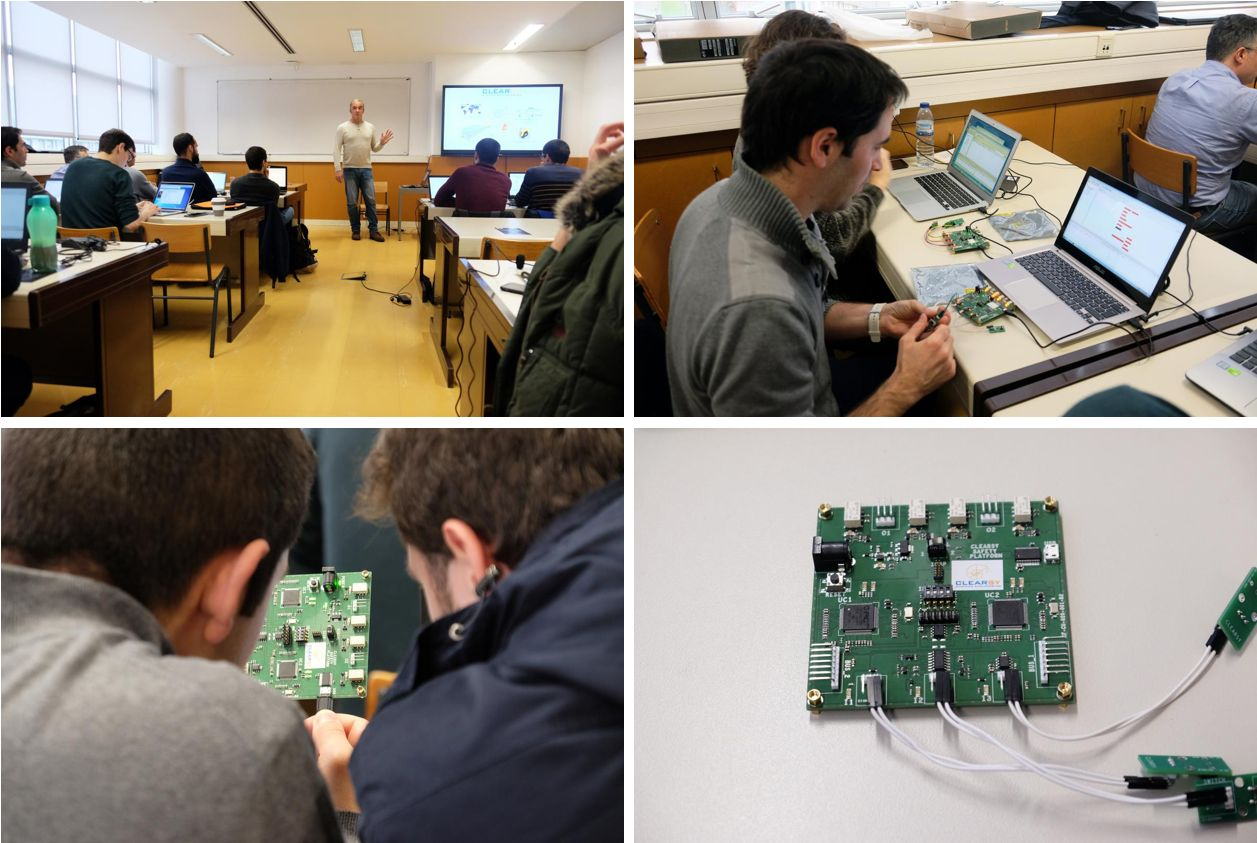
\includegraphics[scale=0.3]{Pictures/FOREWORD-TALK.jpg}
\caption{A busy hands-on session at the University of Minho in Braga, Portugal}
\end{figure}


Particular thanks are due to the team in charge of its development over the past years: Adrien Somoza, Bruno Lavaud, David Deharbe, Denis Sabatier, Eliott Trotebas, Emine Aktepe, Etienne Prun, Florent Patin, Guillaume Pressouyre, Hector Ruiz Barradas, José Tarsitano, Lilian Burdy, Loïc Claudet, Ludovic Delfau, Manfred Winkler, Mathieu Comptier, Maxime Renaud, Patrick Sauvage, Sébastien Agostini, Sylvain Breux, Thierry Lecomte, Thomas Gonthier, Vivien Galuchot.\\

%
\hspace*{\fill} Aix en Provence, France, July 2019


%---------------------------------------------------------------------
%	INTRODUCTION
%---------------------------------------------------------------------
\chapterimage{back2.jpg} % Chapter heading image
\chapter{Introduction}

Developing safety critical applications often requires rare human resources to complete successfully, while off-the-shelf block solutions appear difficult to adapt especially during short-term projects. The CLEARSY Safety Platform fulfils a need for a technical solution to overcome the difficulties of developing SIL3/SIL4 system with its technology based on a double-processor and a formal method with proof to ensure safety at the highest level\cite{lecomte2016double}. The formal method, namely the B method\cite{Abrial.1996}, has been heavily used in the railway industry for decades\cite{DBLP:conf/fmics/Lecomte09}\cite{DBLP:conf/fm/Lecomte08}\cite{DBLP:journals/entcs/Benveniste11}. Using its IDE, Atelier B, to program the CLEARSY Safety Platform ensures a higher level of confidence in the generated software.\\

\begin{figure}[h]
\centering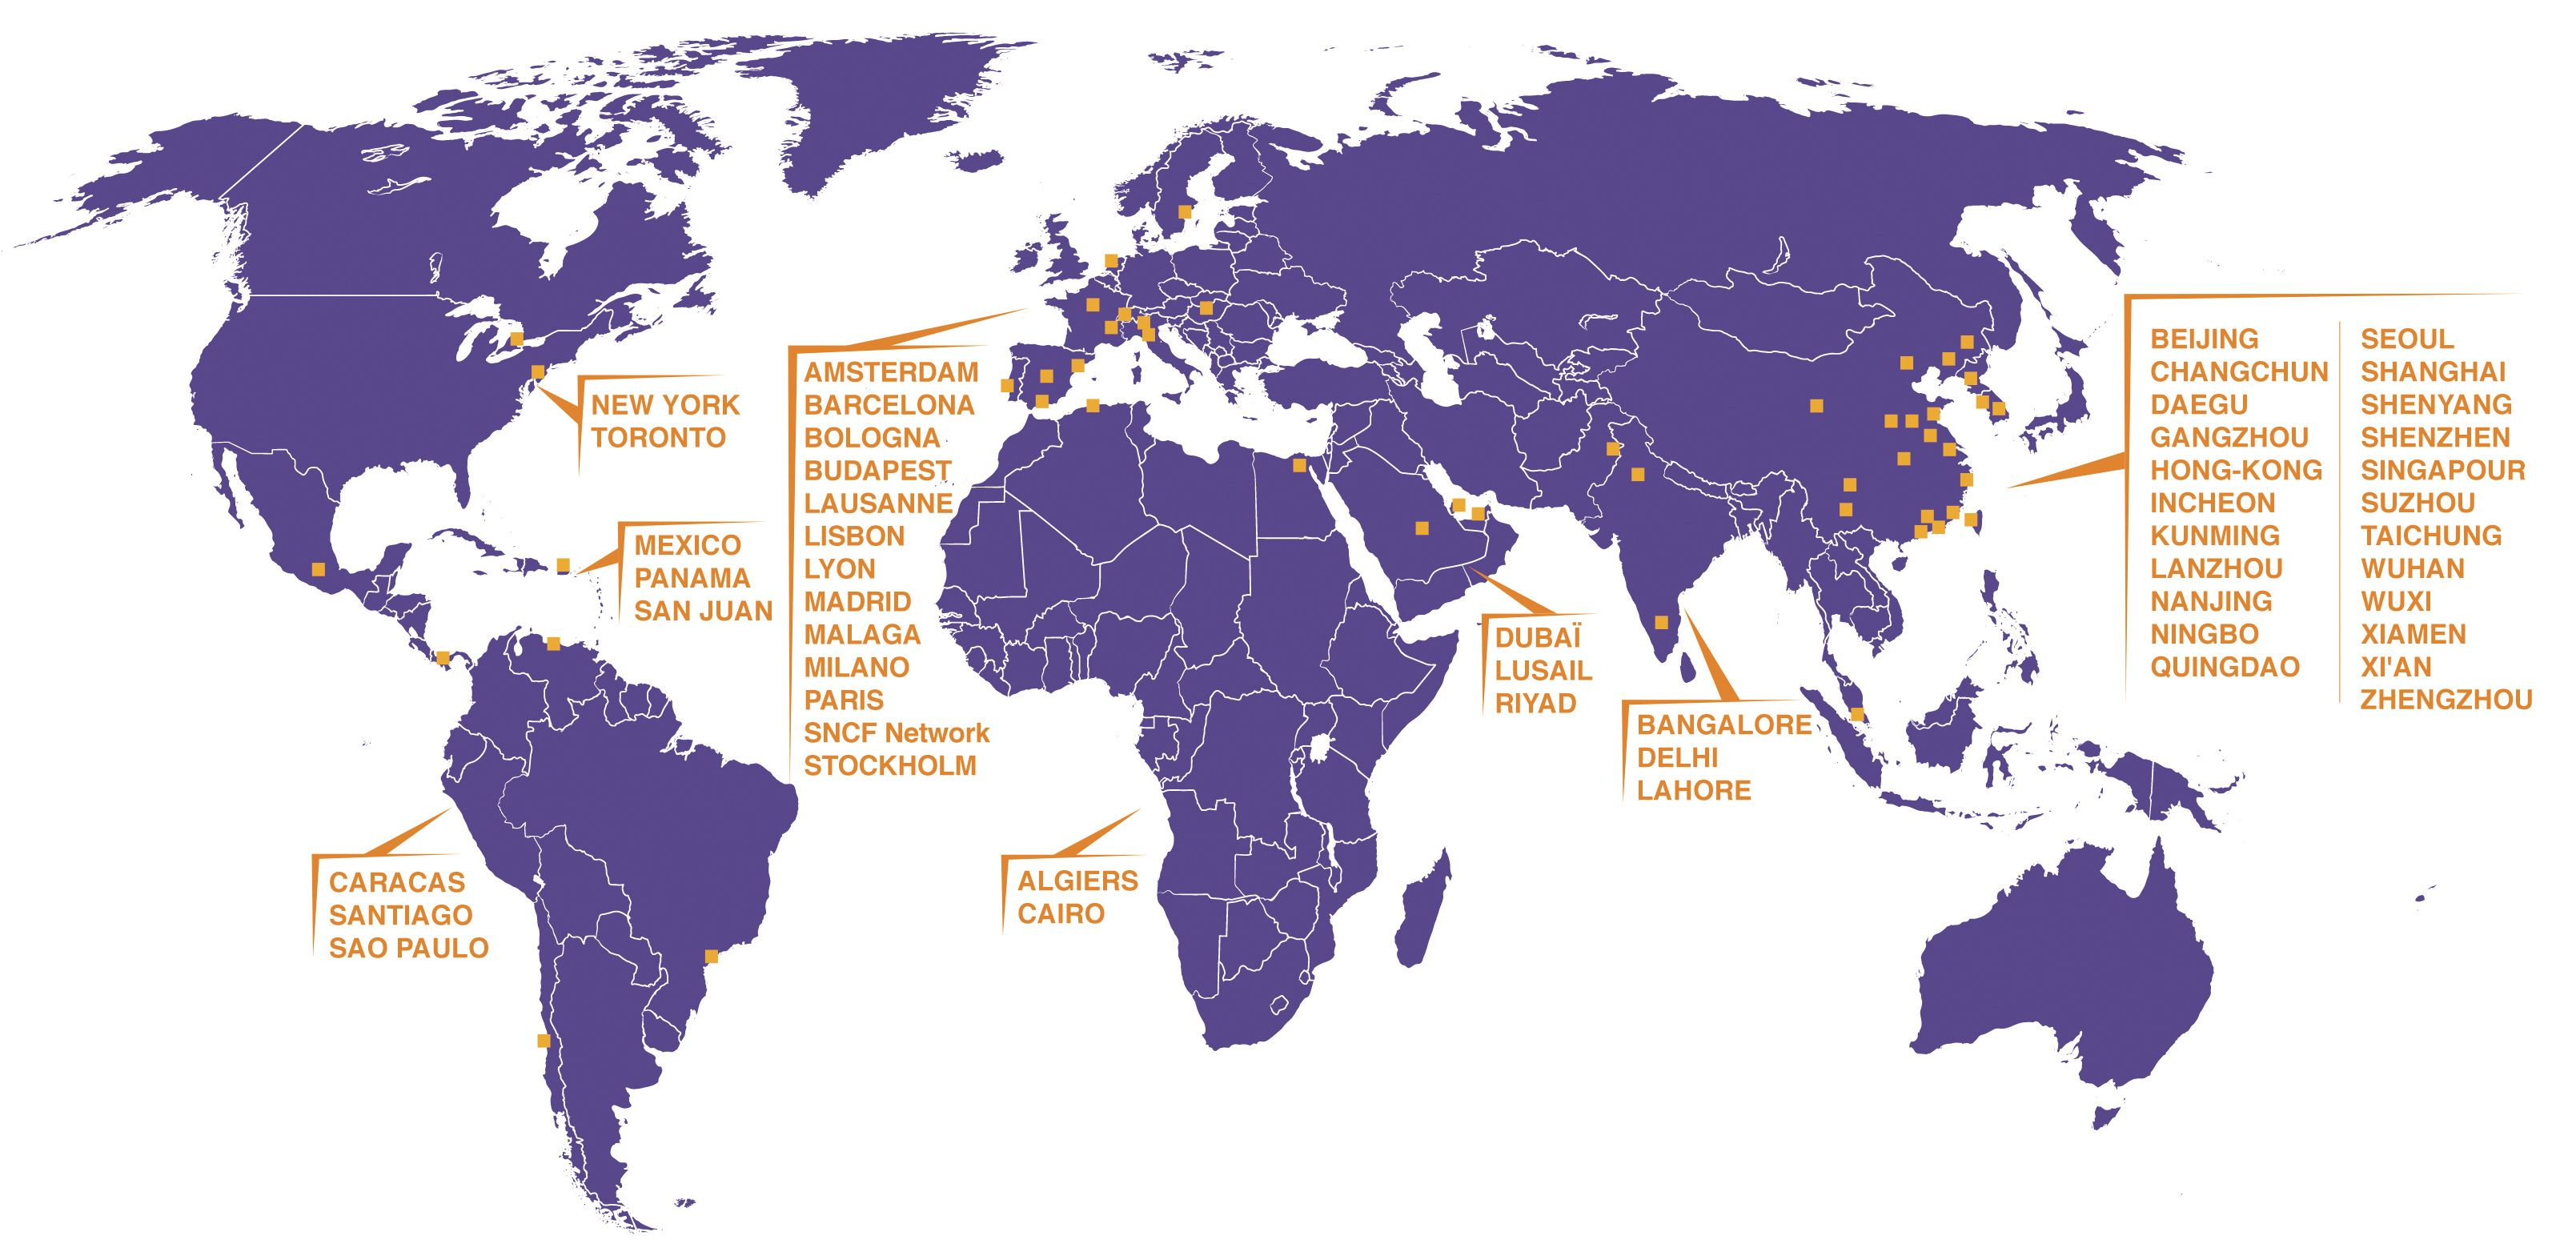
\includegraphics[scale=0.5]{Pictures/INTRO-AtelierB.jpg}
\caption{Metros and trains equipped with B SIL4 software}
\end{figure}

The CLEARSY Safety Platform is both a software and a hardware platform aimed at designing and executing safety critical applications. Such applications implement a command-control function F (Fig. \ref{intro:F}) which cyclically reads inputs, performs computation, and sets outputs. If the platform integrity is not ensured, the execution of F is stopped while the outputs are deactivated (the safe state of the system should coincide with powerless outputs). 

\begin{figure}[h]
\centering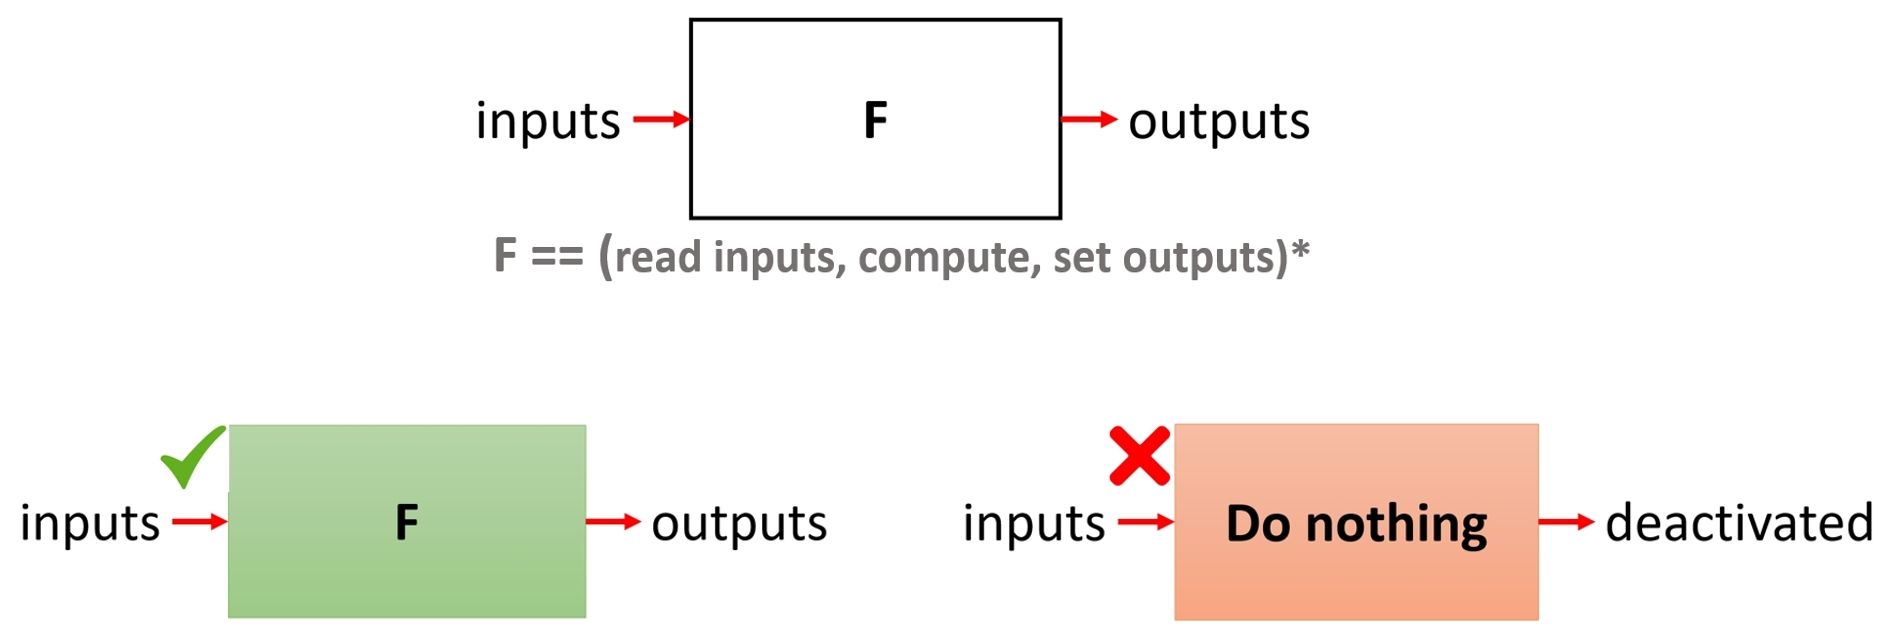
\includegraphics[scale=0.2]{Pictures/Fnew.jpg}
\caption{Execute the right F and execute the F right}
\label{intro:F}
\end{figure}

One formal modelling language is used to program the board. Programs are developed using the dedicated IDE or could be the by-product of some translation from a Domain Specific Language to B. The IDE takes care of the verification of the software (type check, proof, compilation) and then ensures its upload to the hardware platform. The program is guaranteed to execute until a misbehaviour is detected, leading to a safe restricted mode where board outputs are deactivated.\\

The CLEARSY Safety Platform eases the development of safety critical applications as:
\begin{itemize}
    \item it covers the whole development cycle,
    \item the safety principles are built-in and are out of reach of the developer, who cannot alter them,
    \item it is based on a formal language (B) and related proof tools,
    \item the mathematical proof replaces unit and integration testing.\\
\end{itemize}

\begin{figure}[h]
\centering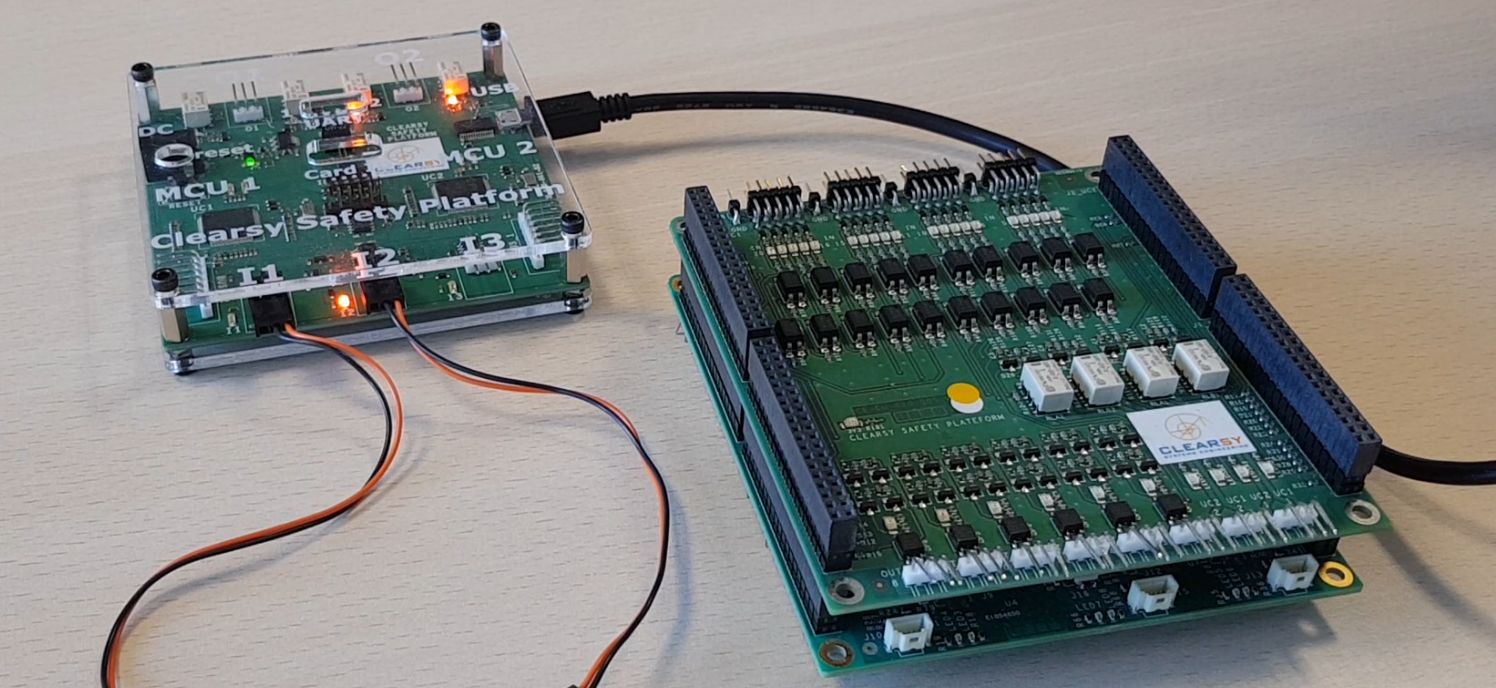
\includegraphics[scale=0.25]{Pictures/INTRO-SK0+SK1.jpg}
\caption{Starter kits SK$_0$ (left) and SK$_1$ (right)}
\end{figure}

%
The CLEARSY Safety Platform eases the certification of safety critical applications as:
\begin{itemize}
    \item the safety cannot be altered by the developer,
    \item it will come with a certification kit.\\
\end{itemize}

The building blocks of the CLEARSY Safety Platform, already certified in international projects during the years 2017 and 2018 by several certification bodies, have been used to develop a generic version of this technology that could fit a broader range of applications. 


The first starter kit, SK$_0$, allows to experiment with the whole development chain, including the IDE, using the B-Method and an electronic board hosting the safe execution platform relying on two PIC32 microcontrollers, providing 3 digital inputs and 2 digital outputs.\\

The second starter kit, SK$_1$, is functionally identical to SK$_0$. It provides 20 digital inputs and 8 digital outputs. The core automaton, with its two PIC32 microcontrollers, is hosted on a motherboard while the inputs/outputs are located on a daughterboard.



%=======================================================================
%	PART I: DESCRIPTION
%=======================================================================
\part{Description}

%---------------------------------------------------------------------
%	Chapter Architecture and Safety Principles
%---------------------------------------------------------------------
\chapterimage{back2.jpg} % Chapter heading image
\chapter{Architecture and Safety Principles}

\section{Introduction to safety}
Safety critical systems are systems where life is at risk. One \textit{mistake} could lead to injury or death (of passengers aboard trains, planes, or cars for example).\\

\noindent One question for a developer is: 
\begin{center}
"would you dare to execute your program if someone would die in case of a crash / core dump / fatal error / etc. especially someone you know like a friend or a member of your family?"    
\end{center}

\begin{figure}[h]
\centering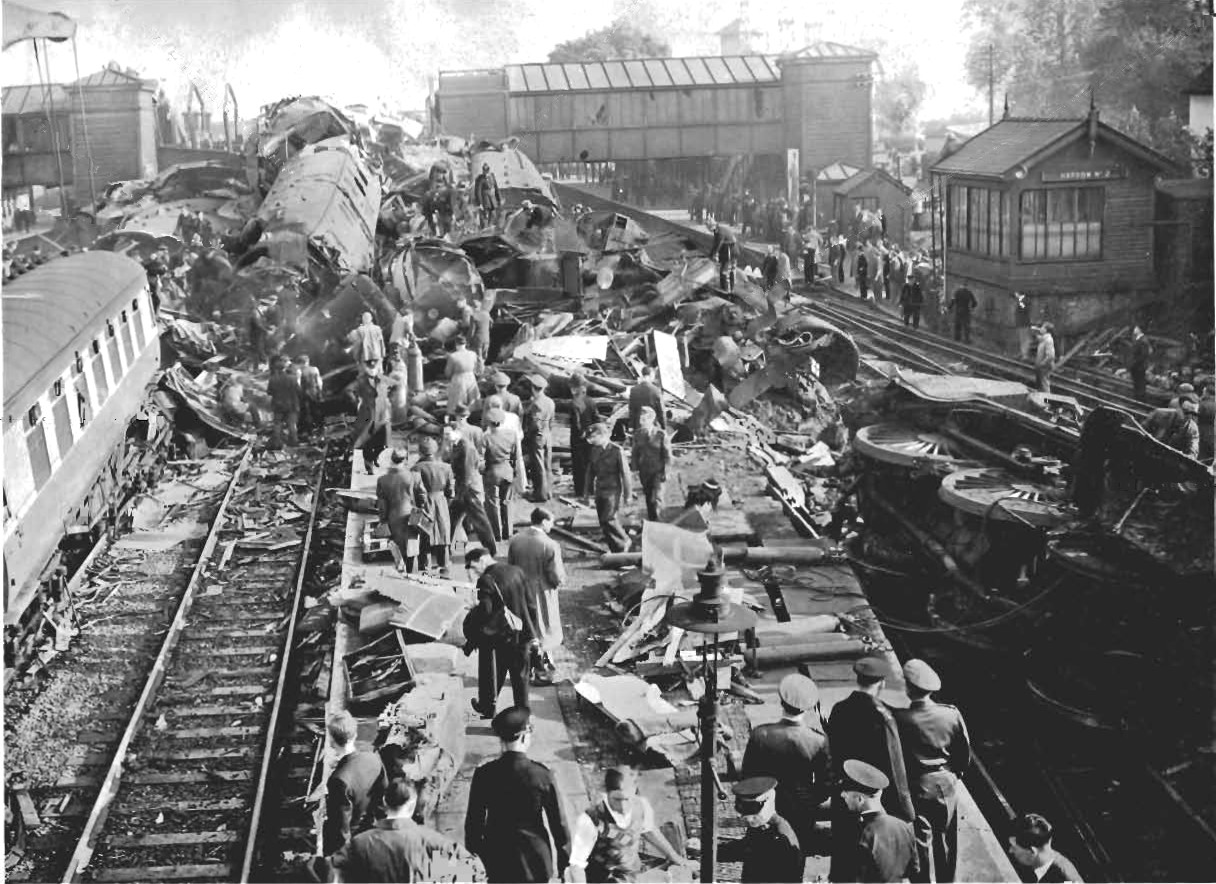
\includegraphics[scale=0.2]{Pictures/chapterSafetyPrinciples/SAFETY-crash.jpg}
\caption{Double collision which occurred on 8th October 1952 at Harrow and Wealdstone Station}
\end{figure}

When you develop a safety system, you are not left alone. Depending on your application domain, you have standards that provide you guidance based on the safety level you are looking for. Note that these standards do not provide a definitive recipe to produce safety systems, but more a collection of state-of-the-art recommendations related to the software, hardware, and development process \footnote{and also maintenance}.

\begin{figure}[h]
\centering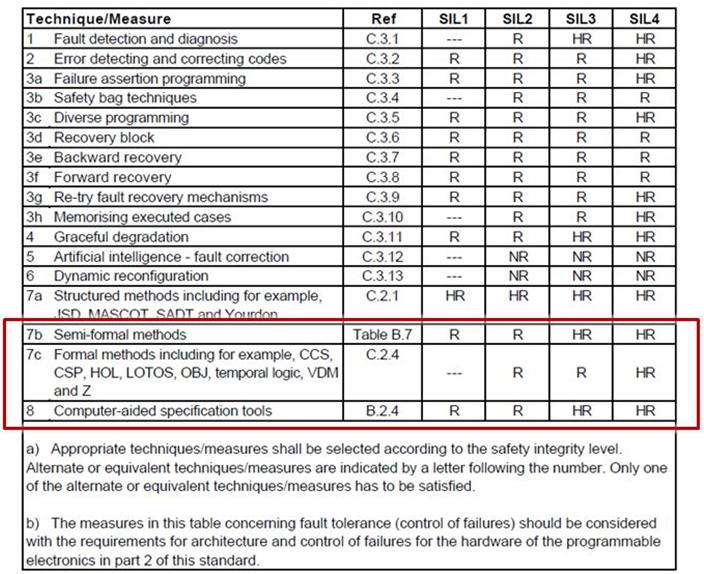
\includegraphics[scale=0.5]{Pictures/chapterSafetyPrinciples/SAFETY-61508A-2.png}
\caption{Table from IEC 61508 standard showing design recommendations for SIL1 to SIL4 software (R: recommended, HR: highly recommended, NR: not recommended. Note that nothing here, including formal methods, is mandatory}
\end{figure}

Before connecting your system to the real world and switching it on, you need to complete a safety case, that is a demonstration the feared event(s)\footnote{in the railway sector, it is mainly train collision} will not happen more frequently than expected. For SIL3, it is one failure every 100 years, and for SIL4, one failure every 10,000 years. \\ 

For the safety case, you need to consider the whole picture: the hardware (computers, sensors, actuators, etc.), the software, and the environment at large. The main question is: 
\begin{center}
    "what could happen in case that something fails?"
\end{center}
We are far from the concept: "it compiles, hence it works". The safety case always depends on a number of hypotheses that restrict the scope. The idea is not to protect against everything but only to consider a set of "reasonable" situations. As an example, for train collision, we do not consider a plane that could crash on the tracks.\\

\noindent The "failures" considered are diverse and represent a large spectrum of situations: 
\begin{itemize}
    \item specification error: we specified the wrong system or software.
    \item development error: the specification is correct but the implementation does not comply with its specification. It could be a functional mistake: the algorithm is doing something different than what is expected. It could be non-functional: the operation is performed slower than expected.
    \item programming error: numbers are divided by 0, arithmetic computation produces overflow, or tables are accessed outside of their range.
    \item compilation error: binary code produced does not comply with source code \footnote{Who is reading the binary code these days?}
    \item wrong execution: the memory is corrupted (wrong data, wrong instruction, corrupted program counter), the hardware is failing (wrong instruction execution, incorrect storage/access)
    \item failing hardware: sensors are providing incorrect values, actuators cannot be commanded properly.
\end{itemize}

For a SIL4 system, the target reliability is between $10^{-7}$/h to $10^{-9}$/h. Given that a processor reliability is estimated between $10^{-4}$/h to $10^{-6}$/h, a single processor is not sufficient for a SIL3 or SIL4 system. That is why two processors (or more) are used in parallel (traditionally with a voter - the two processors have to come to the same decision to initiate a potentially risky action \footnote{for example, opening platform screen doors on a metro platform with the risk that waiting passengers could fall on the tracks if no train is present}. In addition, the two processors are equipped with protecting mechanisms that would allow the system to continue its mission in case of perturbation / failure.  



\begin{figure}[h]
\centering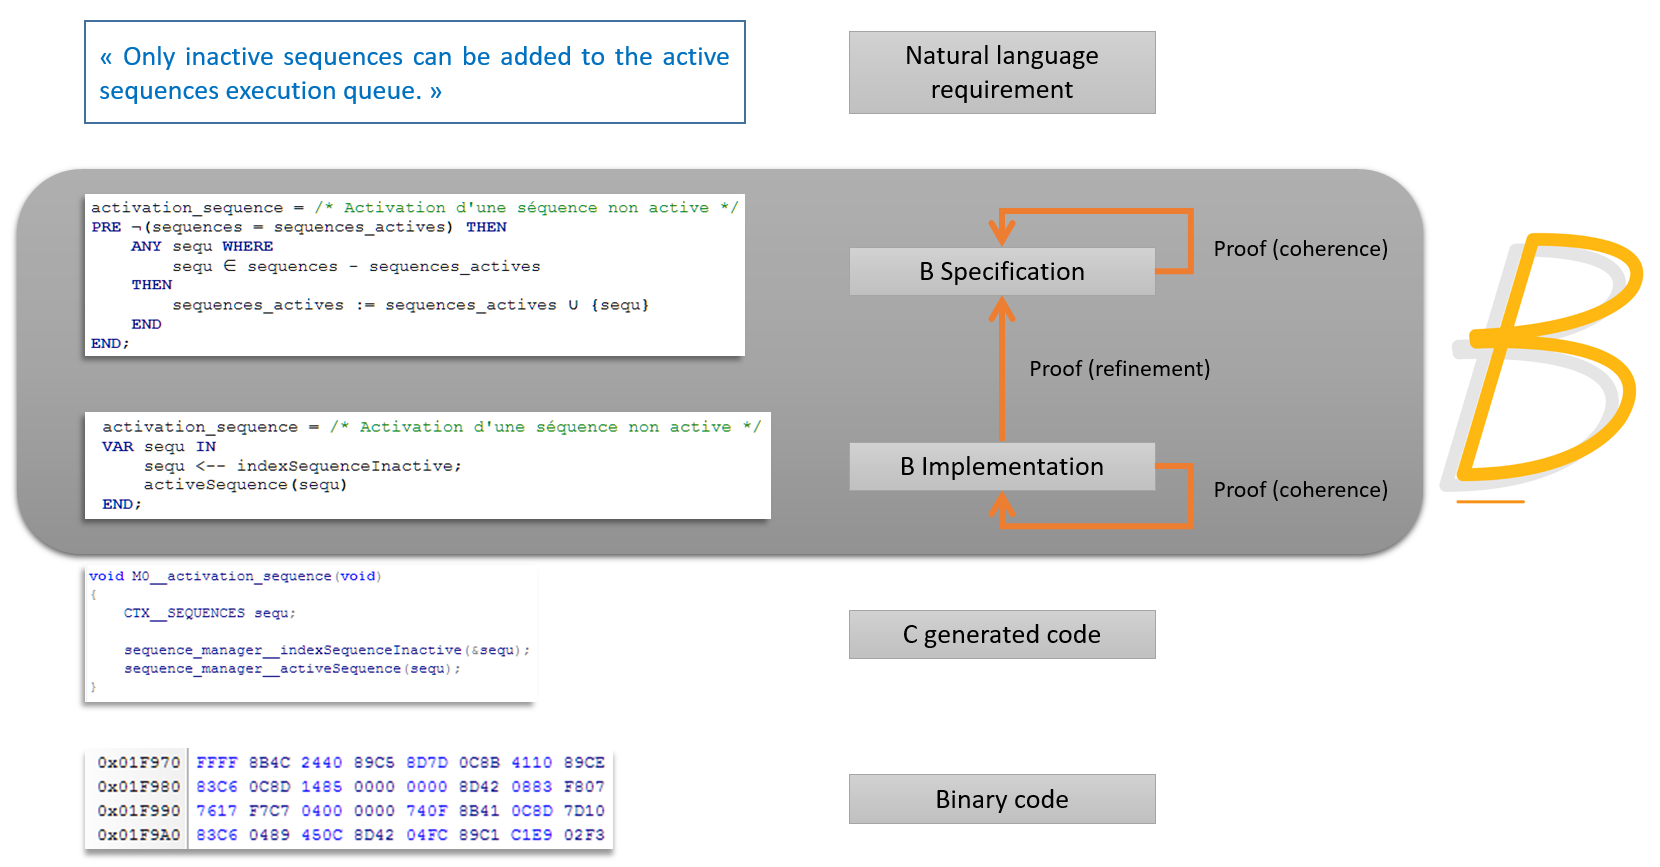
\includegraphics[scale=0.3]{Pictures/chapterSafetyPrinciples/SAFETY-Bcycle.png}
\caption{Path from requirements to binary code with B}
\label{safety:B}
\end{figure}

The contribution of B to the safety case is explained in figure \ref{safety:B}. In this figure, we see the different stages from requirements to binary code (from top to bottom). The B method covers the software specification and implementation stages (the grey box) where the specification and implementation models are proved (we will see later on what it means). However the inputs and outputs of this grey box are error prone:
\begin{itemize}
    \item the specification model could be different from the natural language requirements. Usually human based cross verification is required - every requirement should be in the model, every modelling element should be issued from the natural language requirements. Validation testing also helps to find mistakes at this stage.
    \item the code generated could be different from the implementation model: the code generator may alter the semantics of the implementation model due to incorrect code generator specification or bugs.
    \item the binary code could be different form the source code: the compiler may alter the semantics of the source code, due to improper optimisation options or bugs.
    \item the processor executing the binary code could exhibit a misbehaviour due to either internal reasons (design or production flaw) and/or external reasons (high energy particles, electromagnetic waves, etc.).\\
\end{itemize}

Usually the last three bullets are taken into account with diversity, given that the program is executed on two (or more) processors: two different code generators are used to produce two different source codes from the same formal model. It is very unlikely that two tools developed with different technologies (programming language, libraries, compiler) and by independent teams are going to exhibit the same unsafe behaviour under the same conditions. One code generator could for example use a big endian memory model while the other uses a little endian one. Another option is to add void instructions \footnote{One code could be xx := yy + zz while the other is xx := yy + zz + 1 - 1 } in one source code only that do not change the final behaviour but produce a different binary code. That way a processor perturbation would not affect the two programs the same way because different parts of each program are being executed.\\

We can clearly see that in the case of safety systems, the B method is only one part of the story and other means have to be set up in order to reach safety related objectives. These means require rare human resources to complete successfully because of the deep level of understanding of both hardware and software parts to consider. \\

\begin{figure}[h]
\centering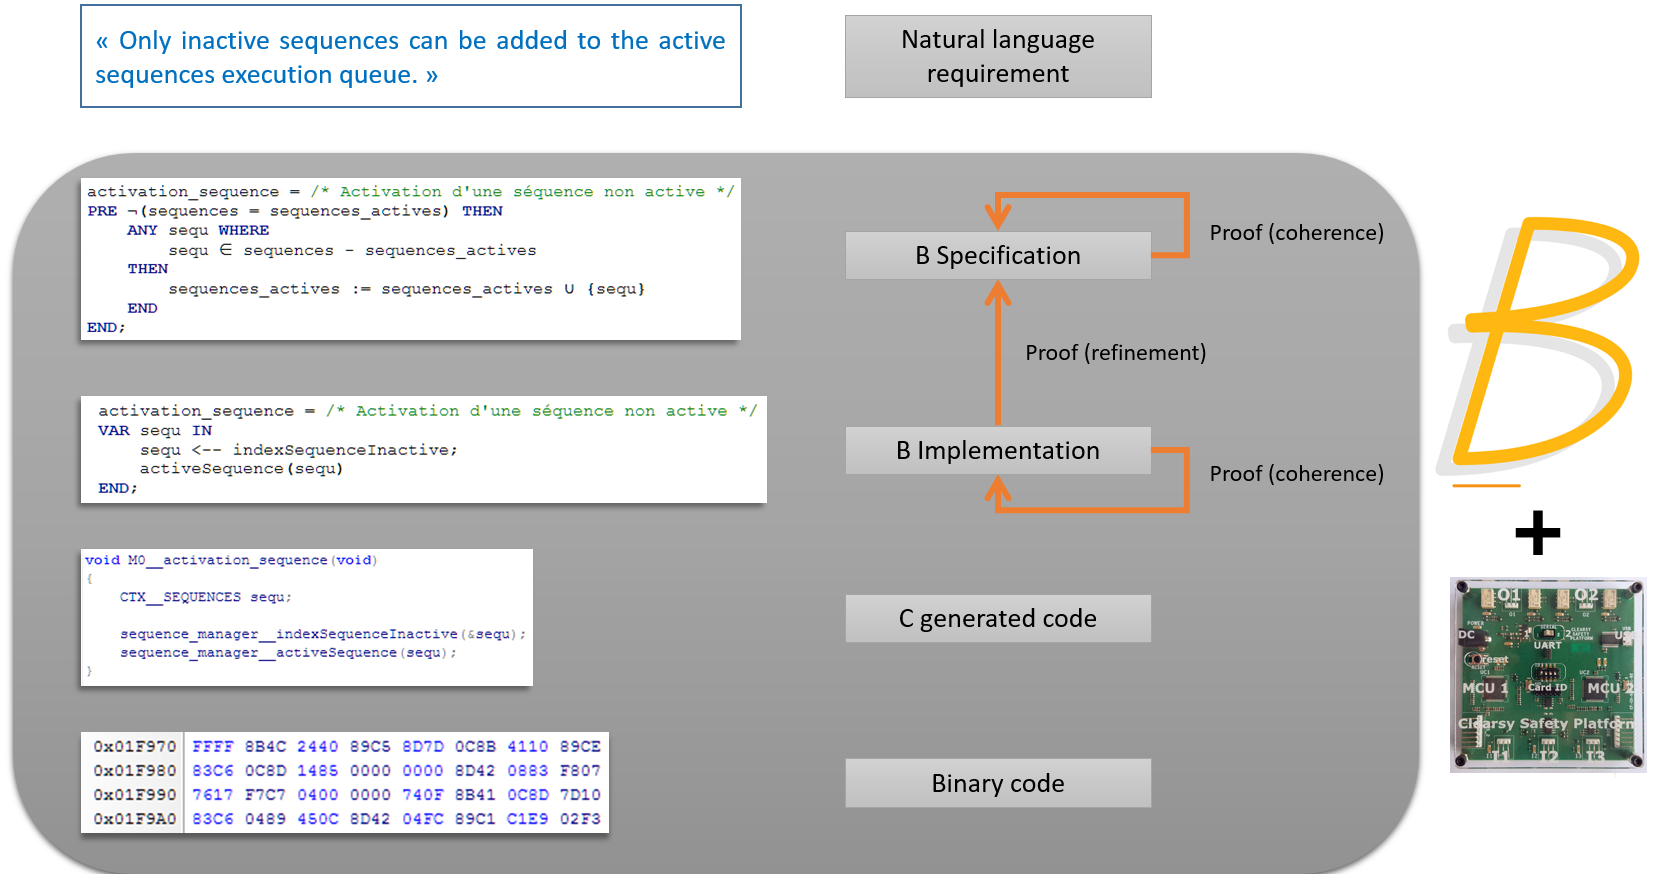
\includegraphics[scale=0.3]{Pictures/chapterSafetyPrinciples/SAFETY-BCSSPcycle.png}
\caption{Path from requirements to binary code with B with the CLEARSY Safety Platform}
\label{safety:CSSP}
\end{figure}

With the CLEARSY Safety Platform, the very technical aspects related to safety are taken into account by the platform (see chapter \ref{safety:safety-principles}), leaving the developer to focus only on the development of the function to perform. In the figure \ref{safety:CSSP}, the combination of B and CSSP covers all the steps from software specification to binary code. The developer is only required to be able to specify and program in B (with DSL if a translator from DSL to B is available), thus less expert profiles could be used for the development. The only remaining activity to perform (apart from validation testing, always mandatory) is the traceability/coverage between natural language requirement and formal modelling. Hence the CLEARSY Safety Platform, with its technology based on a double processor and a formal method with proof to ensure safety at the highest level, fulfils the need for a technical solution to overcome the difficulties of developing SIL3/SIL4 systems.

\section{Architecture}

The CLEARSY Safety Platform  is made of two parts: an IDE to develop the software and an electronic board to execute this software. The full process is described in figure \ref{arch:principes}.

\begin{figure}[h]
\centering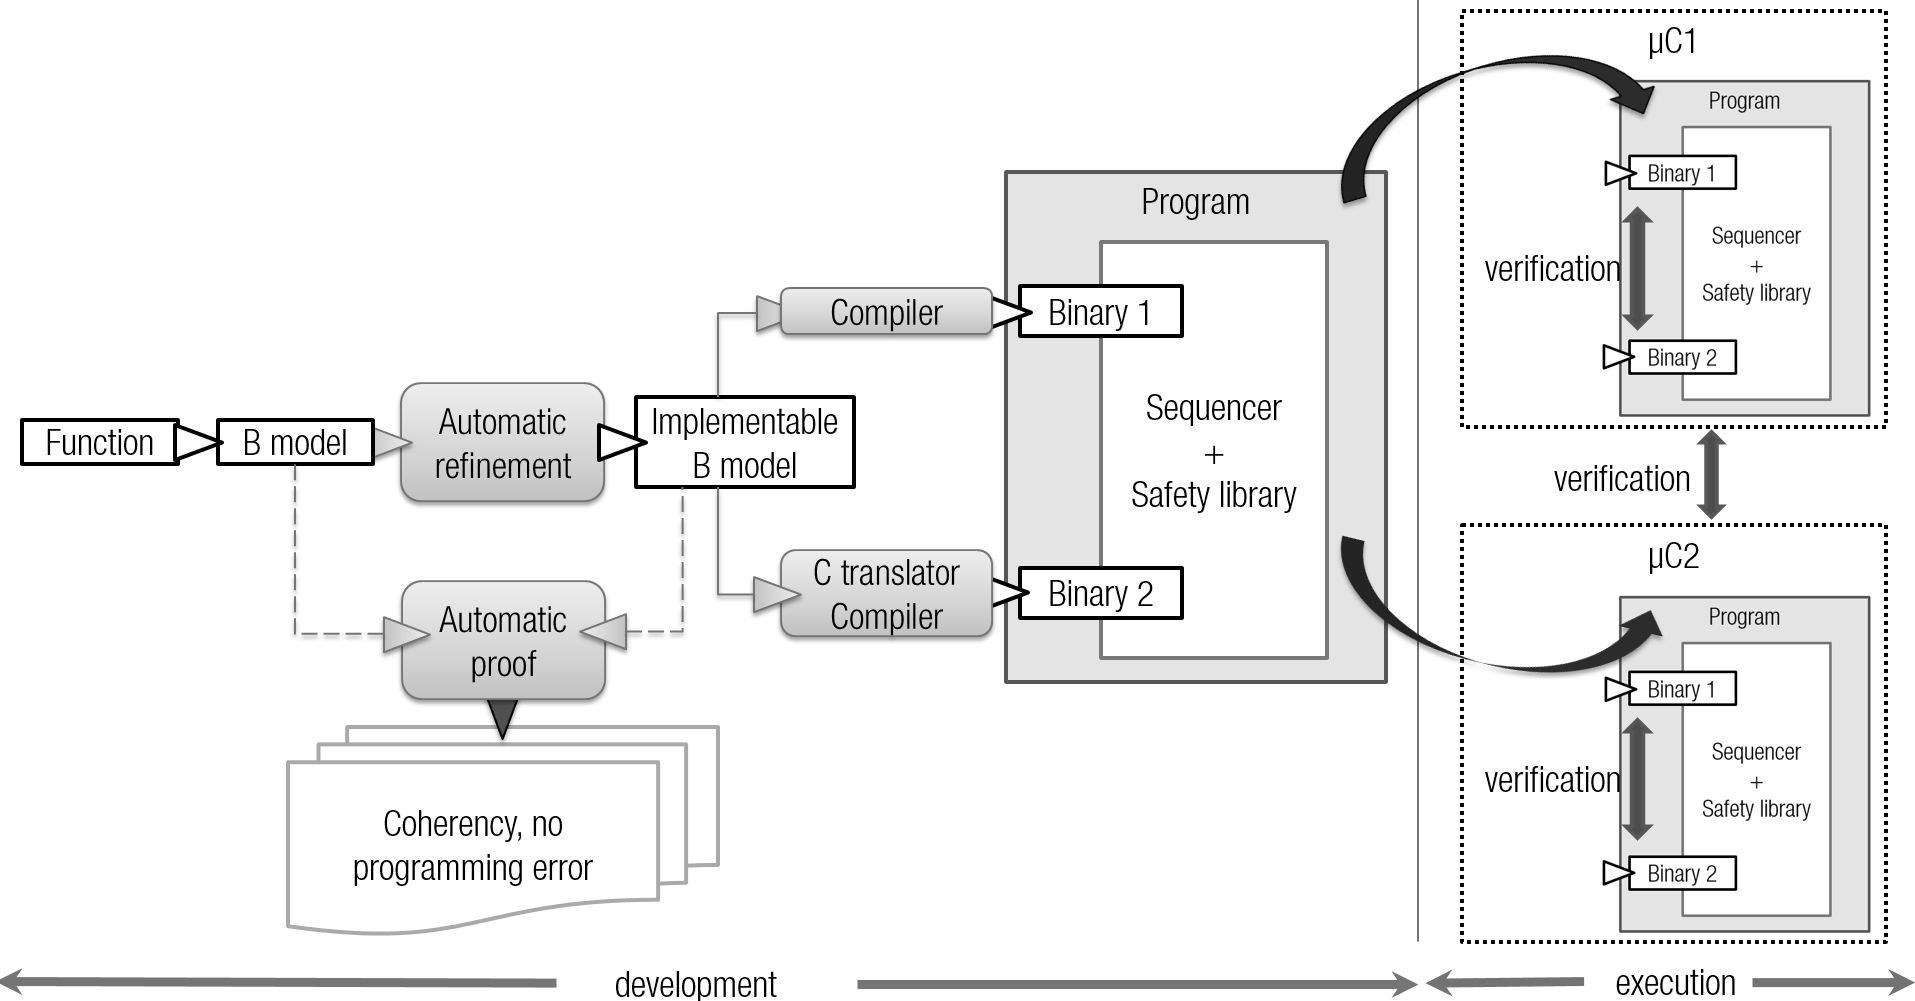
\includegraphics[scale=0.24]{Pictures/chapterSafetyPrinciples/ARCH-LCHIP-principe.jpg}
\caption{Full path from function description to safe execution with the CLEARSY Safety Platform. Round boxes are tools, rectangular boxes are files.}
\label{arch:principes}
\end{figure}

It starts with the function specification (natural language) to develop. The developer has to provide a B model of it (specification and implementation) using the schema:
\begin{itemize}
    \item the function to program is a loop, where the following steps are performed repeatedly in sequence:
\begin{itemize}
    \item the inputs are read \footnote{Inputs are similar for $\mu C_1$ and $\mu C_2$, unless the inputs are captured at different times in which case the different values would cause the platform to enter panic mode.}
    \item some computation is performed
    \item the outputs are set
\end{itemize}
\item The steps related to inputs and outputs are fixed and cannot be modified. 
\item Only the computation may be modified to obtain the desired behaviour.\\
\end{itemize}


The implementation is usually handwritten but could also be generated automatically with the B Automatic Refinement Tool \footnote{However automatic refinement requires a higher level of experience of B and is not covered in this book.}. The B models are proved (mostly automatically as the level of abstraction of typical command \& control applications is low) to be coherent and to contain no programming error.
From the implementable model, two binaries are generated:
\begin{itemize}
    \item binary$_1$, obtained via a dedicated compiler (developed by CLEARSY) transforming a B model into HEX \footnote{"Intel HEX is a file format that conveys binary information in ASCII text form. It is commonly used for programming microcontrollers, EPROMs, and other types of programmable logic devices." (Wikipedia)} file,
    \item binary$_2$, produced with the Atelier B C code generator then compiled with the GCC compiler into another HEX file.
\end{itemize} 
Each binary represents the same function but is supposed to be made of different sequences of instructions because of the diversity of the tool chains. 
Then the two binaries binary$_1$ and binary$_2$ are linked with:
\begin{itemize}
    \item a sequencer, in charge of reading inputs, executing binary$_1$ then binary$_2$, and setting the outputs
    \item a safety library, in charge of performing safety verification (more details in chapter \ref{safety:safety-principles}). In case of failing verification, the board enters panic mode, meaning the outputs are deactivated \footnote{No power is provided to the Normally Open (NO) outputs, so the output electric circuits are open.}, the board status LED start flashing, and the board enters an infinite loop doing nothing. A hard reset (power off or reset button) is the only possibility to interrupt this panic mode.
\end{itemize}
The final program is thus made of binary$_1$, binary$_2$, the sequencer and the safety library. The memory mappings of binary$_1$ and binary$_2$ are separate. 

This program is then uploaded on the two micro-controllers $\mu C_1$ and $\mu C_2$. The bootloader, on the electronic board, checks the integrity of the program (CRC, separate memory spaces). Then both micro-controllers start to execute the program. During its execution, the following are performed:
\begin{itemize}
    \item internal verification:
\begin{itemize}
    \item every cycle, binary$_1$ and binary$_2$ memory spaces (variables) are compared
    \item regularly, binary$_1$ and binary$_2$ memory spaces (program) are compared \footnote{This verification is performed "in the background" over thousands/millions of cycles, to keep a reasonable cycle time.}
    \item regularly, the identity between memory output states and physical output states is checked to detect if the board is unable to command the outputs.
\end{itemize} 
\item external verification:
\begin{itemize}
    \item regularly (every 50ms at the latest), memory spaces (variables) are compared between $\mu C_1$ and $\mu C_2$. 
\end{itemize} 
\end{itemize} 
If any of these verifications fail, the board enters the panic mode.

The whole process is fully supported by adequate tools. In the figure \ref{arch:process}, the tools and text/binary files generated are made explicit for both the application (path used every time an application is developed) and the safety belt (developed once for all by the IDE development team \footnote{Note that from the abstract formal model, one part of the software is developed in B with concrete formal model, while the other part is developed manually. It happens when using B provides no added-value (for example low-level IO). A component modelled in B and implemented manually is called a basic machine.}. The tools are issued from Atelier B, except:
\begin{itemize}
    \item the B to HEX compiler, initially developed to control platform screen doors for metro lines in Brazil. This tool proceeds in two steps: a translation from B to ASM MIPS, then from ASM MIPS to HEX \footnote{In order to ease debugging as ASM MIPS to HEX is a straightforward line-to-line translation.}.
    \item the C to HEX GCC compiler.
    \item the linker combining the 2 hex files with the safety sequencer and libraries.
    \item the bootloade.r\\
\end{itemize}



We can clearly see that the CLEARSY Safety Platform is a generic PLC \footnote{"A Programmable Logic Controller is an industrial digital computer which has been ruggedized and adapted for the control of manufacturing processes, such as assembly lines, or robotic devices, or any activity that requires high reliability control and ease of programming and process fault diagnosis." (wikipedia)} able to perform command and control over inputs and outputs. The overall architecture is similar between all instances of the CLEARSY Safety Platform. The differences are due to the physical interface:
\begin{itemize}
    \item 5 IOs for SK$_0$, 28 for SK$_1$.
    \item digital (Boolean) IOs for SK$_0$ and SK$_1$, analog IOs in the future.
    \item network connection (messaging) through a maintenance processor, in the future.
\end{itemize}

\begin{remark}
From a safety point of view, the current architecture is valid for any kind of mono-core processor. The decision of using PIC32 micro-controllers (able to deliver around 50 DMIPS) was made based on our knowledge and experience of this processor. Implementing the CLEARSY Safety Platform on other hardware \footnote{STM32 for example} would "only" require the existing electronic board and software tools to be modified, without impacting much the safety demonstration.
\end{remark} 

\begin{figure}[h]
\centering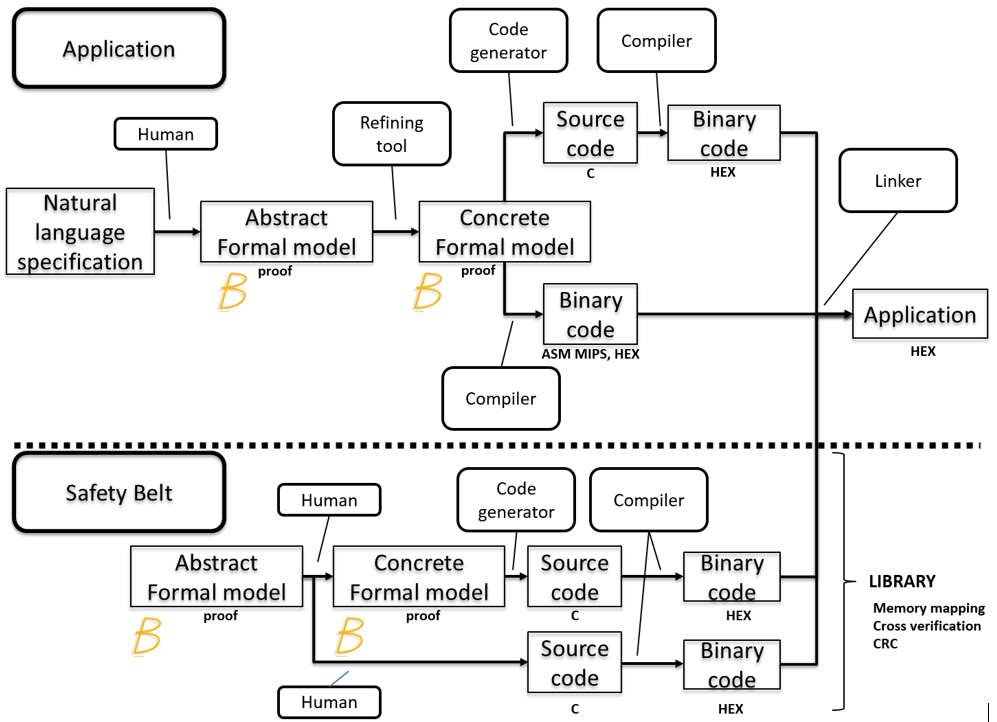
\includegraphics[scale=0.35]{Pictures/chapterSafetyPrinciples/ARCH-LCHIP-process.jpg}
\caption{Tools and files involved in the generation of the software}
\label{arch:process}
\end{figure}



\section{Safety Principles}
\label{safety:safety-principles}

The safety is built on top of few principles:
\begin{itemize}
    \item a B formal model of the function to develop, proved to be coherent, to correctly implement its specification, and to be programming error-free,
    \item four instances of the same function running on two micro-controllers (two per micro-controller with different binaries obtained from diverse tool-chains) and the detection of any divergent behaviour among the four instances,
    \item the deferred cross-verification of the programs on the two $\mu C$,
    \item outputs require both $\mu C_1$ and $\mu C_2$ to be alive and running as one provides energy and the other one the command,
    \item output physical states are regularly verified to comply with the memory states, to check the ability of the board to command its outputs,
    \item input signals are continuous (0 or 5V) and are made dynamic (addition of a frequency signal) in order to prevent the short-circuit current from being considered  as high level (permissive) logic.
\end{itemize}

\begin{table}[ht]
\small
\begin{tabular}{|l|c|l|l|}
\hline
\textbf{Stage} & \textbf{\#} &  \textbf{Failure}                  & \textbf{CSSP verification} \\ \hline
specification  & 1 & Typing error                      & Typechecker tool detects typing error \\ \hline
specification  & 2 & Specified behaviour incompatible  & Unprovable proof obligation indicates   \\
               & & with invariant properties         & specification mistake       \\ \hline           
implementation & 3 & Typing error                      & Typechecker tool detects typing error \\ \hline
implementation &   & Implemented behaviour incompatible  & Unprovable proof obligation indicates   \\
               &   & with invariant properties         & implementation mistake       \\ \hline           
implementation & 4 & Implemented behaviour incompatible  & Unprovable proof obligation indicate   \\
               &   & with specified behaviour          & implementation mistake       \\ \hline 
implementation & 5 & Overflow capable arithmetic operators  & Detected by the B-to-HEX compiler   \\
               &   & used instead of dedicated ones     &       \\ \hline 
implementation & 6 & IF clause with more than one condition  & Detected by the B-to-HEX compiler   \\
               &   & (B0 language restriction)          &       \\ \hline 
implementation & 7 & LOCAL variables not typed before use  & Detected by the B-to-HEX compiler   \\
               &   & (B0 language restriction)          &       \\ \hline                
code generation & 8 & Syntax errors in the C generated code  & Detected by the MICROCHIP compiler   \\  \hline
code generation & 9 & Incorrect naming in the C         & Detected by the linker   \\            
                &   & generated code                    &           \\ \hline  
code generation & 10 & Incorrect memory map             & Memory overlap detected by the   \\  
                &    &                                 &  bootloader   \\ \hline 
\end{tabular}
\caption{Verification performed during development}
\label{safety:verif-dev}
\end{table}     
 However, as explained in the chapter \ref{preface}, the electronic board lacks some vital elements to comply with highest SIL requirements like:
 \begin{itemize}
     \item ensure galvanic isolation between the two half-boards, to prevent that one side of the board wrongly provides energy to the other side's outputs,
     \item activate safety outputs with a sinusoidal signal \footnote{The micro-controller needs to be alive to generate the sinusoidal signal.} instead of a continuous signal, to ignore fault current and activate output.
 \end{itemize}
These missing features are only needed for real-life safety critical systems and do not prevent developers, whether students, researchers or engineers, from using the CLEARSY Safety Platform for education and prototype development. 

The verification performed by the CLEARSY Safety Platform, either during development or execution stages, is summarised in tables \ref{safety:verif-dev} and \ref{safety:verif-exec}.
\begin{table}[ht]
\small
\begin{tabular}{|l|c|l|l|}
\hline
\textbf{Stage} & \textbf{\#} &  \textbf{Failure}                  & \textbf{CSSP verification} \\ \hline                
compilation    & 11 & Wrong binary code generated       & Detected during execution by safety \\
               &    &                                   & library by comparing binary$_1$ and  \\ 
               &    &                                   &  binary$_2$ variables in memory\\ 
               &    &                                   & with CRC on the same $\mu C$ \\ \hline
uploading      & 12 & Incorrect transfer between host   & Detected by bootloader during upload (CRC)\\
               &    & and electronic board              & and during execution over several cycles\\ \hline

execution      & 13 & RAM error (variables)             & Detected by comparing binary$_1$ \\
               &    &                                   & and binary$_2$ variables in memory \\
               &    &                                   & with CRC on the same $\mu C$ \\ \hline
execution      & 14 & RAM error (program)             & Detected by comparing binary$_1$ \\
               &    &                                   & and binary$_2$ program in memory \\
               &    &                                   & with CRC with the other $\mu C$ \\ \hline
execution      & 15 & Failure of one $\mu C$        & Detected by handshake between $\mu C_1$  \\ 
               &    &                               & and $\mu C_2$ at least every 50 ms \\ \hline
execution      & 16 & Outputs not command-able       & Detected by checking physical state  \\ 
               &    &                               & and command issued by the software \\
\hline
\end{tabular}
\caption{Verification performed during execution}
\label{safety:verif-exec}
\end{table}







%---------------------------------------------------------------------
%	Chapter Programming
%---------------------------------------------------------------------
\chapterimage{back2.jpg} % Chapter heading image
\chapter{Programming}

\section{Installation}

The starter kit SK$_0$ is composed of: 
\begin{itemize}
    \item The CLEARSY Safety Platform board
    \item A micro-USB connector to upload the software and to monitor its execution
    \item A power supply
    \item 3 switches connected to the 3 digital inputs I$_1$, I$_2$ and I$_3$
    \item The development environment running on Windows
    \item The user manual (this book)
\end{itemize}

\begin{figure}[ht]
\centering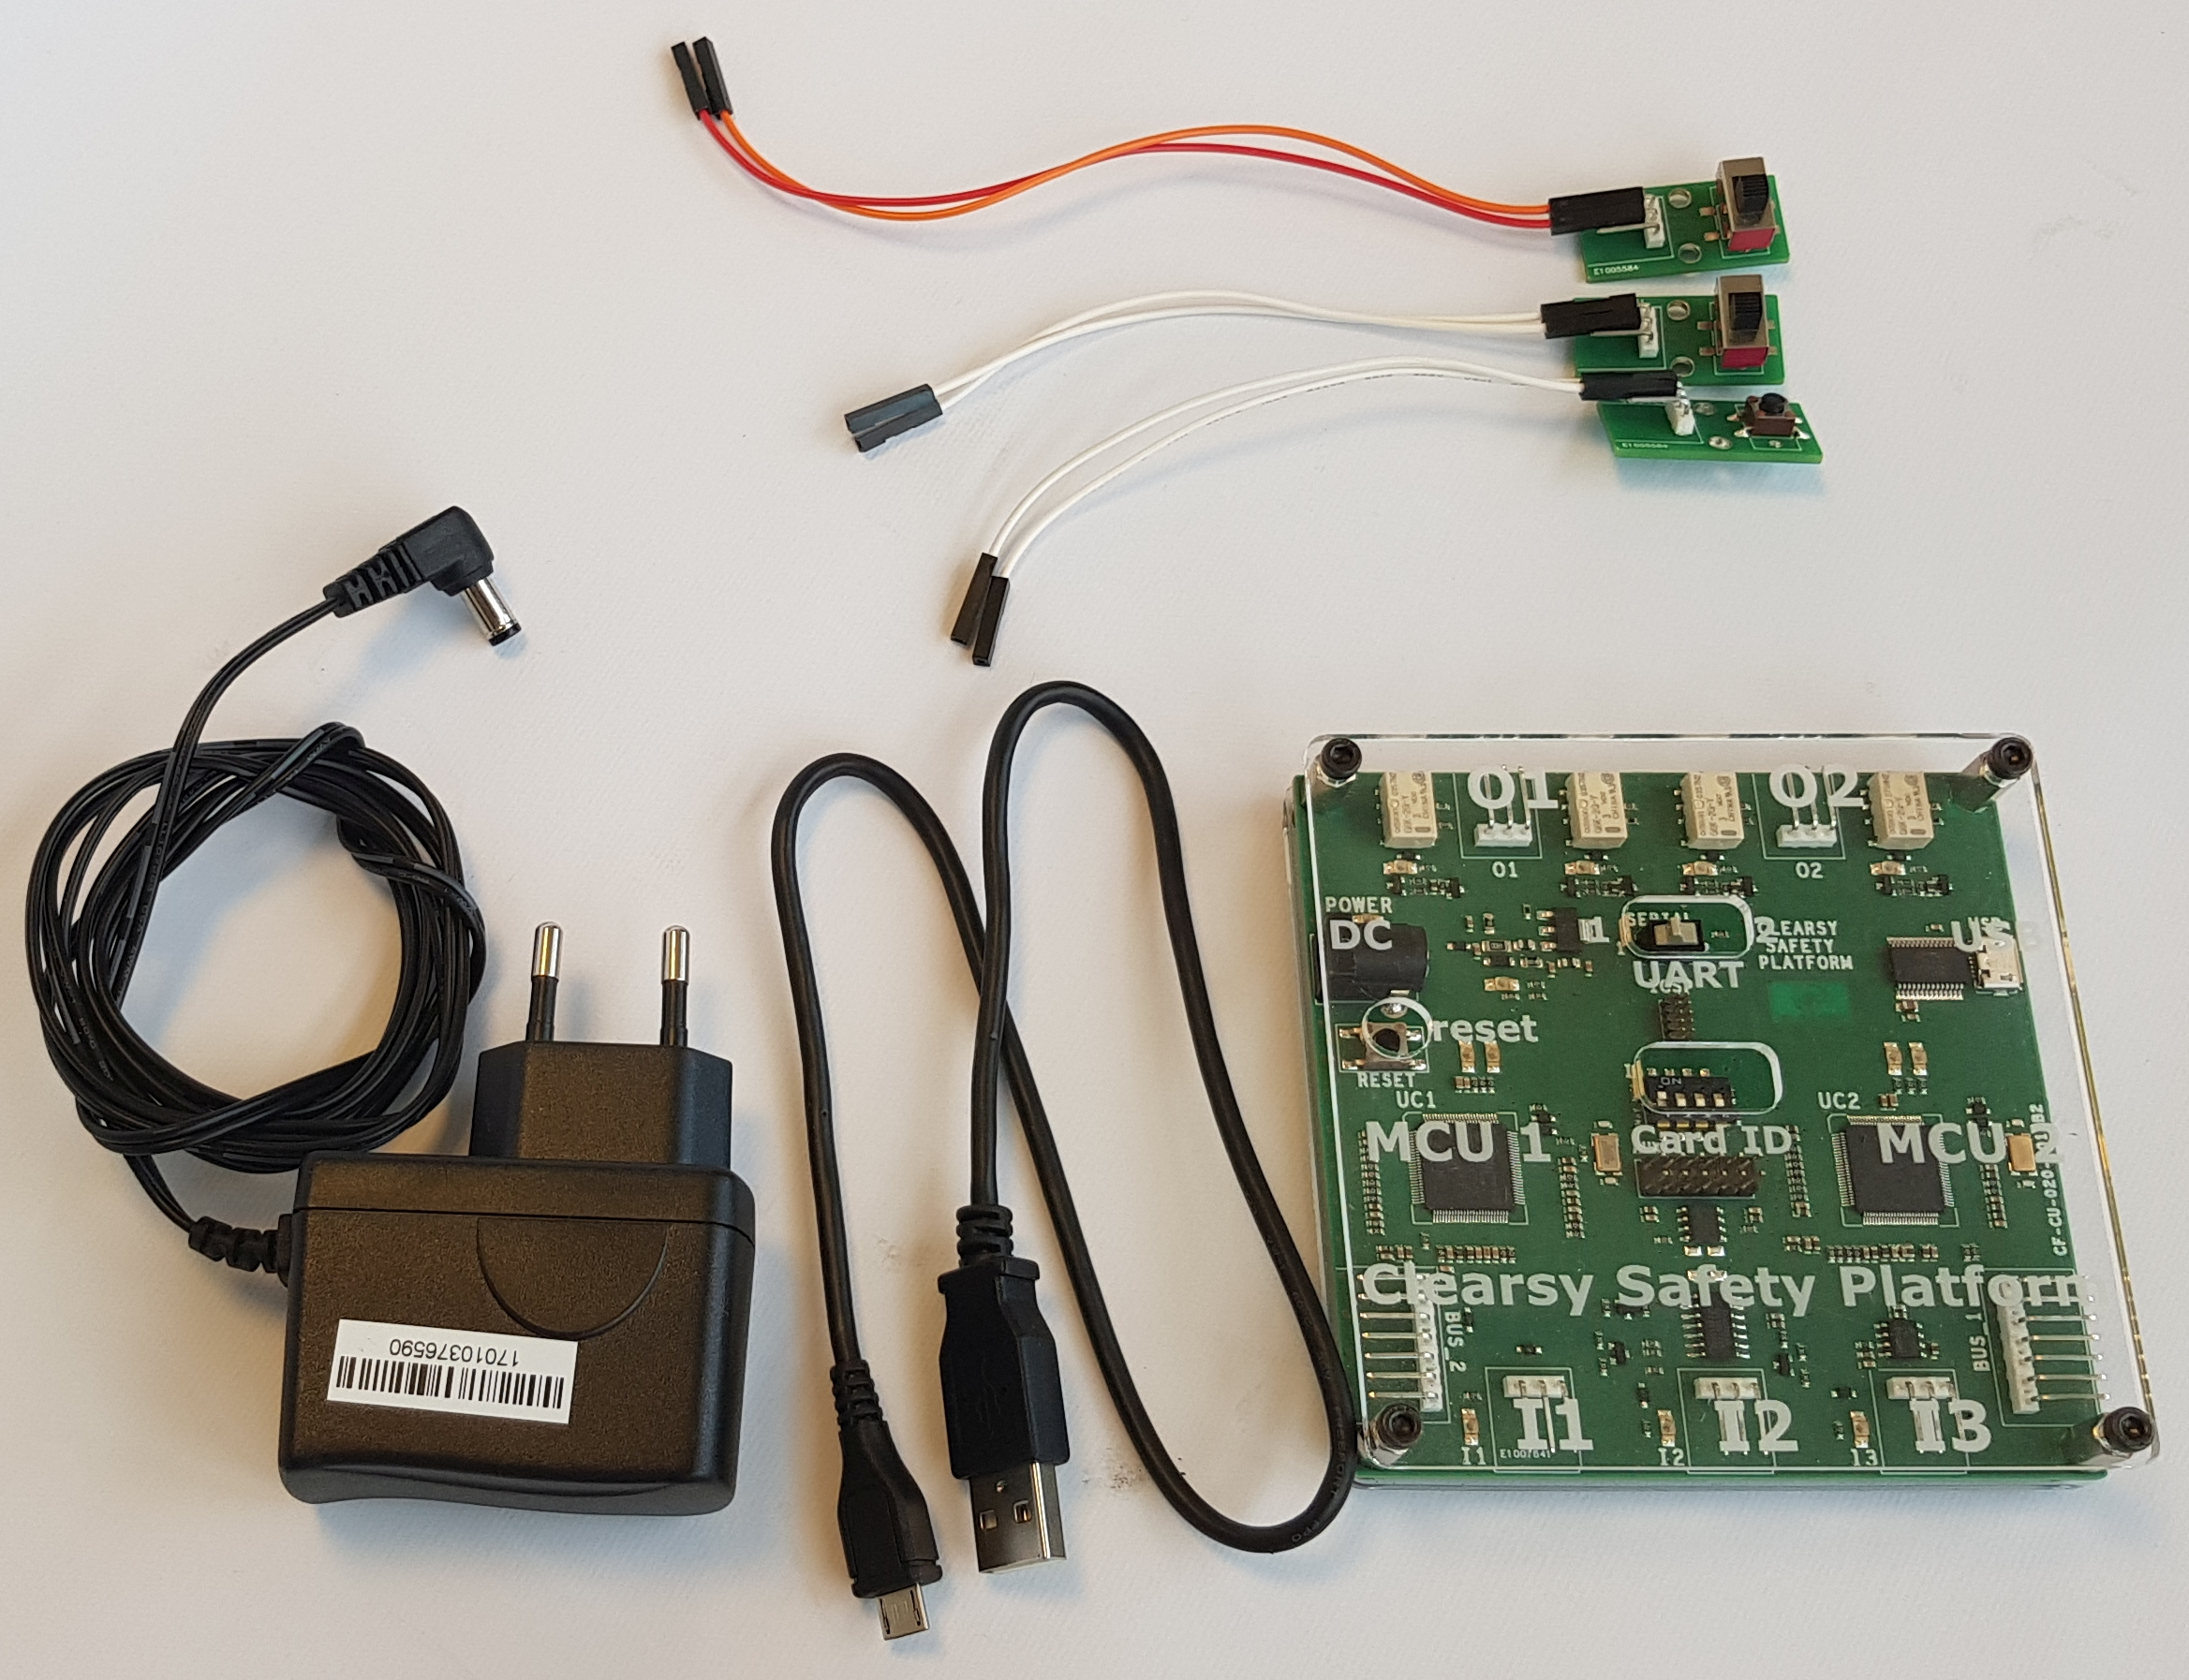
\includegraphics[scale=0.09]{Pictures/chapterProgramming/INSTALL-SK0.jpg}
\caption{The CLEARSY Safety Platform starter kit 0}
\label{install:SK0}
\end{figure}

\begin{remark}
Warning ! Do not connect the board to your PC before having completed the installation of the FTDI driver. Sometimes Windows installs another (inadequate) driver that prevents any further communication with the board. Then removing this driver is mandatory before installing the FTDI driver.
\end{remark}

The installation of the development environment is as follow:
\begin{itemize}
    \item download the installer file containing the IDE \footnote{When you buy a CSSP starter kit, you receive by email a link to download the IDE.}. The file is around 0.4 GB. 
    \item execute the installer and install it to a directory. It requires 3 GB of free space on your hard disk.  Choose preferably a path which does not contains spaces or special characters. 
        \item install the FTDI driver. Execute the file CDM21228\_Setup.exe in the directory "Drivers \& runtime". This driver is required to emulate the CSSP serial port over USB in order to communicate with the board (upload, monitor).
\end{itemize}  

\begin{figure}[ht]
\centering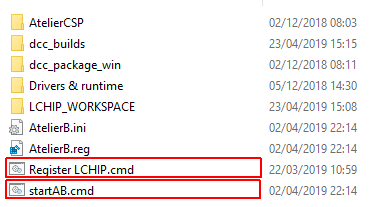
\includegraphics[scale=0.5]{Pictures/chapterProgramming/INSTALL-directory.png}
\caption{The directory where the IDE has been installed. The two scripts to use for respectively configuring and starting the IDE are highlighted in red. Register LCHIP.cmd is executed automatically during installation. startAB.cmd launches the CSSP IDE.}
\label{install:directory}
\end{figure}



\section{A first run}
During this first run, we are going to experiment with the full process of programming the CLEARSY Safety Platform. Let us start by executing the startAB.cmd script to verify that the installation has been completed. You should obtain the window shown in the figure \ref{install:ATB-window} with the two projects \textit{Clock} and \textit{Combinatorial} listed in the left pane.

\begin{figure}[h]
\centering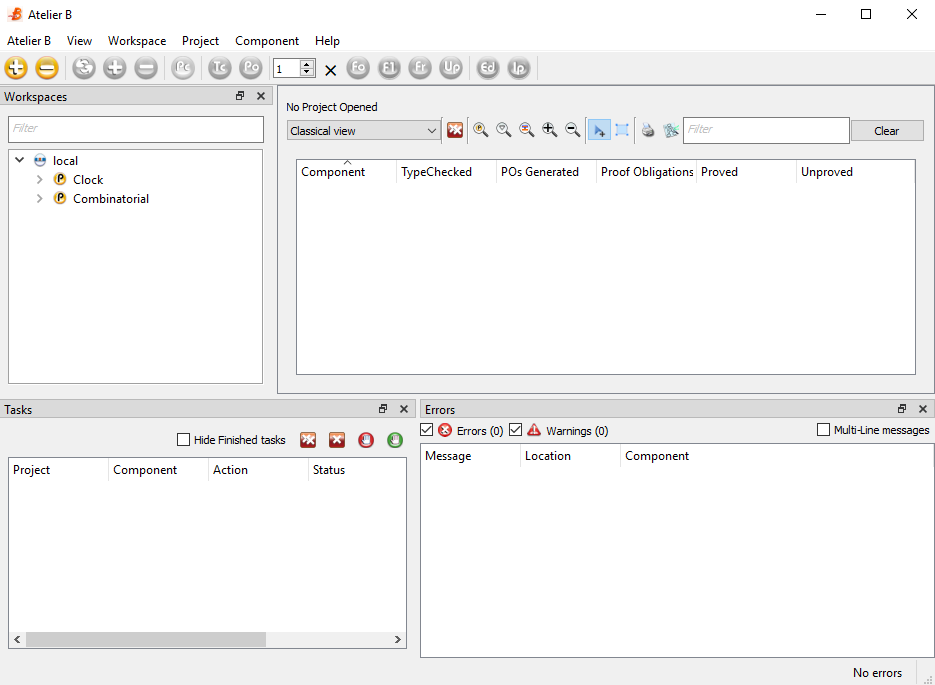
\includegraphics[scale=0.35]{Pictures/chapterProgramming/INSTALL-ATB-window.png}
\caption{The Atelier CSSP main window when executing the startAB.cmd script}
\label{install:ATB-window}
\end{figure}

\begin{remark}
\textbf{Troubleshooting}\\
If the two projects \textit{Clock} and \textit{Combinatorial} do not show up on the project list pane (left), you probably  do not have the rights to modify the Atelier B configuration files in the directory press/bdb.
\end{remark}
Power the board by using the power supply. Connect the CLEARSY Safety Platform to your PC with a micro-USB cable.  The board should now have some LEDs on after few seconds. The board is executing the program that was previously uploaded in memory. If it is the very first use of the board, the flash memory is empty and the board is literally doing nothing.\\
Let us create our first CLEARSY Safety Platform project:
\begin{itemize}
    \item go to the menu Atelier B / New / Project.
    \item select "Software development" and "Define as CSSP project" (figure \ref{install:create-project}).
    \item enter a project name that is not yet defined in the project list pane
\end{itemize}

\begin{figure}[ht]
\centering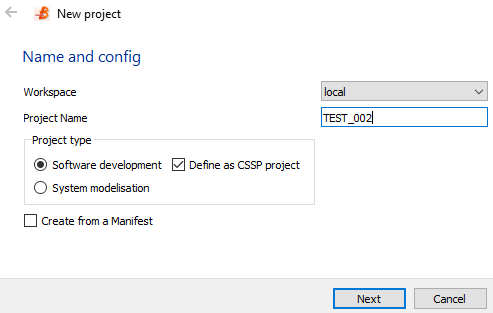
\includegraphics[scale=0.4]{Pictures/chapterProgramming/FIRSTRUN-create-project-001.png}
\caption{Information required to create a CSSP project}
\label{install:create-project}
\end{figure}

\begin{itemize}    
    \item click "Next" then "Finish".
    \item a new window requires you to select the board type - keep the default choice "SK0" and press "OK".
    \item a new window shows up to configure the number and names of the IOs.
    \item click on "create new board".
    \item a graphical representation of the board appears together with two panes on the right that allow to select the inputs to use and to edit their default name (figure \ref{install:configure-board}).
\end{itemize}
  
  \begin{figure}[h]
\centering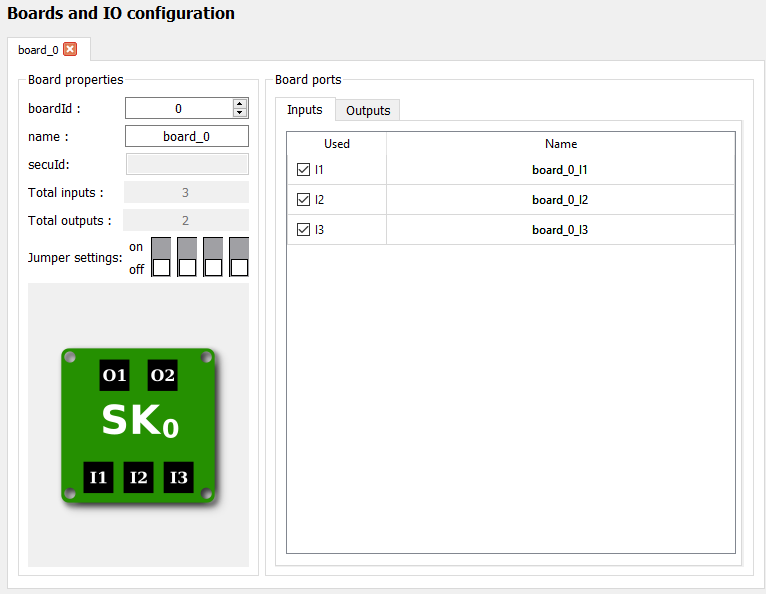
\includegraphics[scale=0.3]{Pictures/chapterProgramming/FIRSTRUN-create-project-004.png}
\caption{The configuration window to select the inputs/outputs and to modify the default naming}
\label{install:configure-board}
\end{figure}  
    
\begin{itemize}
    \item once your are happy with the configuration, click "Next".
    \item a summary page is displayed with the exact configuration of the board.
    \item click on "Finish" - you are asked to confirm the writing of the configuration. As we are creating the project, there is no previous configuration, so we can safely save it. Click on "Yes".
    \item the components of the project are generated in few seconds.
    \item then you finally get several orange boxes in the main window. The boxes represent the components generated from the configuration (IOs numbers and names). The colour represents their proof status: red/orange is "not proved", green is "proved" (figure \ref{install:project-components}).
 \end{itemize}
  
  \begin{figure}[h]
\centering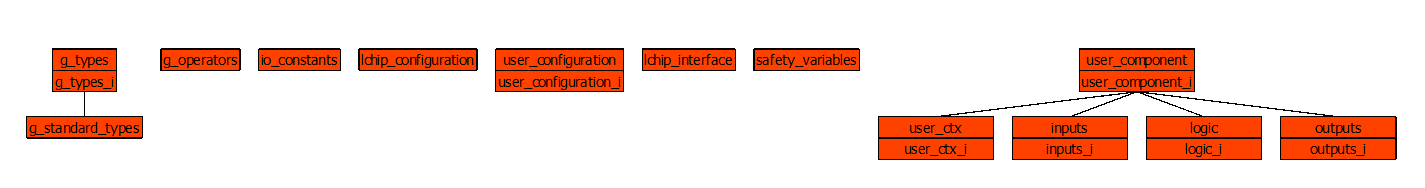
\includegraphics[scale=0.28]{Pictures/chapterProgramming/FIRSTRUN-create-project-005.png}
\caption{The CSSP project generated from the board configuration. Boxes are components.}
\label{install:project-components}
\end{figure}  
    
\begin{itemize}   
    \item select all the components with Ctrl-A.
    \item initiate their proof with Ctrl-0 (or click on the blue button "F0" on the toolbar).
    \item within 30 seconds, all the components turn to green. The project is completely proved. 
    \item now that the correctness of the project is ensured, we need to compile it. Right click on the project name (left pane) and select "CSSP Runner"\footnote{there is also a "CSSP Runner SK1" to use only with the board SK1.}.
    \item a new window - the CSSP runner - shows up, representing graphically the different stages of the compilation (figure \ref{install:cssp-runner}).
\end{itemize}
  
  \begin{figure}[ht]
\centering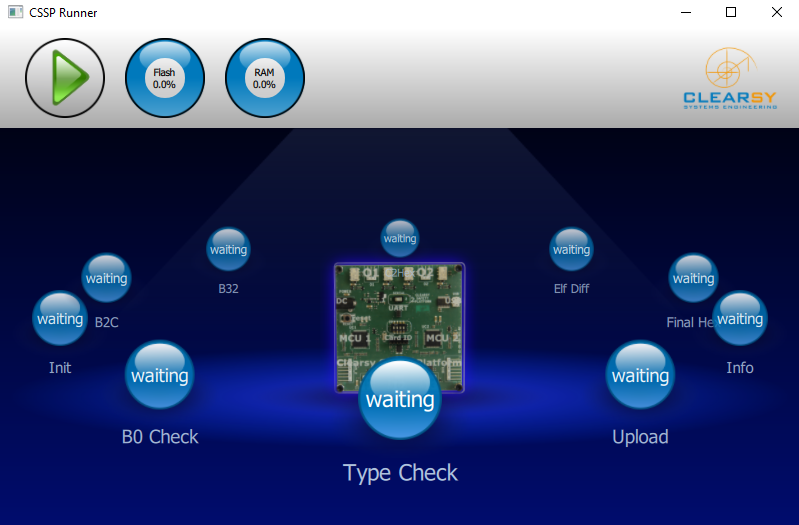
\includegraphics[scale=0.4]{Pictures/chapterProgramming/FIRSTRUN-create-project-006.png}
\caption{The CSSP runner shows the different stages of the compilation process}
\label{install:cssp-runner}
\end{figure}  
    
\begin{itemize}    
    
    \item click the green triangle on the top left to initiate the compilation
    \item an animation shows how the different stages are completed with (normally) a green tick for all of these. The memory footprint is displayed on the top during the penultimate stage. 
    \item finally the runner reaches the last stage - upload. You are asked to reset the SK0 board. Push on the reset button on the board; the board starts blinking as it enters the bootload mode \footnote{This mode is used to modify the program in flash.} and downloads the program.
    \item once the transfer is completed, you are asked to reset the board again, to leave the bootload mode. The program in flash is copied in memory then its execution is initiated.
    \item the program does nothing (no modification of the outputs): so normally you should observe the two outputs O1 and O2 of the boards set to OFF (LEDs off), and the board status LED blinking slowly. 
\end{itemize}
Congratulations! You have successfully programmed the SK0 board for the first time!

%-------------------------------------------------
\section{The programming model}

The CLEARSY Safety Platform is aimed at \textbf{automation functions for cyclic applications}, as it 
\begin{itemize}
    \item reads the digital inputs.
    \item performs computations using a subset of the B language.
    \item modifies the outputs.
    \item reads the current time since the central unit started.
\end{itemize}
The function is executed regularly as often as possible similar to Arduino programming (setup(), loop()). 
  \begin{figure}[ht]
\centering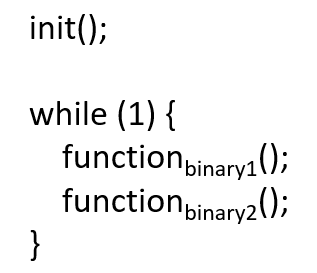
\includegraphics[scale=0.3]{Pictures/chapterProgramming/main-loop-pseudo-code.png}
\caption{The pseudo-code of the main loop}
\end{figure}  
There is no underlying operating system and no interrupt. 
There is no delay(). There is no predefined cycle time. However if the outputs are not set and cross-read every 50 ms by microcontrollers, the board SK$_0$ enters panic mode and reboots.\\
Inputs are values captured at the beginning of a cycle (instantaneous values). Input capture is synchronised on both microcontrollers in order to acquire the same values (and prevent unwanted reboot because of different behaviour over the two central units). Outputs are maintained from one cycle to another.\\

With the CLEARSY Safety Platform, the developer is incited to focus on developing a function, independently of its transformation and distributed execution. 

%-------------------------------------------------
\section{Development cycle: the steps}

The CSSP development cycle strictly follows the B method which can be summarised as:
\begin{itemize}
    \item specification model is written first, then comes the implementation model, both using the same language (B).
    \item models are proved.
    \item source code is generated from implementation models.
\end{itemize}
The whole picture (figure \ref{programming:b-method}) contains more details that are going to be explained. Fortunately the CSSP IDE helps to lower the number of actions to perform when developing an application.
  \begin{figure}[ht]
\centering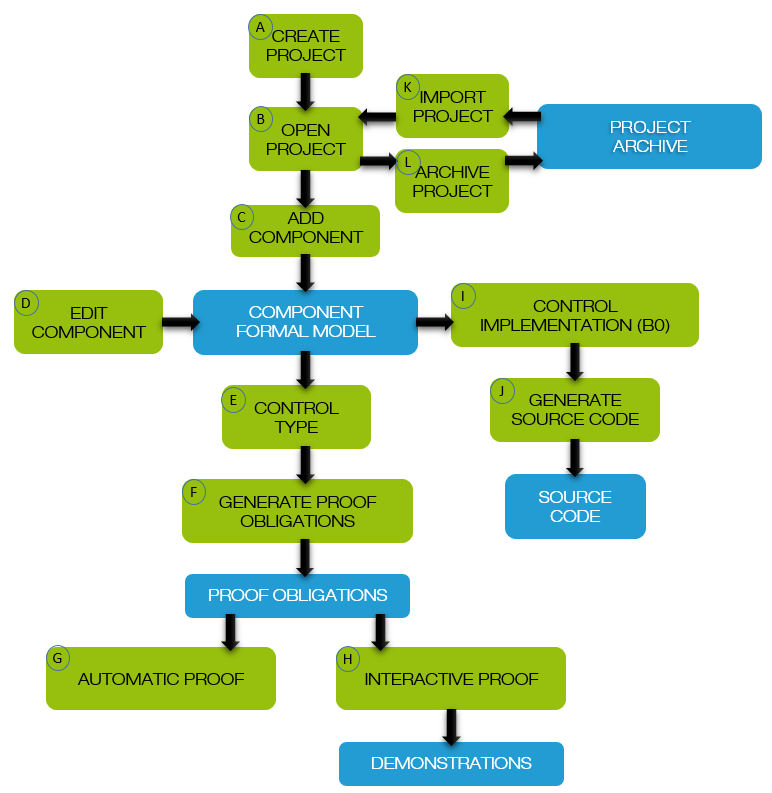
\includegraphics[scale=0.4]{Pictures/chapterProgramming/b-method.png}
\caption{The development cycle with the B method - blue boxes are files, green ones are actions performed with the CSSP IDE.}
\label{programming:b-method}
\end{figure}  

\subsection{CSSP project creation}

Creating a CSSP project\footnote{A software development project + CSSP option} covers actions \circled{A}, \circled{B}, and \circled{C}. The project is created and populated with the required components (§ \ref{annexes:interface-with-safety-library}) based on your board configuration (number and naming of inputs and outputs). There is no need to add other components for simple applications. 
\begin{remark}
It is not possible to regenerate a project once it has been created from a given configuration, in case for example you made a spelling mistake that you want to correct. As the components are automatically generated, you are going to loose all edits. Just create another project and copy/paste your edits from one project to the other.
\end{remark}

\subsection{Editing CSSP components}

Editing CSSP components covers action \circled{D}. You are entitled to modify the following components:
\begin{itemize}
    \item \textbf{user\_ctx} by 
    \begin{itemize}    
        \item adding constants (clause CONCRETE\_CONSTANTS) (optional),
        \item providing properties defining constants' types and constraints (clause PROPERTIES),
        \item adding sets (clause SETS) (optional).
    \end{itemize}   
    \item \textbf{user\_ctx\_i} by providing values to your concrete constants and sets (clause VALUES)
    \item \textbf{user\_logic} by modifying the specification of the operation user\_logic. By default, the specification is skip, meaning that all variables defined at specification level are not modified. The clauses INVARIANT and INITIALISATION could be modified as well.
    \item \textbf{user\_logic\_i} by 
    \begin{itemize}    
        \item adding variables (clause CONCRETE\_VARIABLES) (optional),
        \item adding typing properties for variables (clause INVARIANT) ,
        \item adding initialisation values for variables (clause INITIALISATION),
        \item modifying the body of the operation user\_logic (clause OPERATIONS).
    \end{itemize}   
\end{itemize}

\subsection{Proving CSSP project}

Proving CSSP project covers actions \circled{E}, \circled{F}, and \circled{G}. Initiating automatic proof by selecting one/several/all components and clicking on the "F0" button on the toolbar will start automatic proof in force 0 of these components. If required, type control and proof obligation generation are performed automatically. Your project is fully proved if all component boxes are green with graphical view or 100\% proved with classical view (figure \ref{programming:proof-status-classical}).

  \begin{figure}[ht]
\centering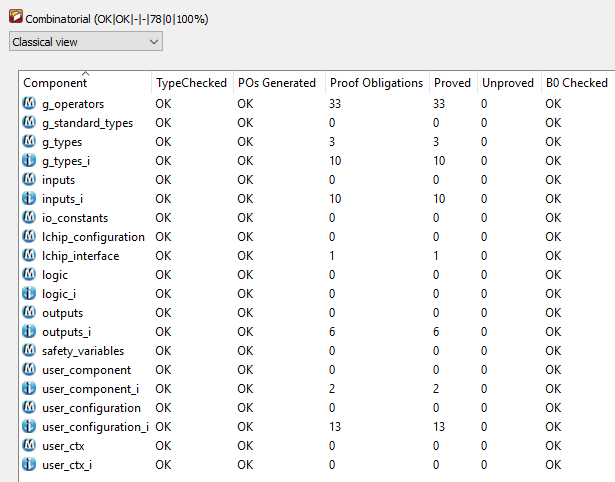
\includegraphics[scale=0.4]{Pictures/chapterProgramming/project-status-classical.png}
\caption{Proof status with classical view: 100\% proved requires to have only zeros in the "Unproved" column.}
\label{programming:proof-status-classical}
\end{figure}  

\subsection{Interactively proving  CSSP project}

Interactively proving CSSP project covers action \circled{H}. A project not fully proved automatically does not necessarily mean that the project contains errors. Unproved proof obligations might be not "adequate"/too complicated for the proof tools and require some guidance from the developer to complete the mathematical demonstration like starting a proof by contradiction or by cases, rewriting/simplifying predicates/expressions, etc. Interactive proof is an advanced topic and as such will be addressed later. 

\subsection{Generating code for CSSP project}

Generating code for CSSP project covers actions \circled{I} and \circled{J}. The CSSP Runner is triggered by selecting the project, right-clicking and then by clicking "CSSP Runner" in the drop-down menu. A new window shows up with a rotating view of the different compilation steps. After clicking the green triangle button on the top left, the different stages are executed. 
\begin{itemize}
    \item If a stage fails, you get a red cross and the compilation process stops (figure \ref{programming:runner-error}). If you click on the "error" text, you get the logs captured during the execution of the related tool. These logs may be copied by right clicking and selecting the action "copy" from the drop-down menu. 
\end{itemize}    
      \begin{figure}[h]
\centering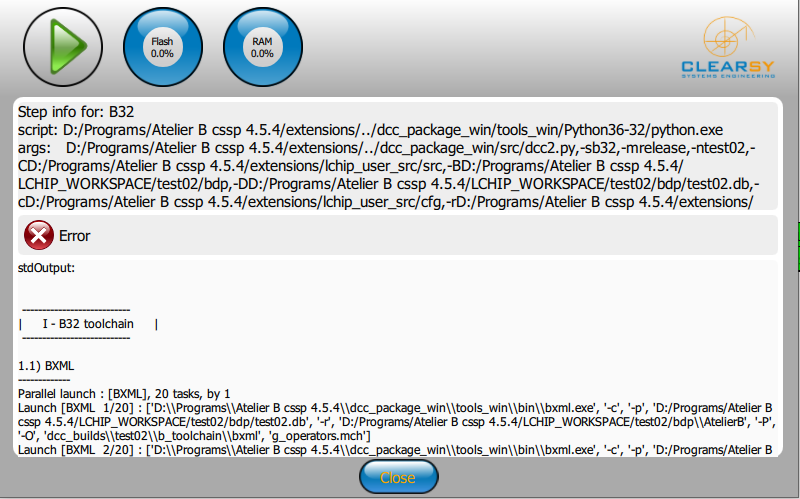
\includegraphics[scale=0.3]{Pictures/chapterProgramming/runner-error.png}
\caption{Clicking on the Error displays the logs captured during the execution of the related tool.}
\label{programming:runner-error}
\end{figure}  
\begin{itemize}
    \item If all the compilation stages succeed, you get information about the memory consumption for both Flash and RAM. Check that you do not exceed 100\%\footnote{In this case, you need to simplify your program to remain within this limit.}. You are asked to reset the board to enter bootload mode. As soon as the reset button is pushed, the two upload LEDs start blinking for around 30 seconds. Then the last stage gets a green tick and you are asked to reset again the board to leave bootload mode. Once the reset button is pressed, the board starts executing the software copied in Flash memory within 2 seconds.
\end{itemize}
      \begin{figure}[h]
\centering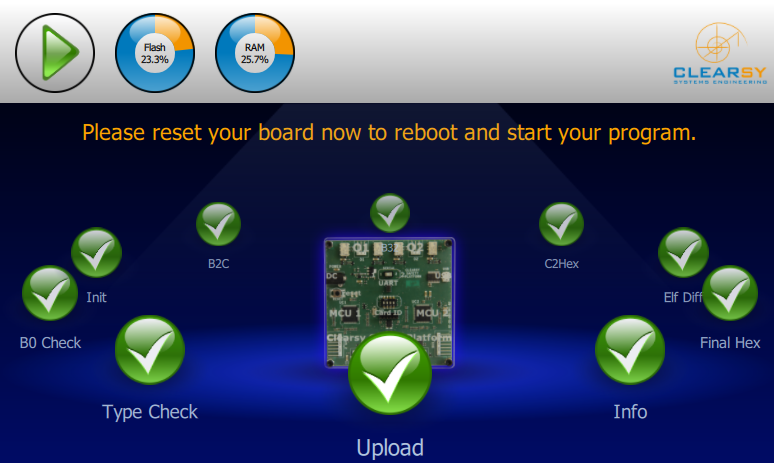
\includegraphics[scale=0.3]{Pictures/chapterProgramming/runner-upload-completed.png}
\caption{All green ticks indicate a successful compilation and upload.}
\label{programming:runner-upload-completed}
\end{figure}  

\subsection{Archiving and importing for CSSP project}

Archiving and importing for CSSP project cover actions \circled{K} and \circled{L}. To archive a project, select it, right-click and select "archive". Chose the destination directory (the archive file has the .arc extension). Chose "whole project" then "Next" and "Finish".
To import a CSSP project, select "Workspace/restore project". Click "Next". Select the archive file to you to import, give a name to the project and click "Next" then "Finish". A new project appears in the left pane, with the contents of the archived project.

%-------------------------------------------------
\section{Programming the board}

Programming the board (figure \ref{programming:all})  consists of:
\begin{itemize}
    \item describing, in the component \textit{logic}, the behaviour of the board,
    \item declaring and using constants, defined in the component \textit{user\_ctx},
    \item reusing operations defined in the component \textit{inputs} and in the safety library.
\end{itemize}
\begin{figure}[ht]
\centering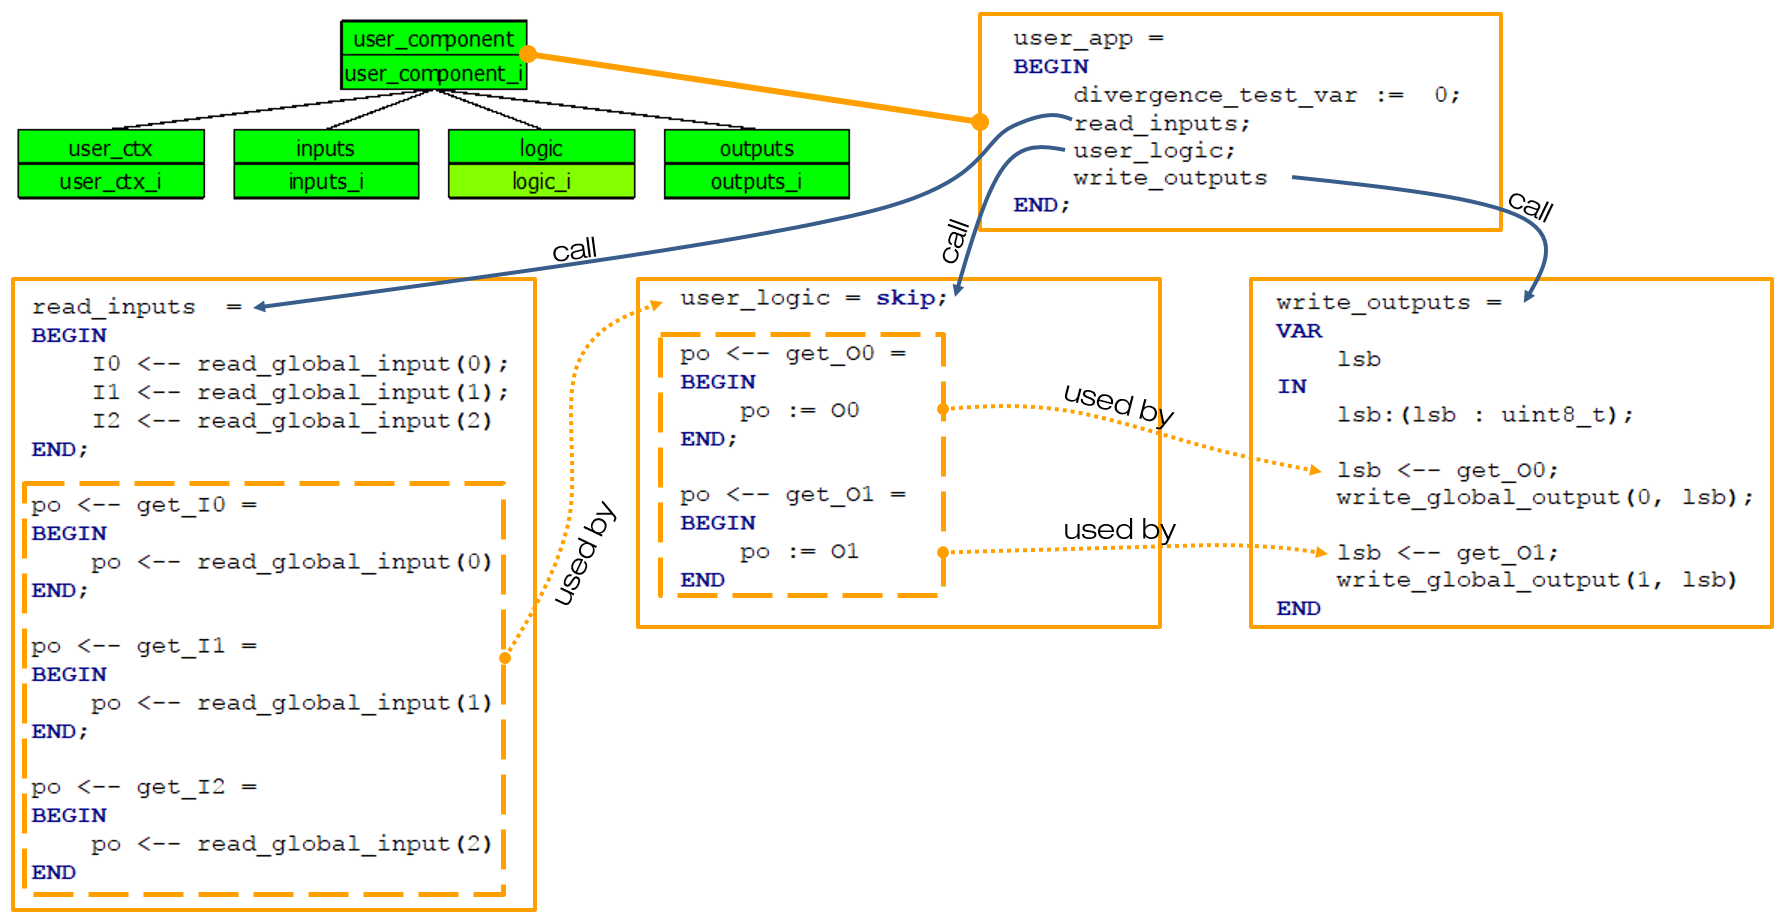
\includegraphics[scale=0.25]{Pictures/chapterProgramming/programming-all.png}
\caption{The default CSSP project showing the dependencies between the components. }
\label{programming:all}
\end{figure} 
All the operations defined in the components \textit{inputs} and \textit{outputs} have to remain unchanged, as well as the accessing functions get\_* defined in the component \textit{logic}.\\
The structure of the component \textit{logic} is seen in figure \ref{programming:spec}. It contains several clauses:
\begin{itemize}
    \item SEES: contains the list of all seen components.
    \item ABSTRACT\_VARIABLES: the outputs of the board. They are going to be refined in CONCRETE\_VARIABLES (implementable) in the component \textit{logic\_i}.
    \item INVARIANT: the type of the variables, with some constraints between them (optional).
    \item INITIALISATION: the first value assigned to the variables. At specification level, initialisation may be non-deterministic (any value complying with some conditions).
    \item OPERATIONS: each operation specifies how the modelling variables are modified, preferably without the algorithmic details.
\end{itemize}
\begin{figure}[ht]
\centering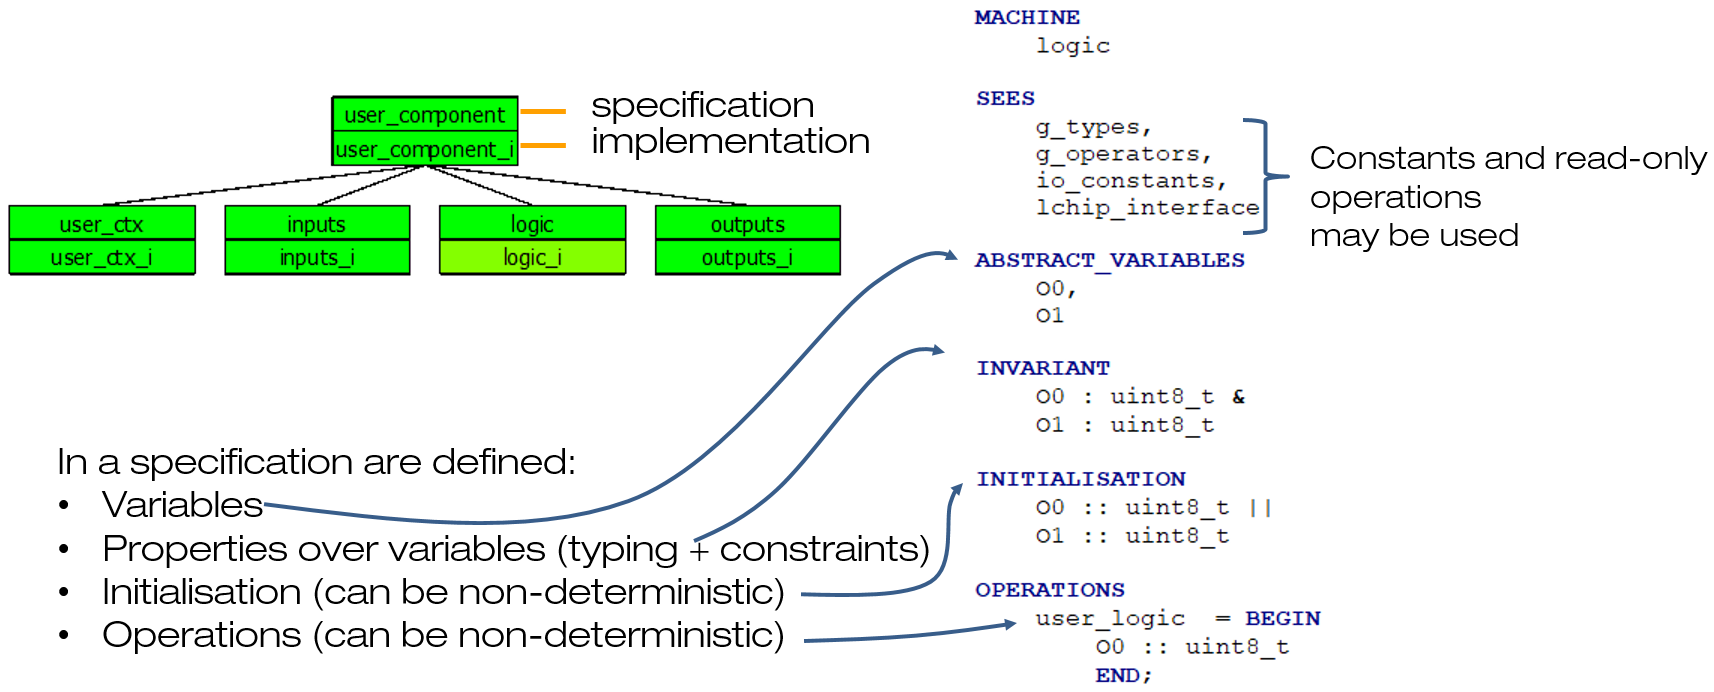
\includegraphics[scale=0.25]{Pictures/chapterProgramming/programming-spec.png}
\caption{The structure of the logic component (specification).}
\label{programming:spec}
\end{figure}
Once the specification component has been modified\footnote{It should mention \textit{a minima} that the outputs are going to be modified when the operation user\_logic is executed.}, it is time to modify the component \textit{logic\_i}. 
The structure of the component \textit{logic\_i} (figure \ref{programming:implem}) is quite similar to that of component \textit{logic}:
\begin{itemize}
    \item SEES: the implementation should see the same components.
    \item CONCRETE\_VARIABLES: outputs variables have to be concrete (implementable). New variables (not defined in the component \textit{logic}) could be added.
    \item INVARIANT: a concrete type (uint8\_t, uint16\_t, uint32\_t, or BOOL) has to be given to all concrete variables declared. Board outputs must be declared as uint8\_t.
    \item INITIALISATION: all variables have to be assigned a deterministic value. This value should comply with its type.
    \item OPERATIONS: the behaviour of each operation has to be implemented with only implementable substitutions.
\end{itemize}
\begin{figure}[ht]
\centering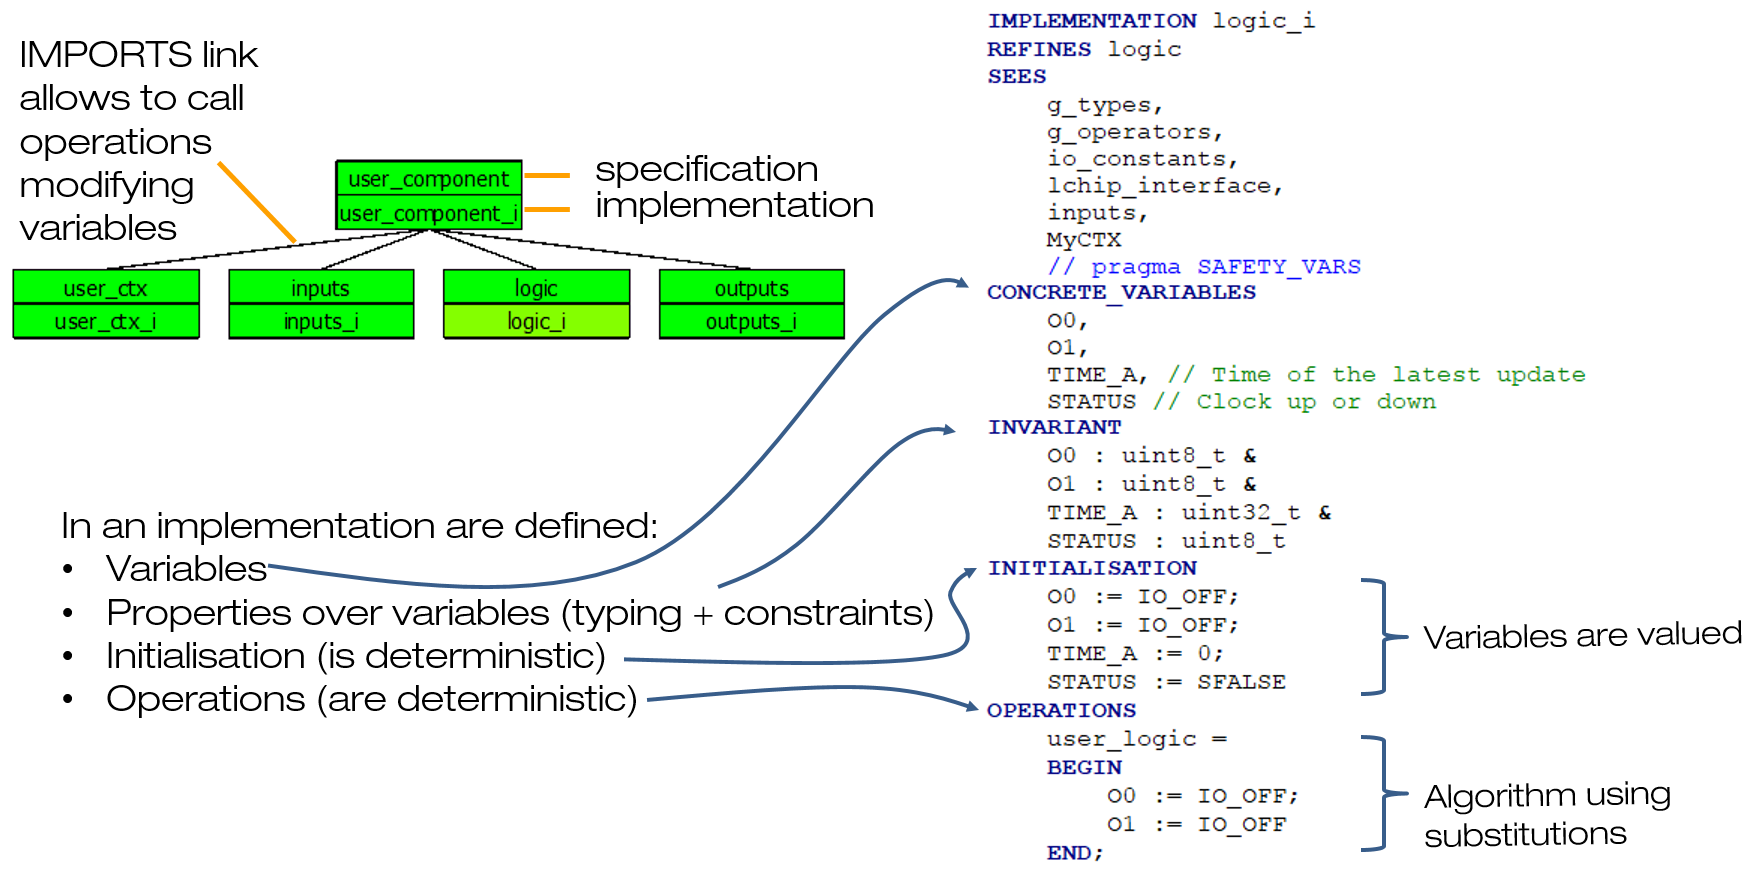
\includegraphics[scale=0.25]{Pictures/chapterProgramming/programming-implem.png}
\caption{The structure of the logic\_i component (implementation).}
\label{programming:implem}
\end{figure}  

%------------------------------------
\subsection{Declaring variables}

Figure \ref{programming:var-decl} shows how variables are declared side-by-side in specification and implementation:
\begin{itemize}
    \item first goes a list of variables, either abstract or concrete, separated by commas.
    \item in the implementation, the pragma SAFETY\_VARS is mandatory to indicate that the implementation contains variables that need to be managed by the safety library.
    \item the invariant contains a list of predicates, separated by \&, where types and constraints are expressed. Types in implementation are only implementable types.
    \item the initialisation describes the initial value of the variables. In the specification, the initialisation may be deterministic or non-deterministic. In the implementation, the initialisation has to be deterministic and to comply with the one in the specification\footnote{If "vv belongs to uint16\_t" was the initialisation of the variable vv, then "vv := 0" is a correct initialisation in implementation, while "vv := -1" is not.}. Moreover initialisations in specification are performed "in parallel" by using the operator ||; in implementation, initialisations are ordered by using the operator ; (sequence).
\end{itemize}
\begin{figure}[ht]
\centering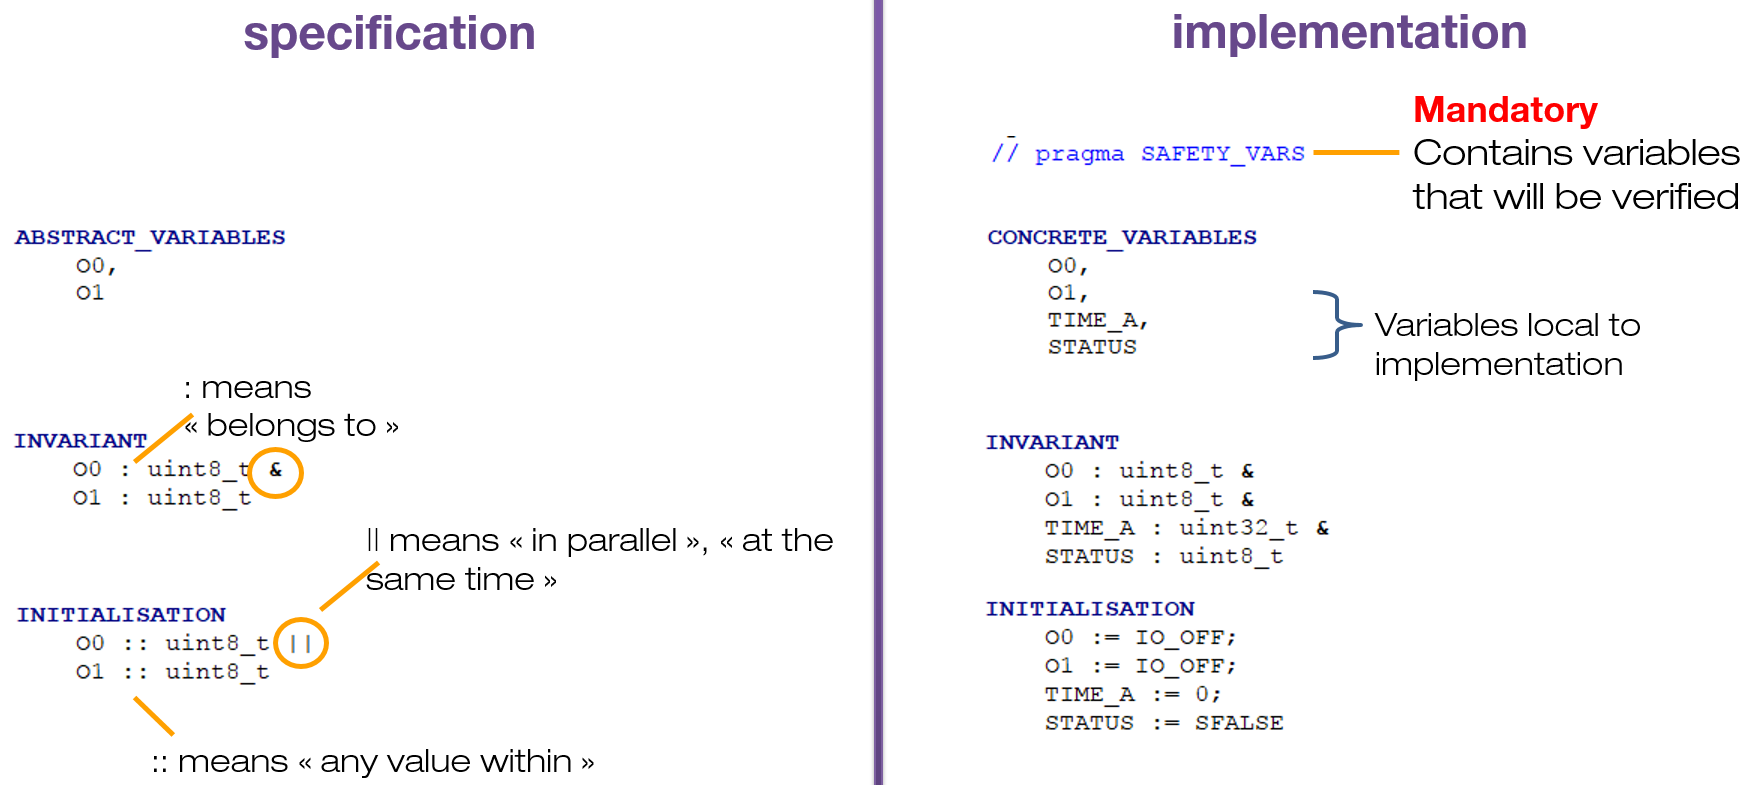
\includegraphics[scale=0.25]{Pictures/chapterProgramming/variables-decl.png}
\caption{Declaring variables in specification and implementation.}
\label{programming:var-decl}
\end{figure}  

%------------------------------------
\subsection{Declaring constants}

Figure \ref{programming:constant-decl} shows how constants are declared side-by-side in specification and implementation:
\begin{itemize}
    \item first goes a list of constants, either abstract or concrete, separated by commas.
    \item in the implementation, the pragma CONSTANTS is mandatory to indicate that the implementation contains constants that need to be managed by the safety library.
    \item in the specification, the PROPERTIES contains a list of predicates, separated by \&, where are expressed types and constraints. Properties are only in specification.
    \item in the implementation, the VALUES sets the value of the constants. Values provided have to comply with constant properties.
\end{itemize}
\begin{figure}[ht]
\centering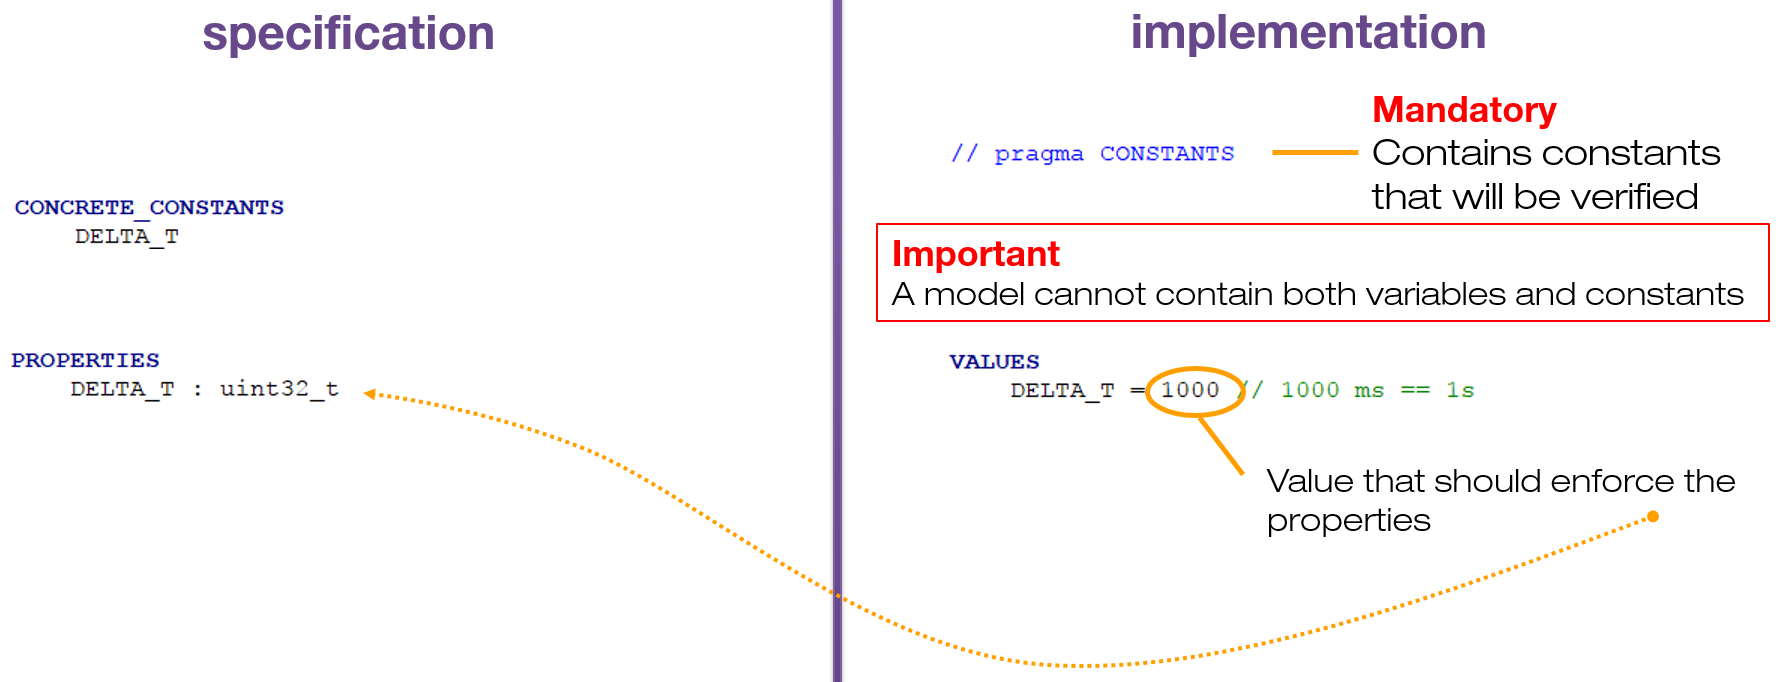
\includegraphics[scale=0.25]{Pictures/chapterProgramming/constants-decl.png}
\caption{Declaring constants in specification and implementation. }
\label{programming:constant-decl}
\end{figure}  

\begin{remark}
An implementation should contain one and only one pragma: either SAFETY\_VARS or CONSTANTS. That is why two components are made available: \textit{user\_ctx} for hosting constants and \textit{logic} for variables and behaviour.
\end{remark}

%------------------------------------
\subsection{Describing a behaviour}

Behaviour is described in OPERATIONS. Operations are populated with substitutions. Substitutions allow to describe how variables are (conditionally) modified. Available substitutions in specification are different from the ones available in implementation. We are going to see a number of these in what follows.

\subsubsection{Specification}

In specification, substitutions express the properties that the variables comply with  when the operation is completed independently from  the algorithm implemented\footnote{By using post-condition: the properties that are true when the substitution has been executed.}. A good practice is to systematically use the substitution "becomes such that" (Figure \ref{programming:subst-becomes-such-that}).\\ A simple general form of the substitution is 
\begin{center}
\textit{var : (var : type(var))}    
\end{center} where \textit{var} is an identifier and \textit{type(var)} is a set expression compatible with the type of the variable \textit{var}. It could  also be of the form:
\begin{center}
\textit{var\_list : (predicate\_list)}    
\end{center} where \textit{var\_list} is a list of identifiers separated by commas and \textit{predicate\_list} is conjunction of predicates separated by \&.
\begin{figure}[ht]
\centering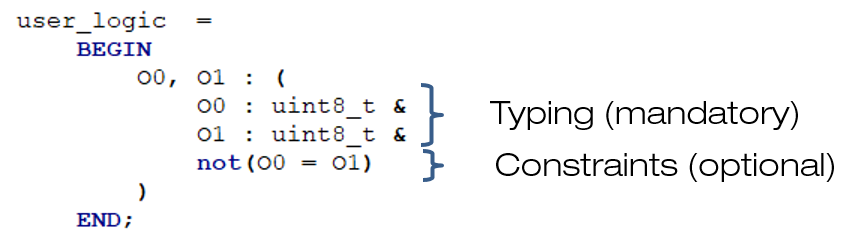
\includegraphics[scale=0.30]{Pictures/chapterProgramming/subst-becomes-such-that.png}
\caption{The substitution "becomes such that" used to specify that O0 and O1 are going to be modified within their type such that O0 is different from O1. }
\label{programming:subst-becomes-such-that}
\end{figure}  
Of course, if the value assigned to a variable is well-known, it is also possible to use the valuation substitution with:
\begin{center}
\textit{var := value}    
\end{center} where \textit{value} is a either a constant name, another variable identifier, a Boolean or an Integer value.\\

If none of the variables is going to be modified then use the substitution \textit{skip}.\\

\subsubsection{Implementation}

In implementation, several substitutions are available. Some of these are shown in figure \ref{programming:subst-implem}.

\begin{figure}[ht]
\centering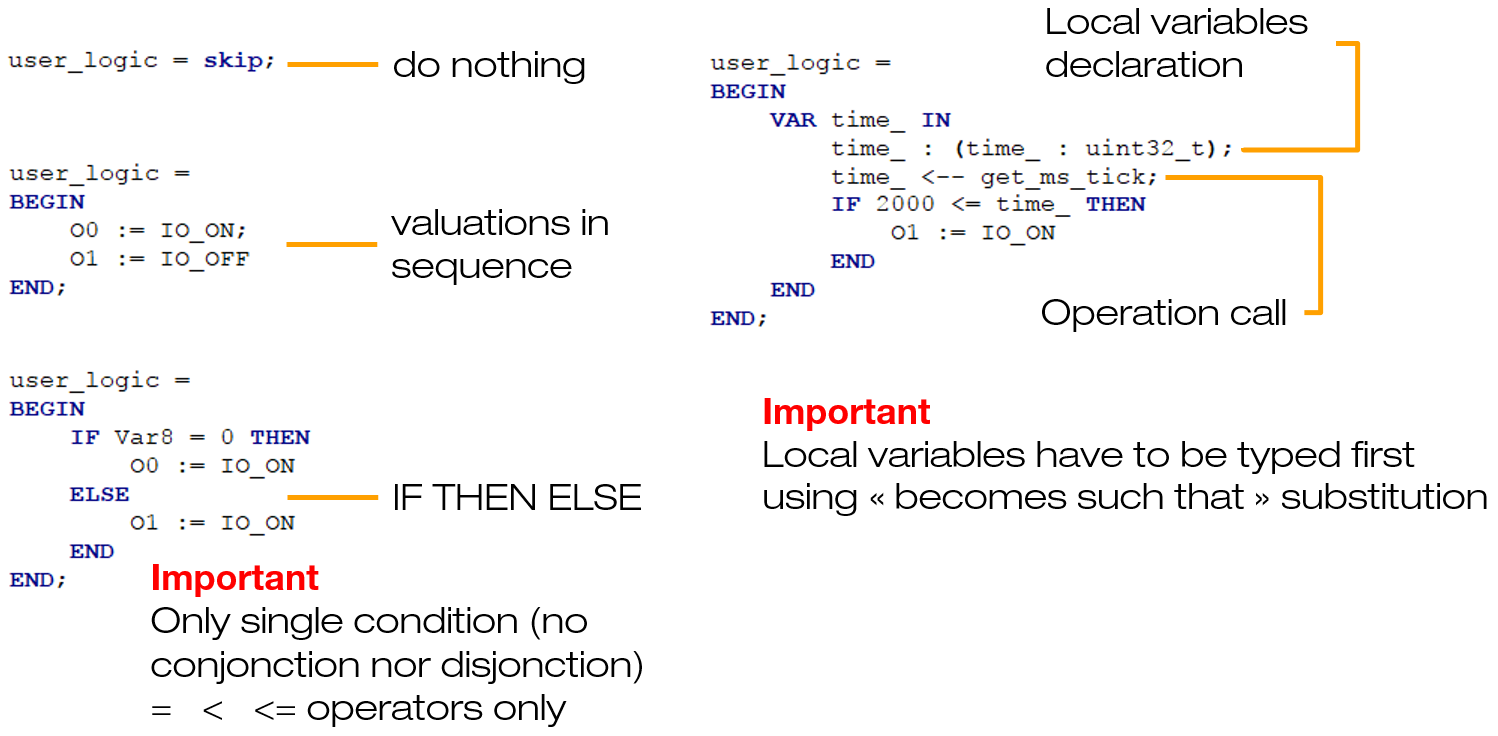
\includegraphics[scale=0.30]{Pictures/chapterProgramming/subst-implem.png}
\caption{Some substitutions usable in implementation. }
\label{programming:subst-implem}
\end{figure}  

\begin{itemize}
    \item the \textit{skip} substitution, when the variables are not modified.
    \item the assignment substitution \textit{var := value}.
    \item the sequence substitution ; to order substitutions.
    \item the IF-THEN-ELSE substitution. Only a single condition is accepted. If several conditions have to be verified, several IF-THEN-ELSE substitutions have to be nested. Testing conditions have to be simple, hence computations have to be performed independently from (before) the test\footnote{For example, it is not possible to write IF xx+1<=yy THEN skip END. Instead a local variable has to be declared and used to compute xx+1. The test is then performed with this local variable.}
    \item the local variable substitution \textit{VAR var IN substitutions END}. Local variables are used to store data and results of computation. Before any use of a local variable a substitution "becomes such that" has to be used to give a type to this local variable.
    \item the operation call substitution \textit{var\_list <-- operation(var\_list)} which use 0..n input parameters and 0..n return parameters.
\end{itemize}
These substitutions may be used in combination to obtain the final algorithm. The loop substitution will be introduced later on, in the projects.

\subsubsection{Reconciling specification and implementation}

If the writing of an implementation is quite straightforward, especially when the logic is not too complicated, the writing of a specification is far more complex. 
\begin{figure}[ht]
\centering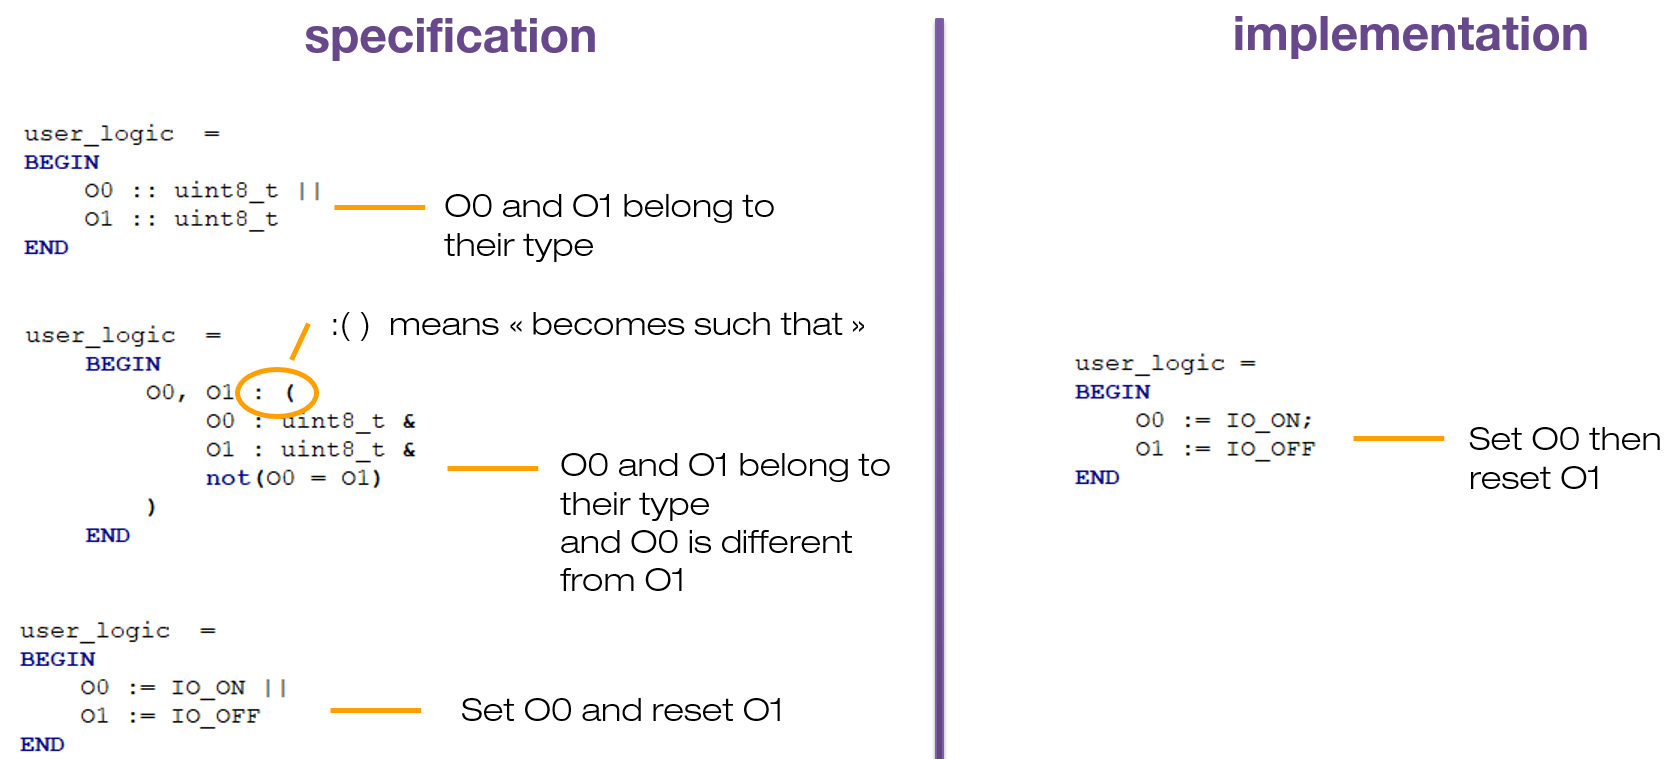
\includegraphics[scale=0.30]{Pictures/chapterProgramming/subst-reconcile.png}
\caption{Several specification compatible with the implementation. }
\label{programming:subst-reconcile}
\end{figure}  
For example, the figure \ref{programming:subst-reconcile} shows three different kinds of specification:
\begin{itemize}
    \item the first one is fully non-deterministic. If one mistake is inserted in the implementation (both values at IO\_OFF for example), it is not detected by the proof.
    \item the second one is non-deterministic but ensures that both values for O0 and O1 are different. Errors are detected except if the implementation is the contrary of what it should be.
    \item the last one is fully deterministic but very close to the implementation. One risk when having such close specification/implementation is that we are only proving the copy/paste action between both models.
\end{itemize}
It is up to you to determine what kind of specification and more importantly what level of verification you are looking for. If your model only contains loosely constrained specification, the proof will not improve much the level of confidence in the algorithm.



%=======================================================================
%	PART II: EXAMPLES
%=======================================================================
\part{Projects}

%---------------------------------------------------------------------
%	Chapter Combinatorial
%---------------------------------------------------------------------
\chapterimage{back2.jpg} % Chapter heading image
\chapter{Combinatorial}

This first project introduces the combinatorial or asynchronous behaviour of the board. The outputs are updated as soon as the inputs are modified and not after a given period of time (a delay) which is a synchronous behaviour.\\
The equations that we would like to implement are:
\begin{center}
O$_0$ = I$_1$ and I$_2$ and I$_3$\\
O$_2$ = not(O$_1$)    
\end{center}
O$_1$ will be ON only when all inputs are ON, unless it will be OFF (the AND function over three Boolean values). 0$_2$ is the opposite of O$_1$: 0$_2$ is ON when O$_1$ is OFF, and OFF when O$_1$ is ON \footnote{This is a usual practice in the railways to detect if an equipment is failing or has not power supply. If both outputs are OFF, we know that the system is failing and the situation has to be handled with care.}.

\section{Modelling}

The modelling requires three steps:
\begin{itemize}
    \item The first step is to create a project, to give it a name and select "CSSP project".
    \item The second step is to add a board (only one) and to change the names of the inputs and outputs to respectively I1, I2, I3 and O1, O2.
    \item the third step is to modify the components \textit{logic} and \textit{logic\_i} to specify and implement the behaviour. 
\end{itemize}
 
 \lstset{frameround=fttt,keywordstyle=\color{ocre}\bfseries}
\lstinputlisting[language=B, frame=trbl, firstline=19,lastline=23,caption={Non-deterministic specification of the operation user\_logic},label=examples:combinatorial-spec, rulecolor=\color{ocre}]{chapterProjects/combinatorial_1_logic.mch}

For \textit{logic}, we need to modify the specification of the operation user\_logic. We could be precise and express directly the relationship between inputs and outputs, but for the very first experiment, we prefer to simply assert that the two outputs O1 and O2 are going to be modified non-deterministically\footnote{The var :: type substitution is called non-deterministic because particular value is provided. In the implementation, the value assigned to the variable var should belong to uint8\_t. We remind you that the input and output digital values are represented by 8-bit values: IO\_OFF and IO\_ON.} (see listing \ref{examples:combinatorial-spec}). 

 \lstset{frameround=fttt,keywordstyle=\color{ocre}\bfseries}
\lstinputlisting[language=B, frame=trbl, firstline=24,lastline=49,caption={The implementation of the operation user\_logic},label=examples:combinatorial-impl, rulecolor=\color{ocre}]{chapterProjects/combinatorial_1_logic_i.imp}

For \textit{logic\_i}, the variables 01 and 02 are already defined as CONCRETE\\VARIABLES and both initialised with the value IO\_OFF. No other variable is required for the implementation. We only need to modify the body of the operation user\_logic (see listing \ref{examples:combinatorial-impl}). \\
We need three local variables to store the values of the three inputs I1, I2 and I3. So we define three variables i1\_, i2\_ and i3\_ with the substitution VAR ... IN ... END. The scope of this substitution in the END keyword, meaning that any use of these three variables outside of this scope will produce an error message. These three variables are typed prior to any use, by using the "becomes such that" substitution with the type uint8\_t. These three typing substitutions have no effect on the modelling but are required by the compiler.\\
The values of the inputs is collected by calling the three operations get\_I1, get\_I2 and get\_I3. The notation "var <-- op" means that the operation op is called and return one value that is assigned to the variable var. In our case, i1\_, i2\_ and i3\_ are valued respectively with the values returned by get\_I1, get\_I2 and get\_I3.
The next 8 lines represent the computation of O1: O1 is first set to IO\_OFF and then set to IO\_ON only if the three inputs are all equal to IO\_ON. 
\begin{remark}
The compiler in it current version does not support multiple testing conditions. Hence IF THEN ELSE have to be nested. 
\end{remark}
Finally O2 is computed with the last IF THEN ELSE, based on the value computed for O1.
\begin{remark}
The sequence operator ; is not a line terminator like in C. Its role inside an operation\footnote{It is also used to separate operations} is to separate two substitutions. If extra ; are inserted in the model, error messages will be emitted when checking the model. 
\end{remark}

\section{Executing}

Now that the modelling is complete, we first need to check and prove the model. Select all the components by clicking on the central pane of the main window\footnote{the one showing all the components of the project.}, then type ctrl+A. Type ctrl+0 to initiate the typecheck, proof obligation generation and proof of all these components. If some mistake was made, error messages are displayed either in the model editor or the error/warning pane in the main window. Be sure to correct any mistake before moving on. Finally press ctrl+U to complete the proof. You should obtain the proof status of the figure \ref{projects:Combinatorial_1-project-status} (the Unproved column shows only zeros, meaning that the project is fully proved).
\begin{figure}[h]
\centering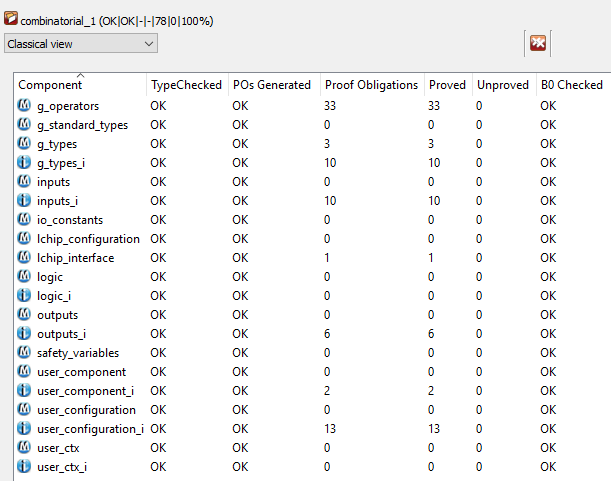
\includegraphics[scale=0.5]{Pictures/chaptProjects/comb1-project-status.png}
\caption{Combinatorial\_1 project status}
\label{projects:Combinatorial_1-project-status}
\end{figure}
The project is ready to be compiled. Be sure that your SK0 board is connected with the USB connector to your host. Right-click on the project name in the left pane and select "CSSP Runner". A new window appears, showing a carousel of all the steps of the compilation. Click on the green triangle on the top left. All steps are cleared until the last one where you are asked to reset the SK0 board. Use a pen to push on the reset button and release it. The board starts to blink as it enters bootload mode. After around 30s, the last step is cleared (green check) and you are again invited to reset the SK0 board. Push the reset button and release it. After 2 seconds, the board starts to execute your program.

\section{Testing}

To test your program, you need to be able to modify the status of the inputs in order to change the status of the outputs. You need three switches or three wires that you could plug/unplug to open/close the input circuits. The switches have to be connected to the two right pins as shown on figure \ref{projects:Combinatorial_1-connecting}.
\begin{figure}[h]
\centering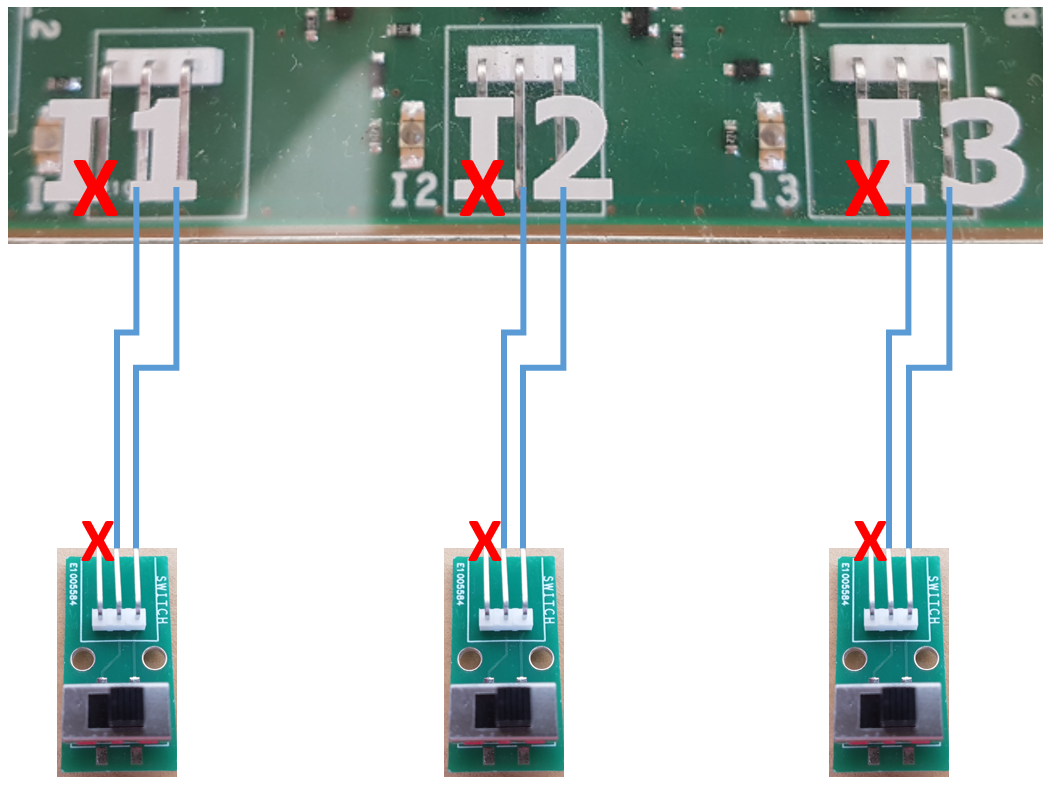
\includegraphics[scale=0.25]{Pictures/chaptProjects/combinatorial-montage.png}
\caption{Connecting switches to the board}
\label{projects:Combinatorial_1-connecting}
\end{figure}
The status of the three inputs is indicated by three LEDs. One LED is ON when enough current is provided through the input circuit, OFF if not. \\
Connect your switches, change their status and see how the behaviour evolves. You should get the configurations shown in figure \ref{projects:Combinatorial_1-connecting}.
\begin{figure}[h]
\centering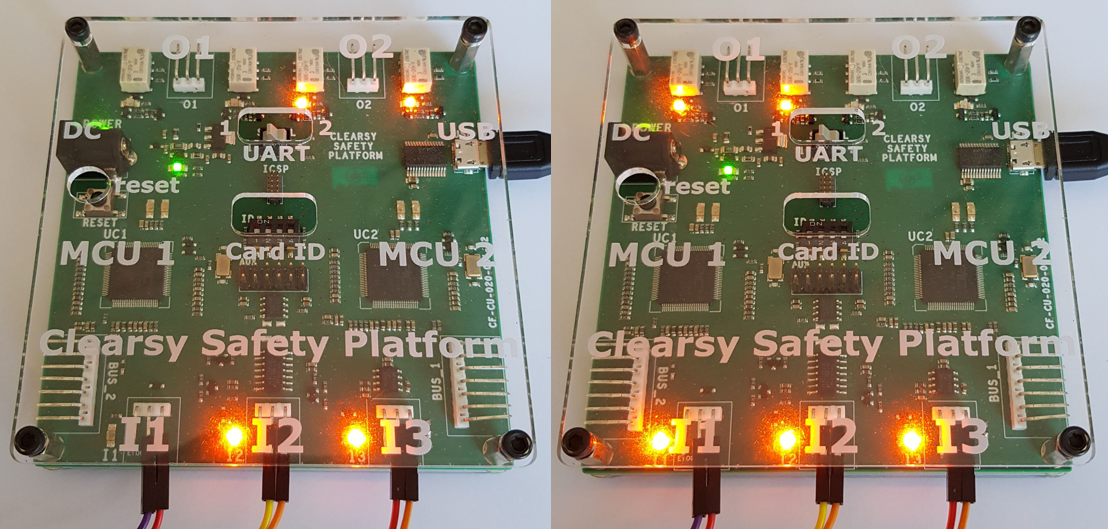
\includegraphics[scale=0.5]{Pictures/chaptProjects/comb1_join.png}
\caption{Two configurations: not all inputs are ON (left) and only O2 is ON; all inputs are ON (right) and only O1 is ON.}
\label{projects:Combinatorial_1-connecting}
\end{figure}

\begin{exercise}
Create a program which implements the following equations:
\begin{center}
O$_0$ = I$_1$ or I$_2$ or I$_3$\\
O$_2$ = not(O$_1$)    
\end{center}
First create a new project and populate it with models similar to combinatorial\_1. Then modify the body of the operation user\_logic in the component \textit{logic\_i} to implement a disjunction over the values of the three inputs.
\end{exercise}

%---------------------------------------------------------------------
%	Chapter Clock
%---------------------------------------------------------------------
\chapterimage{back2.jpg} % Chapter heading image
\chapter{Clock}

This second project introduces the synchronous behaviour of the board. The outputs are updated regularly after a given period of time (a delay).\\
The equations that we would like to implement are:
\begin{center}
O$_1$ = not(O$_1$) every second (synchronous)\\
O$_2$ = not(O$_2$) all the time (asynchronous) 
\end{center}
O$_1$ changes its status every second between OFF and ON. 0$_2$ is the opposite of O$_1$: 0$_2$ is ON when O$_1$ is OFF, and OFF when O$_1$ is ON.

\section{Modelling}

The modelling requires three steps:
\begin{itemize}
    \item The first step is to create a project, to give it a name and select "CSSP project".
    \item The second step is to add a board (only one) and to change the names outputs to O1 and O2. Deselect the inputs as they are not going to be used in the following.
    \item The third step is to modify the components \textit{logic}, \textit{logic\_i}, \textit{user\_ctx} and \textit{user\_ctx\_i} to specify and implement the behaviour. 
\end{itemize}
 
 \lstset{frameround=fttt,keywordstyle=\color{ocre}\bfseries}
\lstinputlisting[language=B, frame=trbl, firstline=19,lastline=26,caption={Non-deterministic specification of the operation user\_logic},label=examples:clock1-spec, rulecolor=\color{ocre}]{chapterProjects/clock_1_logic.mch}

For \textit{logic}, we need to modify the specification of the operation user\_logic. We simply assert that the two outputs O1 and O2 are going to be modified non-deterministically such as  O1 and O2 are different (see listing \ref{examples:clock1-spec}). 

 \lstset{frameround=fttt,keywordstyle=\color{ocre}\bfseries}
\lstinputlisting[language=B, frame=trbl, firstline=5,lastline=10,caption={Declaration of the constant delta\_t in user\_ctx},label=examples:clock1-user-ctx, rulecolor=\color{ocre}]{chapterProjects/clock_1_user_ctx.mch}

We need to modify \textit{user\_ctx} to introduce a constant representing the duration of the delay expressed in milliseconds. This constants is named delta\_t; it is defined over 32 bits and is different from 0 (see listing \ref{examples:clock1-user-ctx}).

 \lstset{frameround=fttt,keywordstyle=\color{ocre}\bfseries}
\lstinputlisting[language=B, frame=trbl, firstline=9,lastline=11,caption={Valuation of the constant delta\_t in user\_ctx\_i},label=examples:clock1-user-ctx-i, rulecolor=\color{ocre}]{chapterProjects/clock_1_user_ctx_i.imp}

In \textit{user\_ctx\_i}, we provide a value for the constant deltat\_t that is compatible with the two constraints: delta\_t is a unsigned integer defined over 32 bits and is different from 0. We choose the value 1000 \footnote{Put for 1000 milliseconds.} (see listing \ref{examples:clock1-user-ctx-i}).

 \lstset{frameround=fttt,keywordstyle=\color{ocre}\bfseries}
\lstinputlisting[language=B, frame=trbl, firstline=24,lastline=47,caption={Operation user\_logic in user\_ctx\_i},label=examples:clock1-logic-i, rulecolor=\color{ocre}]{chapterProjects/clock_1_logic_i.imp}

For \textit{logic\_i}, We only need to modify the body of the operation user\_logic (see listing \ref{examples:clock1-logic-i}). \\
We need three local variables: ms\_tick\_cycle representing the number of milliseconds elapsed since the last reset, s\_tick\_cycle representing the number of times the delay has elapsed, and tick which represents the current state of the tick (OFF or ON). We define them with the substitution VAR ... IN ... END.  These three variables are typed prior to any use, by using the "becomes such that" substitution with the type uint32\_t.\\
The  number of milliseconds elapsed since the last reset is collected by calling the operation get\_ms\_tick. The number of times the delay has elapsed is computed by divided the number of milliseconds elapsed since the last reset by the duration of the delay deltat\_t. Finally the status of the tick (OFF or ON) is computed with a modulo 2 of the number of times the delay has elapsed. The output O1 is then set when tick is equal to 0 and reset when equals to 1. Finally O2 is computed with the last IF THEN ELSE, based on the value computed for O1.

\begin{remark}
Do not set the delay deltat\_t to a value less than 50 as very quick activation/deactivation of the output relays are going to kill them.
\end{remark}

\section{Executing}

Now that the modelling is complete, we first need to check and prove the model. Select all the components by clicking on the central pane of the main window\footnote{the one showing all the components of the project.}, then type ctrl+A. Type ctrl+0 to initiate the typecheck, proof obligation generation and proof of all these components. If some mistake was made, error messages are displayed either in the model editor or the error/warning pane in the main window. Be sure to correct any mistake before moving on. Finally press ctrl+U to complete the proof. You should obtain the proof status of the figure \ref{projects:Clock_1-project-status} (the Unproved column shows only zeros, meaning that the project is fully proved).

\begin{figure}[h]
\centering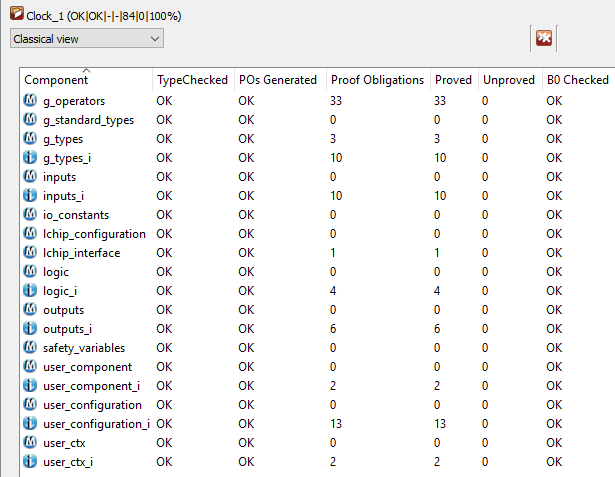
\includegraphics[scale=0.5]{Pictures/chaptProjects/clock1-project-status.png}
\caption{Clock\_1 project status}
\label{projects:Clock_1-project-status}
\end{figure}

The project is ready to be compiled. Be sure that your SK0 board is connected with the USB connector to your host. Right-click on the project name in the left pane and select "CSSP Runner". 
A new window appears, showing a carousel of all the steps of the compilation. Click on the green triangle on the top left. All steps are cleared until the last one where you are asked to reset the SK0 board. Use a pen to push on the reset button and release it. The board starts to blink as it enters bootload mode. After around 30s, the last step is cleared (green check) and you are again invited to reset the SK0 board. Push the reset button and release it. After 2 seconds, the board starts to execute your program.

\section{Testing}

To test your program, you just need to check that, when running, the behaviour is as expected: $0\_1$ beating every second and $0\_2$  is the opposite state of $0\_2$.

\begin{exercise}
Create a program which implements the following equations:
\begin{center}
O$_1$ = not(O$_1$) every second (synchronous)\\
O$_2$ = not(O$_2$) every 2.5 seconds (synchronous)  
\end{center}
First create a new project and populate it with models similar to Clock\_1. Add another constant delta\_t1 valued with 2500. Then modify the body of the operation user\_logic in the component \textit{logic\_i} to implement two clocks over the outputs $0\_1$ and $0\_2$ .
\end{exercise}

%---------------------------------------------------------------------
%	Chapter Clock + combinatorial
%---------------------------------------------------------------------
%\chapterimage{back2.jpg} % Chapter heading image
%\chapter{Clock + combinatorial}

%---------------------------------------------------------------------
%	Chapter Filter
%---------------------------------------------------------------------
%\chapterimage{back2.jpg} % Chapter heading image
%\chapter{Filter}

%=======================================================================
%	PART III: ANNEXES
%=======================================================================

\part{Annexes}
%---------------------------------------------------------------------
%	Chapter Hardware interface
%---------------------------------------------------------------------
\chapterimage{back2.jpg} % Chapter heading image
\chapter{Hardware interface}

The SK$_0$ board is a 10cm x 10 cm x 2 cm board with a weight of 130g. It offers several hardware interfaces to interact with that are listed and explained below.

\begin{figure}[h]
\centering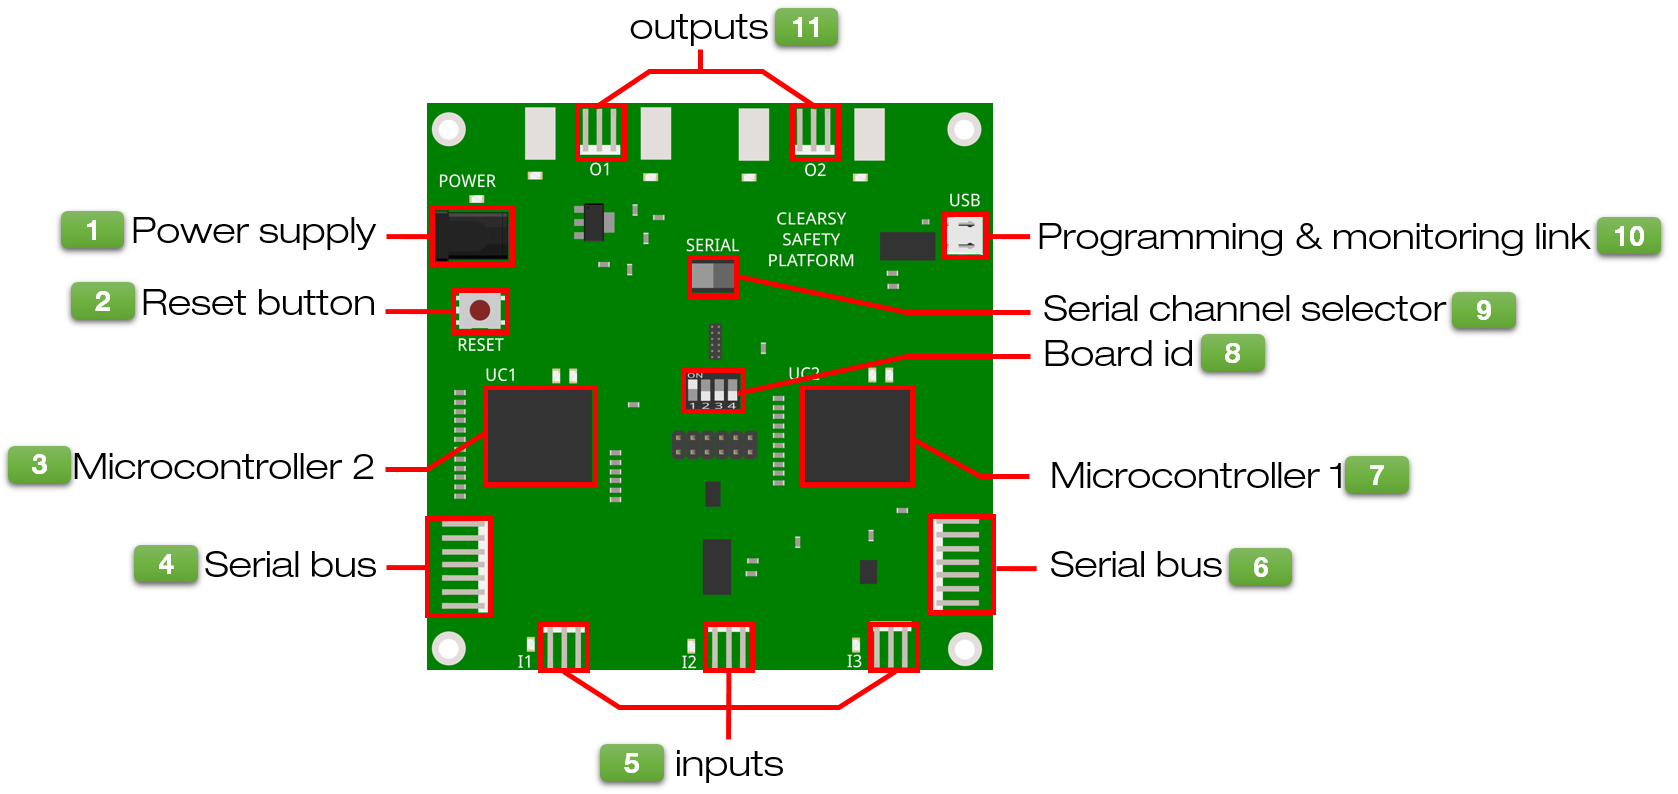
\includegraphics[scale=0.28]{Pictures/chapterAnnexes/SK0-description.png}
\caption{CLEARSY Safety Platform Starter Kit 0}
\label{annexes:SK0-HW-interface}
\end{figure}

\section{Power supply}

It requires +5V DC 500mA. This interface is privileged over USB port, as USB port implementation varies from one computer/equipment to another. We have encountered situations where not enough power was provided to the board, leading to erratic behaviour.

\section{Reset button}

The reset button resets the two microcontrollers at the same time. During the first two seconds after reset, if the bootloader receives a message from the USB port, it will enter bootload mode. If not, the program is copied from flash to RAM and starts its execution on both micro-controllers.

\section{Microcontrollers 1 \& 2}

These are the two PIC32 micro-controllers \footnote{PIC32MX795F512L with 512KB Flash and 128 KB RAM, delivering 105 DMIPS at 80MHz.} installed on the board. They both deliver around 100 DMIPS. As the function defined in \textit{user\_logic} is executed twice in sequence (binary$_1$ than binary$_2$), the SK$_0$ delivers around 50 DMIPS (not counting the execution time of the sequencer and the safety library).

\section{Serial bus}

The serial bus is used to connect several SK$_0$ together (see \S\ref{annexes:SK0-HW-serial-bus} for more information). If only one board is used, this bus is not functional and the board ID has to be 0x0000b.

\section{Inputs}

There are 3 inputs on the board named I$_1$, I$_2$, and I$_3$. \\
\begin{figure}[h]
\centering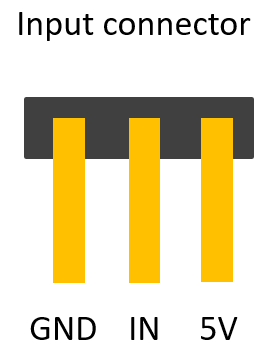
\includegraphics[scale=0.28]{Pictures/chapterAnnexes/sk0-input.png}
\caption{SK$_0$ input connector}
\label{annexes:SK0-input}
\end{figure}
One input (see figure \ref{annexes:SK0-input}) is made of 3 pins:
\begin{itemize}
    \item The ground (GND) is common to all inputs and outputs. In case the board is connected to another device (an Arduino for example), one of these GND pins has to be connected to the other device GND.
    \item The input pin (IN) on which is measured the input voltage.
    \item The +5V pin provides +5V. It has to be used when the input is a switch and not a power line. The switch has to be connected to both pins IN and +5V. This way, when the switch is closed, the current can flow from +5V to IN. 
\end{itemize}

\section{Board ID}
The board ID is made of four bits b$_0$ b$_1$ b$_2$ b$_3$ (see figure \ref{annexes:SK0-boardid}), in order to discriminate the boards when connected together through the serial bus.
\begin{figure}[h]
\centering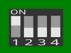
\includegraphics[scale=0.668]{Pictures/chapterAnnexes/boardid.png}
\caption{The board ID set to 0x0001b.}
\label{annexes:SK0-boardid}
\end{figure}
There are some constraints when setting board IDs:
\begin{itemize}
    \item If the board is used alone, its board ID should be 0x0000b (master board).
    \item If the board is connected to other SK$_0$ board(s) through the serial bus, all board IDs have to be different and one board should have the board ID 0x0000b.
\end{itemize}
If no board ID 0x0000b is present, the board(s) will not upload any new software, as the master board is supposed to initiate the upload process. From the user point of view, everything is working properly (from compilation to upload complete) but the program is not flashed in memory and the board is not updated. So always check for the board ID 0x0000b on your system. \\
Modifying the board ID during the execution of the program leads to SK$_0$ entering the panic mode.

\section{Serial channel selector}
This selector is used to select either micro-controller 1 or micro-controller 2 when monitoring the execution of the program. Changing the position of the selector requires reseting the board to be effective.
\begin{figure}[h]
\centering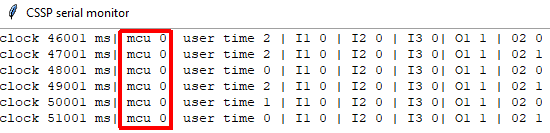
\includegraphics[scale=0.668]{Pictures/chapterAnnexes/traces-channel-selector.png}
\caption{With the CSSP serial monitor, traces indicate that the micro-controller 1 (mcu 0) is being tracked.}
\label{annexes:SK0-channel-selector}
\end{figure}

\section{Programming \& monitoring link}
This is a micro-USB interface for programming (flashing) the board and for monitoring its execution. It could also be used to power the board, but depending on the configuration (PC USB port, USB cable, etc.) behaviour could be unpredictable.

\section{Outputs}
There are 2 outputs on the board named O$_1$ and O$_2$. \\
\begin{figure}[h]
\centering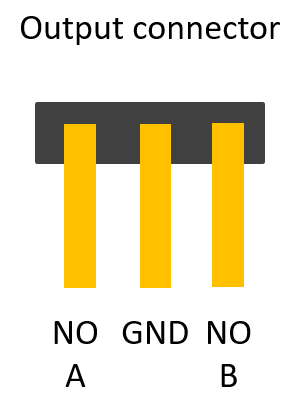
\includegraphics[scale=0.28]{Pictures/chapterAnnexes/sk0-output.png}
\caption{SK$_0$ output connector}
\label{annexes:SK0-output}
\end{figure}\\
One output (see figure \ref{annexes:SK0-output}) is made of 3 pins:
\begin{itemize}
    \item The ground (GND) is common to all inputs and outputs. In case the board is connected to another device (an Arduino for example), one of these GND pins has to be connected to the other device GND.
    \item The "Normally Open" output pin A (NOA).
    \item The "Normally Open" output pin B (NOB).
\end{itemize}
An output is a switch, open or closed. When the switch is closed, the current can flow from the pin NOA to NOB (or from NOB to NOA, depending on how the board is connected to the outside world).

The outputs are not powered by the board. It is your responsibility to connect either NOA or NOB to a current source.



%---------------------------------------------------------------------
%	Chapter LEDS on SK0
%---------------------------------------------------------------------
\chapterimage{back2.jpg} % Chapter heading image
\chapter{LEDS on SK$_0$}


The CLEARSY Safety Platform SK$_0$ is equipped with a number of LEDs providing indications of the board status. Their role is to:
\begin{itemize}
    \item ensure fast checking that the board executes normally
    \item help identifying the root cause of unexpected behaviour
\end{itemize}
 They are listed and explained below.

\begin{figure}[h]
\centering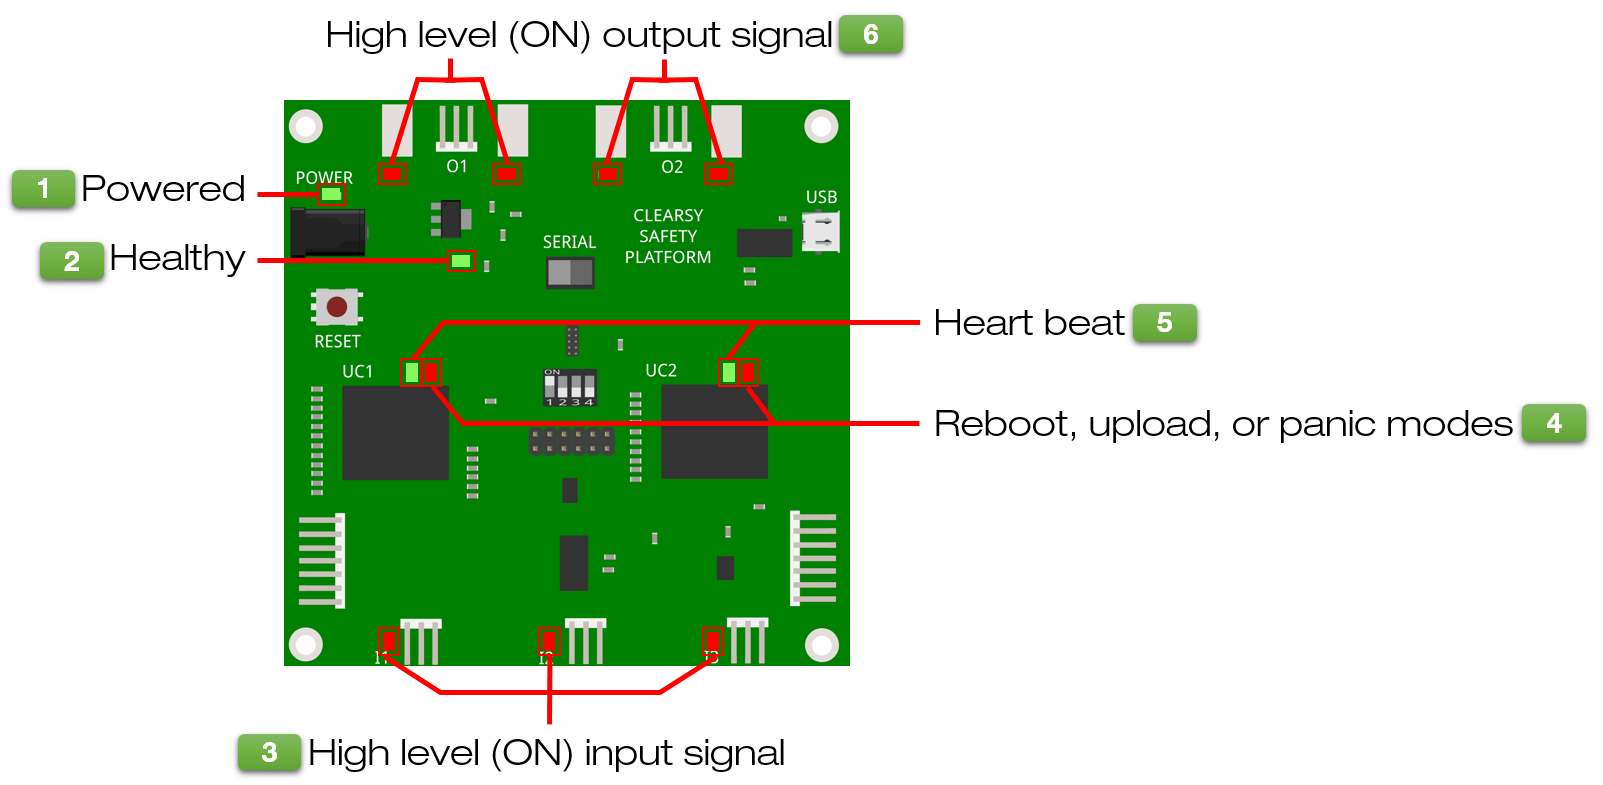
\includegraphics[scale=0.28]{Pictures/chapterAnnexes/SK0-lights.png}
\caption{The LEDs installed on the SK$_0$}
\label{annexes:SK0-HW-light}
\end{figure}

\section{Powered}

This green LED is ON when the board is powered with +5V.
If the LED is not ON, check your power supply.

\section{Healthy}

This green LED is ON when both micro-controllers are powered with +3.3V. This voltage is issued from the main power supply. 

\section{High level input signal}

Each red LED is ON when the electric level of the related input is ON. The input status can also be checked with the CSSP Monitor.
These indications on the electric level of inputs are not guaranteed if the board is only powered by the USB connector.

\section{Reboot, bootload or panic modes}

These two blinking (every second) red LEDs indicate that either the board is rebooting (the program in flash is being copied in memory) or is in bootload mode, erasing the previous program in flash with a new one. Pushing the reset button is required to enter / leave the bootload mode.  \\
The two red LEDs blinking fast indicate a board in panic mode: the outputs are deactivated (circuits are open) and the board enters an infinite loop doing nothing.

\section{Heartbeat}

These two green LEDs blink synchronously every second when the board executes the program in flash memory and is healthy.
\textit{Heartbeat} and \textit{Reboot, bootload or panic modes} LEDs are incompatible: either the former or the latter is ON and blinking.

\section{High level output signal}

Each of the two red LEDs is ON when the electric level of the related output is ON. The output status can also be checked with the CSSP Monitor.
These indications of the electric level of outputs are not guaranteed if the board is only powered by the USB connector.

The outputs are not powered by the board. They are switches. The two red LEDs ON only indicate that the output circuit is closed.

%---------------------------------------------------------------------
%	Chapter CSSP Serial Monitor
%---------------------------------------------------------------------
\chapterimage{back2.jpg} % Chapter heading image
\chapter{CSSP Serial Monitor}

The CSSP Serial Monitor is a feature offered at the project level. It allows to display the log messages emitted by the selected micro-controller on the serial bus. \\
It requires:
\begin{itemize}
    \item one SK$_0$ board to be powered and connected trough its the micro-USB port
    \item the CSSP runner not to be running. The USB communication medium is not shared.
\end{itemize}
To start the CSSP Serial Monitor, select the project, right-click then select "CSSP Monitor". A new window shows up, with 3 buttons (Quit, Pause, and Clear) and a central area containing the text messages emitted by the SK$_0$ board.
\begin{figure}[h]
\centering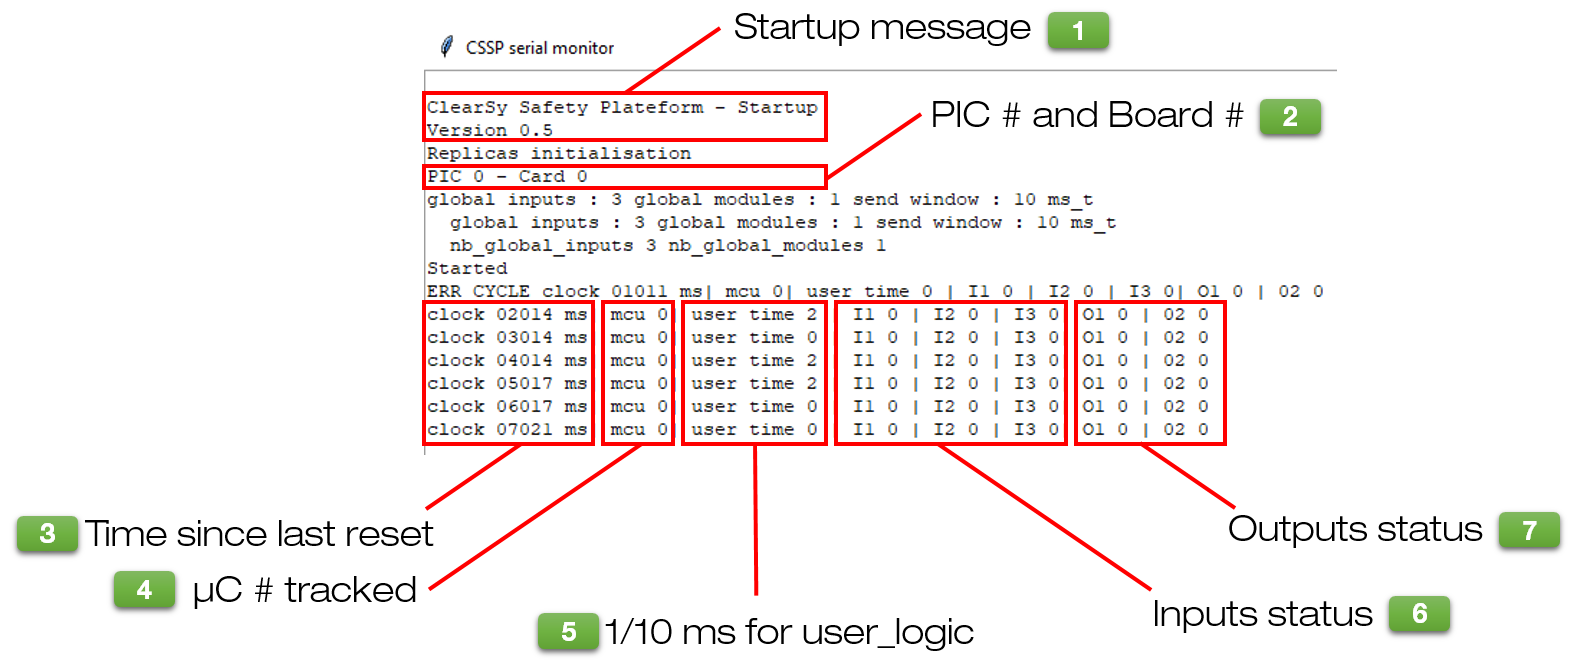
\includegraphics[scale=0.30]{Pictures/chapterAnnexes/traces-serial-monitor.png}
\caption{CSSP Serial Monitor messages}
\label{annexes:SK0-serial-monitor}
\end{figure} \\
As soon as the board is connected and running, the messages are displayed in sequence every second, as shown in figure \ref{annexes:SK0-serial-monitor}. To get all messages including those related to the board configuration, reset the board while the serial monitor is executing. \\
Then you get the following information:
\begin{itemize}
    \item A startup message, providing the version number of the software platform.
    \item The card number and the PIC number being tracked.
    \item The time elapsed since the last reset (in ms).
    \item The micro-controller being tracked (0 or 1).
    \item The time used for the execution of the user\_logic operation during the last cycle (in tenths of ms).
    \item the inputs status (0: OFF, 1: ON).
    \item the outputs status (0: OFF, 1: ON).
\end{itemize}

%---------------------------------------------------------------------
%	Chapter Connecting several boards together
%---------------------------------------------------------------------
\chapterimage{back2.jpg} % Chapter heading image
\chapter{Connecting several boards together}

The board SK$_0$ is aimed at education and hence provides a limited number of inputs and outputs, in order to lower the production price and ease its dissemination. If the systems you are looking for require more inputs and/or outputs, you are advised to consider the board SK$_1$ with 20 inputs and 8 outputs. \\
However an "unsupported feature" allows you to connect several boards SK$_0$ together via their serial bus (see figure \ref{annexes:SK0-HW-serial-bus}). All the boards are connected through a 7-pin connector (each pin is propagated at the same position to the next board). A configuration with \textit{n} boards required  \textit{n-1} connectors. The last board has to be equipped with a terminator with two wires: 
\begin{itemize}
    \item UC1 RX and UC1 TX
    \item UC2 RX and UC2 TX 
\end{itemize}
have to be connected together.
\begin{figure}[h]
\centering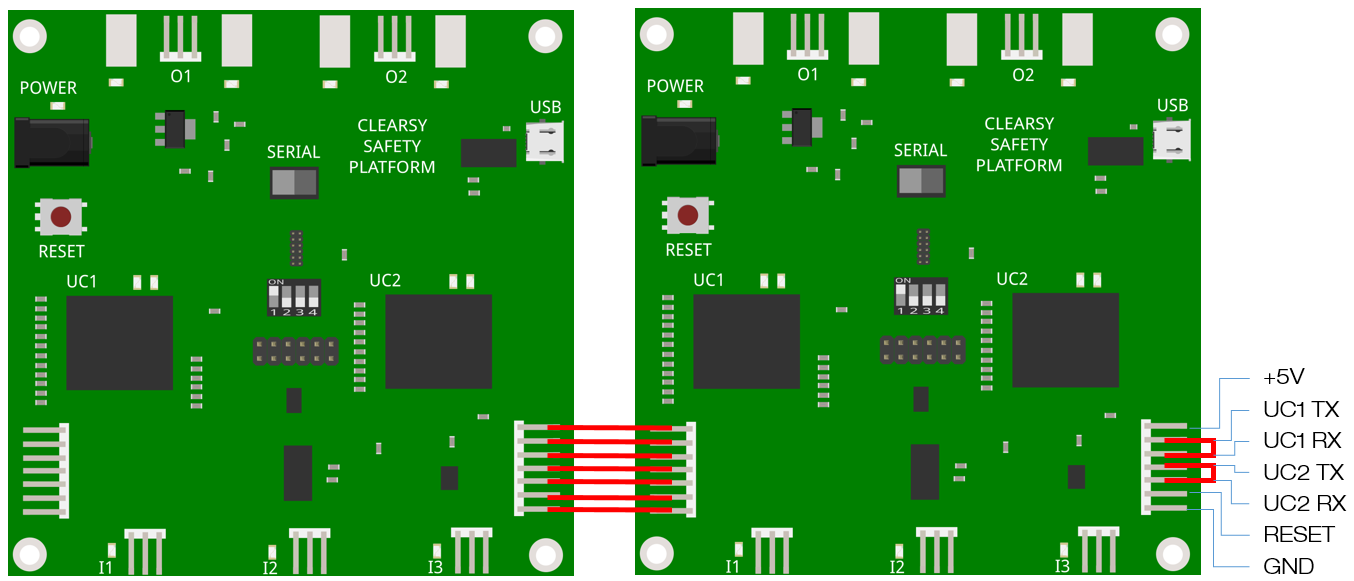
\includegraphics[scale=0.30]{Pictures/chapterAnnexes/SK0-connectinb-boards.png}
\caption{Connecting several SK$_0$ together}
\label{annexes:SK0-HW-serial-bus}
\end{figure} \\
The boards execute exactly the same complete logic, making reference to all inputs and outputs. Inputs acquired by one board are broadcast to other board through the serial bus, at the cost of degraded performance (cycle time is increased with the required data exchange between boards, the higher the number of boards, the longer the cycle time).\\

Board IDs all have to be different. One board has to have the ID 0 (the master board). The boards may be connected in any order. The terminator may be installed on any board.

This feature was developed before SK$_1$ was available. It was used to test the concept but many issues appeared during experiments including jittering distributed clocks. One solution adopted was to have one board initiating the communication (master) and providing a time reference for the other boards. This solution ensures more stability but breaks the safety principles (the master board may be faulty on the time and propagate this error to other boards without means of detection/correction). \\\\
\textbf{\color{ocre}This multi-boards configuration is provided without any support.} 



%---------------------------------------------------------------------
%	Chapter Software interface
%---------------------------------------------------------------------
\chapterimage{back2.jpg} % Chapter heading image
\chapter{Software interface}

The software interface (see figure \ref{annexes:CSSP-SW-interface}) is in two main parts:
\begin{itemize}
    \item \textbf{the interface with the safety library}, containing the definition of all the types (and related constants) that may be used in a CSSP project, as well as specific operators (arithmetic, logic),
    \item \textbf{the model of the function} to program, that has a read-only access to the safety library, the digital inputs status (OFF/ON), the current time since the last reset/power-on, and the ability to modify the digital outputs (OFF/ON)
\end{itemize}
\begin{figure}[h]
\centering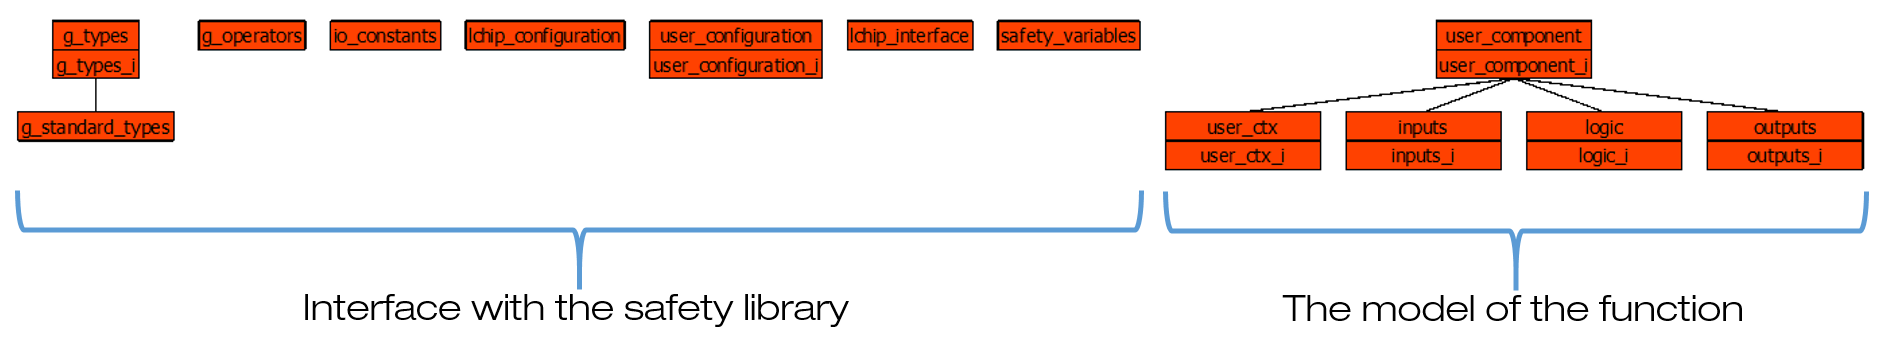
\includegraphics[scale=0.25]{Pictures/chapterAnnexes/sw-interface.png}
\caption{CSSP Software Interface}
\label{annexes:CSSP-SW-interface}
\end{figure}

\section{The interface with the safety library}
\label{annexes:interface-with-safety-library}
%---------------------------------------------------------------------
\subsection{g\_types}

\lstset{frameround=fttt,keywordstyle=\color{ocre}\bfseries}
\lstinputlisting[language=B, frame=trbl, firstline=20,lastline=22,caption={Integer types defined in g\_types}, rulecolor=\color{ocre},label={annexes:g_types_types}]{Models/chapterAnnexes/g_types.mch}

The component g\_types defines the 3 integer types (listing \ref{annexes:g_types_types}) that must be used for implementing arithmetic computations on 8, 16 and 32 bits. No other integer type is available.\\
Components have to define a read-only access (clause SEES - listing \ref{annexes:g_types_sees}) to the component g\_types in order to be able to use any of these 3 types.
\lstset{frameround=fttt,keywordstyle=\color{ocre}\bfseries}
\lstinputlisting[language=B, frame=trbl, firstline=7,lastline=8,caption={Clause SEES to insert in the referring component}, rulecolor=\color{ocre},label={annexes:g_types_sees}]{Models/chapterAnnexes/user_component_i.imp}

%---------------------------------------------------------------------
\subsection{g\_operators}

6 bit-wise operators are defined (listing \ref{annexes:g_op_logic}) for each supported type: uint8\_t, uint16\_t and uint32\_t. These operators are shift-left (\textbf{sll}), shift-right (\textbf{srl}), negation (\textbf{not}), conjunction (\textbf{and}), disjunction (\textbf{or}) and exclusive disjunction (\textbf{xor}). They are defined as constant total functions: 
\begin{itemize}
    \item \textbf{sll} and \textbf{srl} have two parameters: the unsigned integer value to shift, the number of shifts to perform.
    \item \textbf{not} has one parameter: the unsigned integer value to negate.
    \item \textbf{and}, \textbf{or} and \textbf{xor} have two parameters: the unsigned integer values on which to perform logic operation.
\end{itemize}

\lstset{frameround=fttt,keywordstyle=\color{ocre}\bfseries}
\lstinputlisting[language=B, frame=trbl, firstline=37,lastline=42,caption={32-bit bit-wise operators defined in g\_operators},label={annexes:g_op_logic}, rulecolor=\color{ocre}]{Models/chapterAnnexes/g_operators.mch} 
3 arithmetic operators are defined (listing \ref{annexes:g_op_arith}) for each supported type: uint8\_t, uint16\_t and uint32\_t. These operators are addition (\textbf{add}), subtraction (\textbf{sub}), and multiplication (\textbf{mul}). \\
They are defined as constant total functions with two parameters: the unsigned integer values on which to perform arithmetic operation. 
\lstset{frameround=fttt,keywordstyle=\color{ocre}\bfseries}
\lstinputlisting[language=B, frame=trbl, firstline=56,lastline=58,caption={32-bit arithmetic operators defined in g\_operators},label={annexes:g_op_arith}, rulecolor=\color{ocre}]{Models/chapterAnnexes/g_operators.mch}
These operators have been defined to ease the overflow proof\footnote{With B, the result of an addition has to remain in its type. For example, the substitution val := 255+255 cannot be proved if val is defined as uint8\_t as the result (512) exceeds the upper bound of the type. Usually this is solved by adding constraints on operands. }. With the CSSP, these operators are defined as a modulo (upper bound +1) of the result of the operation. For example \\
\begin{center}
add\_uint32(x1, x2) = (x1+x2) mod (MAX\_UINT32+1)
\end{center} where MAX\_UINT32 is the upper bound of the type uint32\_t. This way, the result always remains in the type of the function (8, 16 or 32 bits),the proof is thereby eased and made more automatic.\\


These logic and arithmetic constants have been implemented in the safety library. So they may be used directly in your implementation.

%---------------------------------------------------------------------
\subsection{io\_constants}

This component defines two types (listing \ref{annexes:io_constants}):
\begin{itemize}
    \item TIME, defined over 32-bit integers, used to measure time (expressed in ms) with the operation get\_ms\_tick().
    \item IO\_STATE, defined over 8-bit integers, contains the two valid states of the inputs and outputs: IO\_OFF and IO\_ON. The two values are chosen such that it is very unlikely that a memory perturbation produces the other valid value\footnote{Setting an output with a value different from IO\_OFF or IO\_ON leads the board to enter panic mode.}.
\end{itemize}

\lstset{frameround=fttt,keywordstyle=\color{ocre}\bfseries}
\lstinputlisting[language=B, frame=trbl, firstline=7,lastline=15,caption={Constants defined in io\_constants},label={annexes:io_constants}, rulecolor=\color{ocre}]{Models/chapterAnnexes/io_constants.mch}

%---------------------------------------------------------------------
\subsection{lchip\_configuration}

This component defines three constants (listing \ref{annexes:lchip_configuration}) representing the maximum number of modules, inputs and outputs. This component is mainly aimed at easing the generation of source code and is of little interest for the developer. 
\lstset{frameround=fttt,keywordstyle=\color{ocre}\bfseries}
\lstinputlisting[language=B, frame=trbl, firstline=12,lastline=14,caption={Constants defined in lchip\_configuration},label={annexes:lchip_configuration}, rulecolor=\color{ocre}]{Models/chapterAnnexes/lchip_configuration.mch}

%---------------------------------------------------------------------
\subsection{lchip\_interface}

This component defines several functions:
\begin{itemize}
    \item get\_ms\_tick, which returns the number of milliseconds elapsed since the last rest/power-on (listing \ref{annexes:get_ms_tick}),
    \item read\_global\_input, used to read the status of the digital inputs (used by the component inputs),
    \item write\_global\_output, used to modify the status of the digital outputs (used by the component outputs).
\end{itemize}
\lstset{frameround=fttt,keywordstyle=\color{ocre}\bfseries}
\lstinputlisting[language=B, frame=trbl, firstline=38,lastline=43,caption={Constants defined in lchip\_interface},label={annexes:get_ms_tick}, rulecolor=\color{ocre}]{Models/chapterAnnexes/lchip_interface.mch}

%---------------------------------------------------------------------
\subsection{user\_configuration}

This component defines several constants (listing \ref{annexes:user_configuration}) representing the number of modules, inputs, outputs, and their configuration (IDs). This component is mainly aimed at easing the generation of source code and is of little interest for the developer. 

\lstset{frameround=fttt,keywordstyle=\color{ocre}\bfseries}
\lstinputlisting[language=B, frame=trbl, firstline=8,lastline=21,caption={Constants defined in user\_configuration},label={annexes:user_configuration}, rulecolor=\color{ocre}]{Models/chapterAnnexes/user_configuration.mch}

\section{The model of the function}

The model of the function to program contains 5 components; only two of these may be modified: 
\begin{itemize}
    \item user\_ctx (and its implementation user\_ctx\_i), which contains only constants,
    \item logic (and its implementation logic\_i), which contains only variables and operations.
\end{itemize}

%---------------------------------------------------------------------
\subsection{user\_component}

This component contains the top-level function, user\_app (listing \ref{annexes:user_app}), in charge of reading inputs (operation read\_inputs), performing computation (operation user\_logic) and modifying outputs (operation write\_outputs). \textbf{\color{ocre}This component should not be modified.} 
\lstset{frameround=fttt,keywordstyle=\color{ocre}\bfseries}
\lstinputlisting[language=B, frame=trbl, firstline=23,lastline=29,caption={The top-level operation user\_app},label={annexes:user_app}, rulecolor=\color{ocre}]{Models/chapterAnnexes/user_component_i.imp}

%---------------------------------------------------------------------
\subsection{user\_ctx}

This component contains the constants defined for the function to program. \\

The specification component, user\_ctx (listing \ref{annexes:ctx}), has to declare the constants (clause CONCRETE\_CONSTANTS) and their properties (clause PROPERTIES).

\lstset{frameround=fttt,keywordstyle=\color{ocre}\bfseries}
\lstinputlisting[language=B, frame=trbl, firstline=5,lastline=8,caption={The DELTA\_T constant from the project Clock},label={annexes:ctx}, rulecolor=\color{ocre}]{Models/chapterAnnexes/user_ctx.mch}

The implementation component, user\_ctx\_i (listing \ref{annexes:ctx_i}), has to provide values (clause VALUES) to the constants defined in the component user\_ctx.

\lstset{frameround=fttt,keywordstyle=\color{ocre}\bfseries}
\lstinputlisting[language=B, frame=trbl, firstline=9,lastline=10,caption={Value for the DELTA\_T constant from the project Clock},label={annexes:ctx_i}, rulecolor=\color{ocre}]{Models/chapterAnnexes/user_ctx_i.imp}

%---------------------------------------------------------------------
\subsection{inputs}

\textbf{\color{ocre}This component should not be modified.} \\
It contains:
\begin{itemize}
    \item the variables containing the status of the digital inputs (naming defined by the developer during the creation of the project). They are all defined as 8-bit integers with values in \{IO\_OFF, IO\_ON\}. These variables cannot be modified by other components, only updated when calling the operation read\_inputs.
\end{itemize}
\lstset{frameround=fttt,keywordstyle=\color{ocre}\bfseries}
\lstinputlisting[language=B, frame=trbl, firstline=19,lastline=21,caption={The declaration of the input variables},label=examples:combinatorial-spec, rulecolor=\color{ocre}]{Models/chapterAnnexes/inputs_i.imp} 

\begin{itemize}    
    \item the operations get\_board\_ (the ending depends on the names of the variables) return the status of each digital input, as read by the operation read\_inputs. These operations are called by the operation user\_logic (component logic\_i).
\end{itemize}
\lstset{frameround=fttt,keywordstyle=\color{ocre}\bfseries}
\lstinputlisting[language=B, frame=trbl, firstline=34,lastline=47,caption={The operations get\_board\_},label=examples:combinatorial-spec, rulecolor=\color{ocre}]{Models/chapterAnnexes/inputs_i.imp} 
\begin{itemize}
    \item the operation read\_inputs, modifying the input status variables with the latest physical status read by the board (this operation is called by the top-level operation user\_app).
\end{itemize}
\lstset{frameround=fttt,keywordstyle=\color{ocre}\bfseries}
\lstinputlisting[language=B, frame=trbl, firstline=27,lastline=32,caption={Constants defined in g\_operators},label=examples:combinatorial-spec, rulecolor=\color{ocre}]{Models/chapterAnnexes/inputs_i.imp}

%---------------------------------------------------------------------
\subsection{logic}

This component has to be modified by the developer:
\begin{itemize}
    \item modify the specification of the operation user\_logic (clause OPERATIONS) in the specification model logic.mch (listing \ref{annexes:user_logic_spec}).
\end{itemize}
\lstset{frameround=fttt,keywordstyle=\color{ocre}\bfseries}
\lstinputlisting[language=B, frame=trbl, firstline=9,lastline=19,caption={Variables and operation user\_logic specified in logic.mch},label={annexes:user_logic_spec}, rulecolor=\color{ocre}]{Models/chapterAnnexes/logic.mch}
\begin{itemize}
    \item if required declare additional variables in the implementation model logic\_i.imp (clause CONCRETE\_VARIABLES), then add a type (clause INVARIANT) and an initialisation (clause INITIALISATION) for each of these variables.
    \item modify the implementation of the operation user\_logic (clause OPERATIONS) in the implementation model logic\_i.imp (listing \ref{annexes:user_logic_impl}).    
\end{itemize}
\lstset{frameround=fttt,keywordstyle=\color{ocre}\bfseries}
\lstinputlisting[language=B, frame=trbl, firstline=14,lastline=24,caption={Variables and operation user\_logic implemented in logic\_i.imp},label={annexes:user_logic_impl}, rulecolor=\color{ocre}]{Models/chapterAnnexes/logic_i.imp}
This component also contains operations (listing \ref{annexes:logic_i_get}) to get access to the output status variables, named get\_board\_*, that are generated automatically from the board configuration (naming). \\
\textbf{\color{ocre}The operations get\_board\_ should not be modified.}
\lstset{frameround=fttt,keywordstyle=\color{ocre}\bfseries}
\lstinputlisting[language=B, frame=trbl, firstline=26,lastline=34,caption={Constants defined in g\_operators},label={annexes:logic_i_get}, rulecolor=\color{ocre}]{Models/chapterAnnexes/logic_i.imp}



%---------------------------------------------------------------------
\subsection{outputs}

\textbf{\color{ocre}This component should not be modified.} \\
It contains the operation write\_outputs (listing \ref{annexes:outputs}) that modifies the physical output status with the current output status variables read by the operations get\_board\_ (this operation is called by the top-level operation user\_app).


\lstset{frameround=fttt,keywordstyle=\color{ocre}\bfseries}
\lstinputlisting[language=B, frame=trbl, firstline=13,lastline=24,caption={The write\_outputs operation defined in outputs},label={annexes:outputs}, rulecolor=\color{ocre}]{Models/chapterAnnexes/outputs_i.imp}

%---------------------------------------------------------------------
%	Chapter Stimulating the CSSP
%---------------------------------------------------------------------
%\chapterimage{back2.jpg} % Chapter heading image
%\chapter{Stimulating the CSSP}
% TO DO: to add in the next release

%---------------------------------------------------------------------
%	Chapter Troubleshooting
%---------------------------------------------------------------------
\chapterimage{back2.jpg} % Chapter heading image
\chapter{Troubleshooting}

The CLEARSY Safety Platform combines several technologies which are constrained to fit the safety requirements. Most errors are linked to these restrictions (not all the B0 language is supported in implementation; additional information is required).\\
Some common sources of error:
\begin{itemize}
    \item Using in implementation non-supported operators: +, -, and *. These operators are likely to generate overflow. The integer division / does not generate overflow and as such can be used.
    \item Using in implementation non-supported types: INT, NAT, and STRING.
    \item Writing a 32-bit unsigned int into a 16-bit or 8-bit.
    \item Writing a 16-bit unsigned int into a 8-bit.
    \item Allocating too much memory: table 49k of uint8\_t == 100\% memory
    \item Too many computations preventing inter-MCU verifications (browsing 29k cells of a table)
    \item Panic mode is obtained when there is a memory problem, the program transfer from host to SK0 was interrupted (CRC error) or when the board is unable to perform MCU verification on time.
\end{itemize}
Most error messages linked to models appear in the model editor (typecheck, compliancy with implementable language) or in the bottom pane (Errors \& warnings) of the main window. 
Some more insidious errors located in the double compilation chain (DCC) may appear:
\begin{itemize}
    \item in the runner window 
    \item or in the dcc\_build/log directory. For each compilation, one log file is generated (project name, date, time). For this file, search for error messages at the end of the file like "bxml error".
\end{itemize}



%---------------------------------------------------------------------
%	GLOSSARY
%---------------------------------------------------------------------
\chapter*{Glossary}


\begin{vocabulary}[Atelier B]
CASE tool implementing the B method
\end{vocabulary}

\begin{vocabulary}[CSSP]
Abbreviation for CLEARSY Safety Platform
\end{vocabulary}

\begin{vocabulary}[Proof Obligation]
Mathematical predicate that needs to be demonstrated to prove a model. Non trivial models are made of hundreds/thousands of proof obligations.
\end{vocabulary}

\begin{vocabulary}[SIL\{3/4\}]
Safety Integrity Level. Defines the level of safety (the higher the safer) of a system - ranging between 0 and 4. Also refers to the level of danger of a system: a SIL4 system is considered to be able to kill people in case of catastrophic failure while a SIL0 system has no chance to harm someone.
\end{vocabulary}

\begin{vocabulary}[2oo2]
Put for "2 out of 2". Means that a computation performed twice with different means is successful only if the two computations are identical. 2oo3 allows to have a system operated in the case that one of its three computers is behaving differently from the two others.
\end{vocabulary}


%---------------------------------------------------------------------
%	SYMBOLS TABLE
%---------------------------------------------------------------------

\chapter*{Symbols Table}
%\addcontentsline{toc}{chapter}{\textcolor{ocre}{Symbols Table}}

This appendix contains the description of reserved keywords and of the operators of B language, sorted by ascending ASCII order.\\
For each reserved keyword or operator, this chapter provides:
\begin{itemize}
    \item its \textbf{ASCII notation}, 
    \item its \textbf{mathematical notation}, if it differs from its ASCII notation.
    \item its \textbf{priority level}. The priority level corresponds to the priority level during the syntactic analysis. The higher the priority level of an operator, the more it attracts operands. For example, if the operators op40 and op250 are respectively of 40 and 250 priority, then the expression x op40 y op250 z is analysed as x op40 (y op250 z)
    \item its \textbf{associative properties} (L for associative to the left or R for associative to the right). If two binary operators named op have the same priority, then: x op y op z will be analysed as (x op y) op z if op is associative to the left; and as x op (y op z) if op is associative to the right.
    \item its \textbf{description}.
\end{itemize}
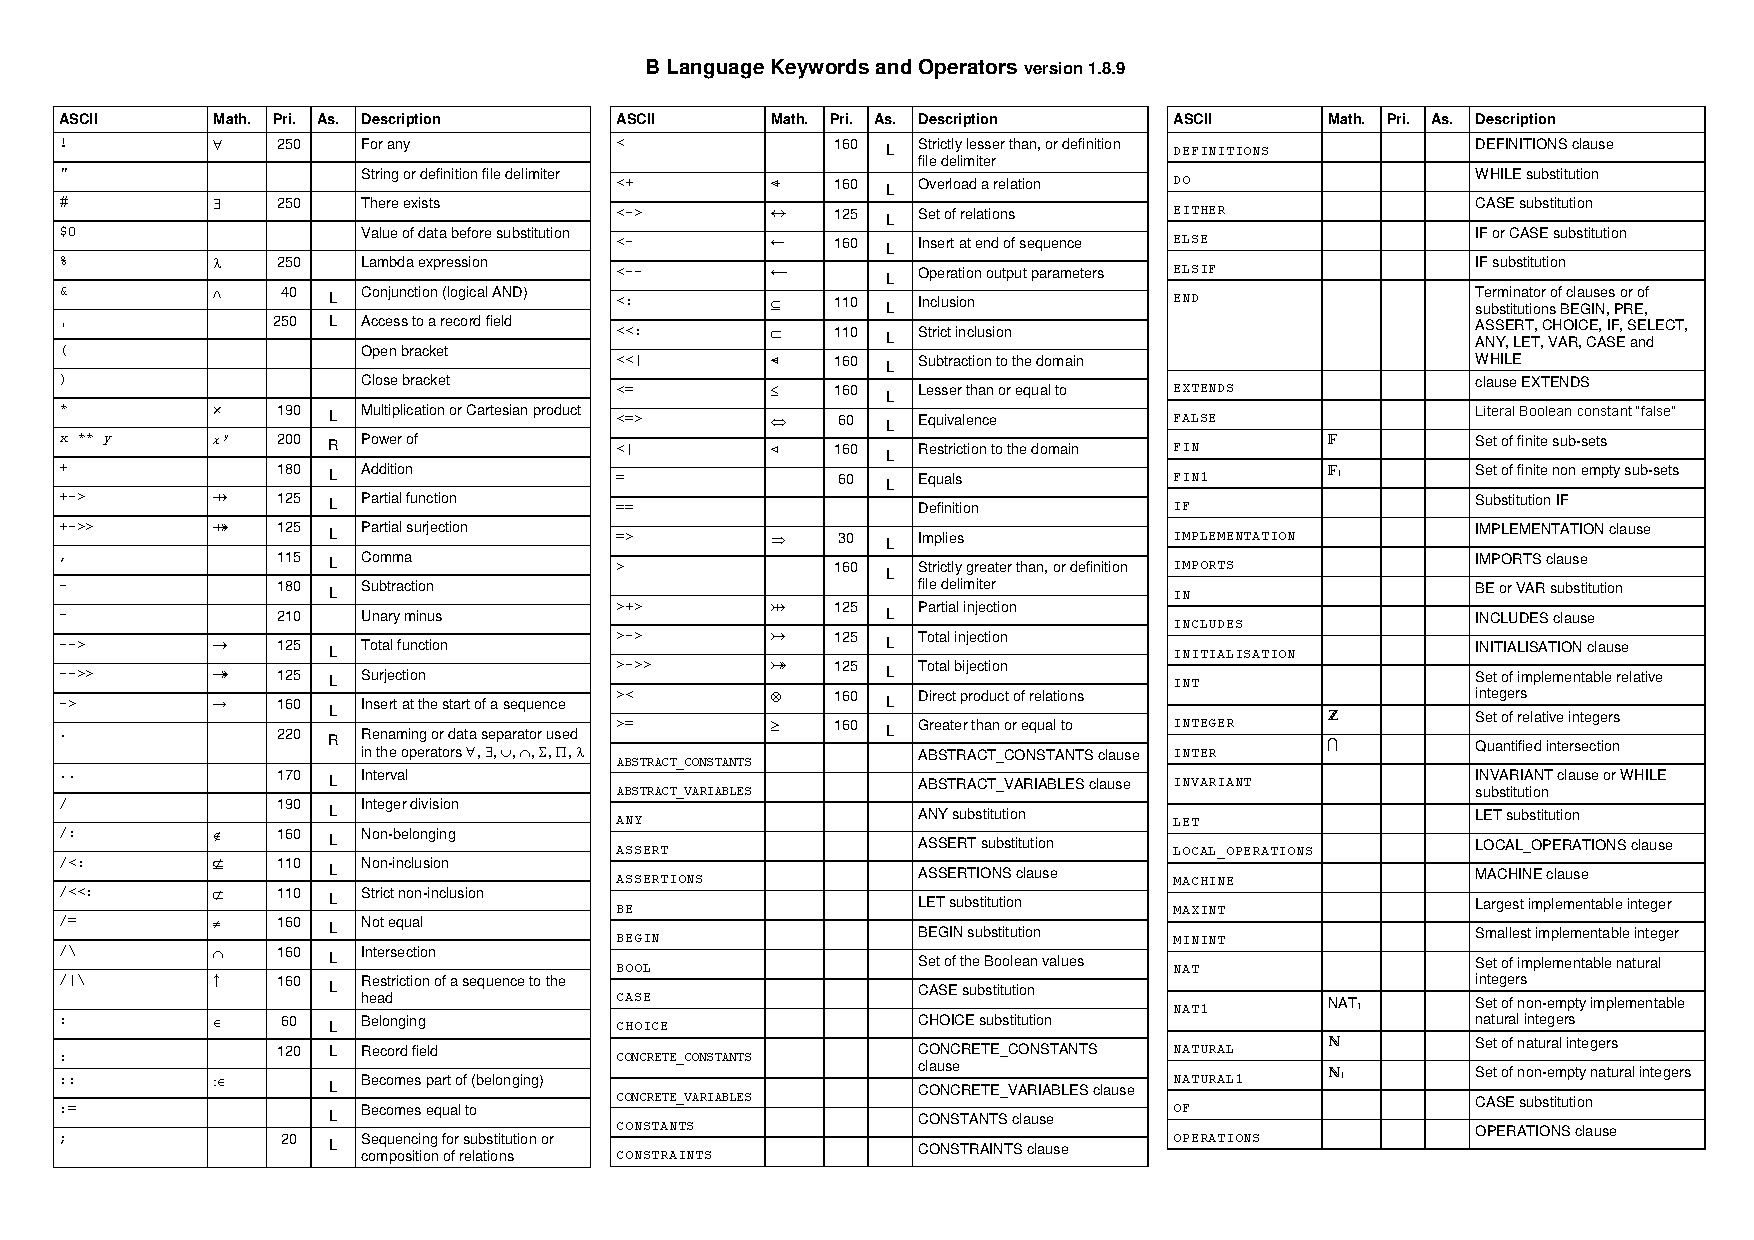
\includepdf[pages={1},landscape=true]{symboles-uk}
\includepdf[pages={2},landscape=true]{symboles-uk}

%----------------------------------------------------------------------------------------
%	BIBLIOGRAPHY
%----------------------------------------------------------------------------------------

\chapter*{Bibliography}
%\addcontentsline{toc}{chapter}{\textcolor{ocre}{Bibliography}}
\section*{Books}
%\addcontentsline{toc}{section}{Books}
\printbibliography[heading=bibempty,type=book]
\section*{Articles}
%\addcontentsline{toc}{section}{Articles}
\printbibliography[heading=bibempty,type=article]
%\printbibliography[heading=bibempty,type=article]


%----------------------------------------------------------------------------------------
%	INDEX
%----------------------------------------------------------------------------------------

\cleardoublepage
\phantomsection
\setlength{\columnsep}{0.75cm}
%\addcontentsline{toc}{chapter}{\textcolor{ocre}{Index}}
\printindex

%----------------------------------------------------------------------------------------

\end{document}